% ============================================================
% 2026年北京理工大学数学建模竞赛第三轮
% 论文标题：基于弹性悬链线与多目标动态优化的溜索系统安全与体验设计模型
% ============================================================
\documentclass[12pt,a4paper]{ctexart}

% ---------- 页面设置 ----------
\usepackage[top=2.5cm, bottom=2.5cm, left=2.5cm, right=2.5cm]{geometry}
\usepackage{fancyhdr}
\usepackage{graphicx}
\usepackage{float}
\usepackage{amsmath,amssymb}
\usepackage{booktabs}
\usepackage{array}
\usepackage{multirow}
\usepackage{caption}
\usepackage{subcaption}
\usepackage{tikz}
\usepackage{pgfplots}
\pgfplotsset{compat=1.18}
\usepackage{algorithm}
\usepackage{algorithmicx}
\usepackage{algpseudocode}
\usepackage[colorlinks=true,linkcolor=black,citecolor=black,urlcolor=black]{hyperref}
\usepackage{enumitem}
\usepackage{xcolor}
\usepackage{listings}
\usepackage{setspace}

% ---- Python代码高亮样式 ----
\lstdefinestyle{pythonstyle}{
  language=Python,
  basicstyle=\small\ttfamily,
  keywordstyle=\color{blue!70!black}\bfseries,
  commentstyle=\color{green!50!black},
  stringstyle=\color{orange!80!black},
  numberstyle=\tiny\color{gray},
  numbers=left,
  numberblanklines=false,
  stepnumber=1,
  numbersep=6pt,
  backgroundcolor=\color{gray!5},
  frame=single,
  framerule=0.6pt,
  rulecolor=\color{gray!40},
  breaklines=true,
  breakatwhitespace=false,
  tabsize=4,
  showstringspaces=false,
  captionpos=b,
  xleftmargin=2em,
  framexleftmargin=1.5em,
  aboveskip=8pt,
  belowskip=8pt,
  columns=flexible,
  upquote=true,
}
\lstset{style=pythonstyle}

% ---------- 页眉页脚 ----------
\fancypagestyle{plain}{%
  \fancyhf{}
  \fancyfoot[C]{\thepage}
  \renewcommand{\headrulewidth}{0pt}
}
\pagestyle{plain}

% 正文页码从摘要后开始
% 承诺书页不编号，摘要页开始编号

% ---------- 正文行距 ----------
\setstretch{1.25}

\begin{document}

% ============================================================
% 第1页：参赛承诺书（不编页码）
% ============================================================
\thispagestyle{empty}
\pagenumbering{gobble}

\begin{center}
  {\LARGE\bfseries 参赛承诺书}
\end{center}

\vspace{1.5cm}

提交包含此承诺书的pdf文件，表明所有此文件的作者共同承诺：

\vspace{0.8cm}

我们完全清楚，在竞赛开始后参赛队员不能以任何方式，包括电话、电子邮件、``贴吧''、QQ群、微信群等，与队外的任何人（包括指导教师）交流、讨论与赛题有关的问题；无论主动参与讨论还是被动接收讨论信息都是严重违反竞赛纪律的行为。

\vspace{0.8cm}

我们以中国大学生名誉和诚信郑重承诺，严格遵守竞赛章程和参赛规则，以保证竞赛的公正、公平性。如有违反竞赛章程和参赛规则的行为，我们将受到严肃处理。

\vspace{0.8cm}

我们授权北京理工大学数学建模竞赛组织方，可将我们的论文以任何形式进行公开展示（包括进行网上公示，在书籍、期刊和其他媒体进行正式或非正式发表等）。

\vspace{2cm}

\begin{flushright}
  2026年7月
\end{flushright}

\newpage

% ============================================================
% 第2页：摘要专用页
% ============================================================
\thispagestyle{empty}

\begin{center}
  {\LARGE\bfseries 基于弹性悬链线与多目标动态优化的\\[6pt]溜索系统安全与体验设计模型}
\end{center}

\vspace{1cm}

\noindent{\large\bfseries 摘要}

\vspace{0.6cm}

\noindent
针对大跨度低高差溜索（$W=600$\,m, $H/W<0.04$）中低势能余量与多体重兼容的物理矛盾，本文构建了弹性悬链线静力学—非线性动力学—多目标优化三层递进模型，提出``前置测速+单次恒定制动''的半闭环自适应控制策略——在缓冲启动前利用体重与速度测量完成一次反馈修正，进入缓冲段后制动力保持恒定，属于``前置测量反馈+单次恒定执行''策略。

\textbf{问题一}建立弹性悬链线微元平衡方程，引入胡克定律推导无应力原长与受力后几何长度的变形协调关系，以弧长残差构造打靶法迭代求解水平张力。以FEM铰接杆单元非线性规划进行独立交叉校验，线形偏差$<0.03\%$。动力学预演表明松缆工况末端驱动力不足，为紧缆设计提供物理依据。

\textbf{问题二}构建沿弧长切向的非线性动力学ODE系统，采用自适应步长RK4求解。基于Kleiber异速生长法则修正迎风面积（$A(m)\propto m^{2/3}$），修正了定常面积假设对轻体重游客阻力的高估缺陷。对恒定缓冲摩擦力进行网格搜索与可行域分析，揭示了在紧缆工况下单一恒定力无法同时满足30--80\,kg全体重安全的物理死锁。

\textbf{问题三}提出``前置测速+单次恒定制动''策略：在距终点$d_b$处测速，基于能量守恒逆解使游客末速收敛至目标值的恒定制动力$B_{\text{target}}(m,v_{\text{pre}})$，进入缓冲段后力严格保持恒定。采用NSGA-II求解满意度--安全度双目标优化，TOPSIS筛选最终方案。针对参数不确定性的鲁棒性分析表明，分体重运营策略——40--80\,kg采用前置测速恒定制动（安全通过率约92.5\%），30--40\,kg辅以微下倾接站平台——可在全体重范围内实现可靠安全保障。

\vspace{1cm}

\noindent{\large\bfseries 关键词}

\vspace{0.4cm}

\noindent 弹性悬链线；滑行动力学；恒定制动；多目标优化；溜索安全

\newpage

% ============================================================
% 目录页
% ============================================================
\thispagestyle{empty}
\tableofcontents
\newpage

% ============================================================
% 正文开始，页码从1开始
% ============================================================
\pagenumbering{arabic}
\setcounter{page}{1}

% ---------- 正文标题 ----------
\begin{center}
  {\LARGE\bfseries 基于弹性悬链线与多目标动态优化的\\[6pt]溜索系统安全与体验设计模型}
\end{center}

\vspace{0.6cm}

% ============================================================
% 一、问题背景与分析
% ============================================================
\section{问题背景与分析}

\subsection{问题背景}

钢缆溜索是山地、峡谷景区广泛设置的体验项目，由两端固定的主钢缆和滑动吊具组成。游客通过吊具沿钢缆滑行，体验高速穿越的快感。然而，溜索设计面临一个核心矛盾：速度越快，刺激感越强，但终点速度必须控制在3.5\,m/s以内以确保安全着陆。此外，景区面向体重差异显著（30--80\,kg）的多样化游客群体，同一套物理参数必须同时满足所有人的安全要求。

\subsection{问题分析}

深入分析题目可知，溜索系统中存在四个关键的非线性特征：

\begin{enumerate}[label=(\arabic*),leftmargin=2em]
  \item \textbf{钢缆弹性导致形态非线性}：钢缆在自重和集中载荷作用下产生弹性伸长，形变后的弧长与张力分布相互耦合，传统不可伸长悬链线模型已不适用；
  \item \textbf{空气阻力导致速度非线性}：滑行速度范围内空气阻力与速度平方成正比，使得速度变化呈非线性衰减特征；
  \item \textbf{滚动摩擦力随位置变化}：切线角变化导致法向载荷分量$mg\cos\theta(x)$随位置改变，形成位置依赖的摩擦力分布；
  \item \textbf{控制闭环引入决策非线性}：前置测速策略将制动力设计为质量$m$和前置速度$v_{\text{pre}}$的非线性函数$B_{\text{target}}=f(m,v_{\text{pre}})$（式\ref{eq:btarget}），由此构成"物理状态$\to$测速$\to$能量逆解$\to$制动输出"的决策闭环。该闭环使得目标函数与决策变量之间的关系不再具有闭合解析梯度，传统的线性规划或梯度下降方法失效，必须采用启发式多目标进化算法（NSGA-II）进行全局寻优。
\end{enumerate}

上述四个非线性特征——几何非线性、气动非线性、摩擦非线性和控制非线性——决定了不能采用能量守恒等准静态方法粗略估算，必须从静力学平衡方程出发求解弹性悬链线形态，再基于瞬时受力分析建立动力学微分方程进行数值求解，最终通过进化算法在无梯度条件下完成系统级多目标优化。整体建模思路如图\ref{fig:workflow}所示。

\begin{figure}[H]
  \centering
  \begin{tikzpicture}[node distance=2.5cm, auto,
      block/.style={rectangle, draw, fill=blue!10, text width=6cm, text centered, rounded corners, minimum height=1.2cm},
      arrow/.style={->, thick}]
    \node [block] (P1) {\textbf{问题一：弹性悬链线静力学}\\打靶法求解$H_0$，输出$y(x), \theta(x), T(x)$};
    \node [block, below of=P1] (P2) {\textbf{问题二：非线性动力学}\\RK4求解ODE，网格搜索缓冲可行域};
    \node [block, below of=P2] (P3) {\textbf{问题三：多目标优化}\\NSGA-II + TOPSIS，输出最优参数组合};
    \draw [arrow] (P1) -- (P2);
    \draw [arrow] (P2) -- (P3);
  \end{tikzpicture}
  \caption{整体建模思路流程图}
  \label{fig:workflow}
\end{figure}


% ============================================================
% 二、模型假设与符号说明
% ============================================================
\section{模型假设与符号说明}

\subsection{模型假设}

为建立合理且可求解的数学模型，提出以下假设：

\begin{enumerate}[label=(\arabic*),leftmargin=2em]
  \item \textbf{钢缆材质均匀且各向同性}：假设钢缆材料满足胡克定律，弹性模量$E$为常数，为引入弹性形变提供合法物理依据；
  \item \textbf{钢缆为理想柔索}：仅承受轴向拉力，不承受弯矩和剪力，变形后形态由张力平衡唯一确定；
  \item \textbf{人员与吊具视为质点}：忽略吊具尺寸和人员姿态变化，以单一质量点代表载人状态；
  \item \textbf{吊具与钢缆为线接触}：滑轮与钢缆存在有限接触长度$L_{\text{contact}}$，法向载荷包含重力分量$mg\cos\theta$和钢缆张力通过曲率诱发的附加法向压力$T\kappa L_{\text{contact}}$两项；
  \item \textbf{风载荷视为恒定阻力}：不考虑高频风振和阵风效应，仅以等效恒定阻力叠加处理；
  \item \textbf{迎风面积服从异速生长法则}：人体迎风面积与体重的$2/3$次方成正比，即$A(m) = A_{\text{ref}} \cdot (m/m_{\text{ref}})^{2/3}$，其中$A_{\text{ref}} = 0.4$\,m$^2$为80\,kg成年人坐姿参考面积。该法则源自生物力学异速生长理论（Kleiber法则\cite{kleiber1947}），避免了对轻体重游客阻力的过高估计；
  \item \textbf{不考虑钢缆横向振动}：人员滑行过程中钢缆的横向振动对滑行速度的影响忽略不计。
  \item \textbf{体重由出发前称重获得}：游客出发前由吊具称重传感器或站台电子秤获得体重$m$，与前置测速点$v_{\text{pre}}$共同输入制动力计算模块。在蒙特卡洛鲁棒性分析中，体重测量误差相对较小（$\sim\pm1$\,kg），暂未纳入不确定性建模。
\end{enumerate}

\subsection{符号说明}

\begin{table}[H]
  \centering
  \caption{符号说明表}
  \label{tab:symbols}
  \renewcommand{\arraystretch}{1.1}
  \begin{tabular}{c|c|c|c}
    \toprule
    \textbf{类别} & \textbf{符号} & \textbf{含义} & \textbf{单位} \\
    \midrule
    \multirow{6}{*}{几何参数}
      & $W$   & 两岸固定点水平距离 & m \\
      & $H$   & 两岸固定点高差 & m \\
      & $L$   & 钢缆总长 & m \\
      & $A$   & 钢缆截面积 & m$^2$ \\
      & $x_0$ & 人员水平位置 & m \\
      & $\alpha_{\text{cable}}$ & 钢缆松紧角 & rad \\
    \midrule
    \multirow{5}{*}{物理参数}
      & $R$   & 钢缆线密度 & kg/m \\
      & $E$   & 钢缆弹性模量 & Pa \\
      & $\rho_{\text{steel}}$ & 钢材密度 & kg/m$^3$ \\
      & $m$   & 人员体重 & kg \\
      & $g$   & 重力加速度 & m/s$^2$ \\
    \midrule
    \multirow{5}{*}{力学参数}
      & $T(x)$   & 钢缆$x$处张力 & N \\
      & $H_0$    & 水平张力分量（常数） & N \\
      & $V(x)$   & 垂直张力分量 & N \\
      & $y(x)$   & 钢缆$x$处竖直坐标（以起点为参考零点） & m \\
      & $d(x)$   & 钢缆$x$处垂度（相对两端连线的挠度） & m \\
    \midrule
    \multirow{5}{*}{运动学参数}
      & $v(t)$         & 人员滑行速度 & m/s \\
      & $v^{(m)}_{\max}$ & 体重$m$人员的最大速度 & m/s \\
      & $v^{(m)}_{\text{end}}$ & 体重$m$人员的终点速度 & m/s \\
      & $a(t)$         & 滑行加速度 & m/s$^2$ \\
      & $s(t)$         & 沿钢缆弧长位移 & m \\
    \midrule
    \multirow{6}{*}{阻力参数}
      & $C_d$       & 空气阻力系数 & -- \\
      & $\rho_{\text{air}}$ & 空气密度 & kg/m$^3$ \\
      & $A_{\text{frontal}}$ & 迎风面积 & m$^2$ \\
      & $\mu_{\text{roll}}$ & 滚动摩擦系数 & -- \\
      & $\mu_{\text{cable}}$ & 钢缆--滑轮滑动摩擦系数 & -- \\
      & $L_{\text{contact}}$ & 滑轮--钢缆接触长度 & m \\
    \midrule
    \multirow{4}{*}{优化参数}
      & $d_b$ & 缓冲启动距终点水平距离 & m \\
      & $x_b = W-d_b$ & 缓冲启动水平坐标（起点$x=0$） & m \\
      & $B_{\text{target}}$   & 恒定制动力（能量逆解） & N \\
      & $\Delta L_{\text{elastic}}$ & 钢缆弹性伸长量 & m \\
      & $\mathbf{X}$         & 决策向量 & -- \\
    \bottomrule
  \end{tabular}
\end{table}

关键力学参数来源详见表\ref{tab:param_sources}。

\begin{table}[H]
  \centering
  \caption{关键力学参数取值与来源}
  \label{tab:param_sources}
  \renewcommand{\arraystretch}{1.2}
  \begin{tabular}{c|c|c|c}
    \toprule
    \textbf{参数} & \textbf{取值} & \textbf{来源} & \textbf{参与灵敏度/蒙特卡洛} \\
    \midrule
    $R$ & 1.2\,kg/m & 题目给定 & 否 \\
    $C_d$ & 0.7 & 工程经验取值（钝体绕流），蒙特卡洛扰动检验 & 是 \\
    $A_{\text{ref}}$ & 0.4\,m$^2$ & 人体坐姿投影面积工程估算 & 是（通过异速生长法则） \\
    $\mu_{\text{roll}}$ & 0.005 & 工程经验取值（滚动轴承），蒙特卡洛扰动检验 & 是 \\
    $\mu_{\text{cable}}$ & 0.025 & 工程经验取值（滑轮组） & 否 \\
    $\sigma_b$ & 1770\,MPa & GB/T 20118--2017\cite{GB-T20118} & 否 \\
    $[K]_{\min}$ & 4.0 & GB 12352--2018\cite{GB12352} & 否 \\
    $v_{\text{limit}}$ & 3.5\,m/s & 题目给定 & 否 \\
    $|a|_{\max}$ & 5.0\,m/s$^2$ & 工程经验取值（乘客舒适度） & 否 \\
    $|J|_{\max}$ & 10.0\,m/s$^3$ & 工程经验取值（乘客舒适度） & 否 \\
    \bottomrule
  \end{tabular}
\end{table}
\section{问题一：弹性悬链线与静力学分析模型}

\subsection{模型选取与建立}

传统刚体悬链线模型假设钢缆不可伸长（$E \to \infty$），仅适用于小跨度、低应力场景。对跨度$W = 600$\,m的溜索，钢缆自重导致的弹性伸长量不可忽略。本文建立考虑弹性形变的悬链线模型。

\subsubsection{微元受力平衡}

\begin{figure}[H]
  \centering
  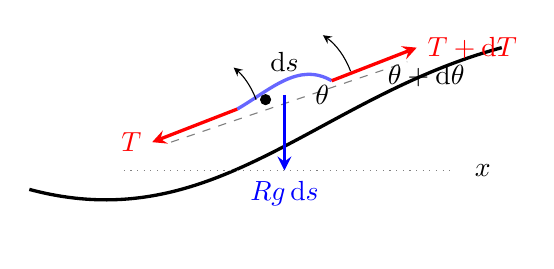
\begin{tikzpicture}[scale=1.2,>=stealth]
    % 钢缆曲线段 (微元ds) — 悬链线下垂形态
    \draw[very thick] (0,0) to[out=-15,in=195] (5,1.5);
    % 微元高亮
    \draw[very thick, blue!60] (2.2,0.85) to[out=30,in=150] (3.2,1.15);
    \filldraw (2.5,0.95) circle (1.5pt);
    % 切线方向
    \draw[dashed, gray] (1.5,0.5) -- (4.0,1.35);
    % 标注微元
    \node at (2.7,1.35) {$\mathrm{d}s$};
    % 左端张力
    \draw[->, red, very thick] (2.2,0.85) -- (1.3,0.5) node[left] {$T$};
    % 右端张力
    \draw[->, red, very thick] (3.2,1.15) -- (4.1,1.5) node[right] {$T+\mathrm{d}T$};
    % 重力
    \draw[->, blue, very thick] (2.7,1.0) -- (2.7,0.2) node[below] {$Rg\,\mathrm{d}s$};
    % 角度标注
    \draw[->] (2.2,0.85) ++(0.2,0.1) arc[start angle=20, end angle=50, radius=0.8];
    \node at (3.1,1.0) {$\theta$};
    \draw[->] (3.2,1.15) ++(0.2,0.1) arc[start angle=20, end angle=55, radius=0.8];
    \node at (4.2,1.2) {$\theta+\mathrm{d}\theta$};
    % 水平参考线
    \draw[dotted, gray] (1.0,0.2) -- (4.5,0.2);
    \node at (4.8,0.2) {$x$};
  \end{tikzpicture}
  \caption{钢缆微元受力分析示意图}
  \label{fig:microelement}
\end{figure}

取钢缆微元$\mathrm{d}s$进行受力分析。设$T$为切向张力，$\theta$为切线与水平方向夹角。受力平衡方程为：

\begin{equation}
  \frac{\mathrm{d}}{\mathrm{d}x}\left(T\cos\theta\right) = 0 \quad\Rightarrow\quad H_0 = T\cos\theta = \text{const}
  \label{eq:h_const}
\end{equation}

\begin{equation}
  \frac{\mathrm{d}}{\mathrm{d}x}\left(T\sin\theta\right) = Rg\frac{\mathrm{d}s}{\mathrm{d}x}
  \label{eq:v_balance}
\end{equation}

由式(\ref{eq:h_const})知水平张力$H_0$为常数。垂直方向积分得：

\begin{equation}
  V(x) = H_0\tan\theta = H_0\frac{\mathrm{d}y}{\mathrm{d}x}
  \label{eq:tan_theta}
\end{equation}

由$\mathrm{d}s = \sqrt{1 + (y')^2}\,\mathrm{d}x$，代入式(\ref{eq:v_balance})得：

\begin{equation}
  H_0\frac{\mathrm{d}^2y}{\mathrm{d}x^2} = Rg\sqrt{1 + \left(\frac{\mathrm{d}y}{\mathrm{d}x}\right)^2}
  \label{eq:catenary_ode}
\end{equation}

式(\ref{eq:catenary_ode})即为经典悬链线微分方程，其解析解为：

\begin{equation}
  y(x) = \frac{H_0}{Rg}\cosh\left(\frac{Rg}{H_0}x + C_1\right) + C_2
  \label{eq:catenary_analytic}
\end{equation}

\subsubsection{弹性变形协调}

引入胡克定律：微元在张力$T$作用下的实际伸长量为原长的$T/(EA)$倍。设受力后悬链线的几何微元弧长为：

\begin{equation}
  \mathrm{d}s_{\text{geo}} = \sqrt{1 + \left(\frac{\mathrm{d}y}{\mathrm{d}x}\right)^2}\,\mathrm{d}x
  \label{eq:ds_geo}
\end{equation}

则无应力原长微元$\mathrm{d}s_0$由受力后几何长度回退弹性伸长量得到：

\begin{equation}
  \mathrm{d}s_0 = \frac{\mathrm{d}s_{\text{geo}}}{1 + \frac{T(x)}{EA}}
  \label{eq:hooke_ds}
\end{equation}

其中截面积$A = R / \rho_{\text{steel}}$，$\rho_{\text{steel}} = 7850$\,kg/m$^3$（钢材密度）。钢缆无应力总长（出厂长度）约束方程为：

\begin{equation}
  \int_{0}^{W} \frac{\sqrt{1 + \left(\frac{\mathrm{d}y}{\mathrm{d}x}\right)^2}}{1 + \frac{T(x)}{EA}}\,\mathrm{d}x = L
  \label{eq:total_length}
\end{equation}

高差约束方程为：

\begin{equation}
  \int_{0}^{W} \frac{\mathrm{d}y}{\mathrm{d}x}\,\mathrm{d}x = y(W) - y(0) = H
  \label{eq:height_diff}
\end{equation}

\subsubsection{载人集中力处理}

当人员位于$x = x_0$时，在该位置处钢缆张力发生突变。垂直方向增加集中力$mg$。设$V_-(x_0)$和$V_+(x_0)$分别为人员左侧和右侧的垂直张力分量：

\begin{equation}
  V_+(x_0) - V_-(x_0) = mg
  \label{eq:concentrated_force}
\end{equation}

载人状态下，将钢缆分为$[0, x_0]$和$[x_0, W]$两段分别求解悬链线方程，在分段点$x_0$处满足力平衡条件(\ref{eq:concentrated_force})和位移连续条件。载人悬链线方程的显式分段表达式为：

\begin{equation}
  y_{\text{loaded}}(x) =
  \begin{cases}
    \displaystyle \frac{H_0}{Rg}\,\cosh\!\left(\frac{Rg}{H_0}x + C_{1L}\right) + C_{2L}, & 0 \leq x \leq x_0 \\[12pt]
    \displaystyle \frac{H_0}{Rg}\,\cosh\!\left(\frac{Rg}{H_0}x + C_{1R}\right) + C_{2R}, & x_0 < x \leq W
  \end{cases}
  \label{eq:loaded_catenary}
\end{equation}

其中$H_0$在分段点两侧保持相等以保证水平张力连续（无水平集中外力）。四个积分常数$C_{1L}, C_{2L}, C_{1R}, C_{2R}$以及$x_0$处的水平坐标偏移，由两端边界条件$y_{\text{loaded}}(0)=0$、$y_{\text{loaded}}(W)=H$、分段点位移连续$y_{\text{loaded}}(x_0^-)=y_{\text{loaded}}(x_0^+)$以及式(\ref{eq:concentrated_force})的集中力跳跃条件共四个方程唯一确定，采用嵌套打靶法数值求解。

\subsubsection{打靶法求解}

边值问题无法直接获得解析解，采用打靶法（Shooting Method）将其转化为初值问题迭代求解。具体流程见算法\ref{alg:shooting}。

\begin{algorithm}[H]
  \caption{嵌套打靶法求解弹性悬链线}
  \label{alg:shooting}
  \begin{algorithmic}[1]
    \State \textbf{输入}：$W, H, L, R, E$
    \State 估算$H_0$初始搜索区间$[H_0^{\text{low}}, H_0^{\text{high}}]$
    \While{$\vert L_{\text{stretched}} - L\vert > \varepsilon_1$} \Comment{外层：弧长约束}
      \State $H_0 \gets (H_0^{\text{low}} + H_0^{\text{high}})/2$，$a \gets H_0/(Rg)$
      \State \textbf{内层：求解$x_0$使高差条件$y(W;x_0)-y(0;x_0)=H$成立}
      \State 在适当区间上采用Brent方法数值求解该非线性方程（精度$10^{-14}$），得$x_0$
      \State 计算弹性变形后弧长：$L_{\text{stretched}} \gets \int_0^W \frac{\sqrt{1+y'^2}}{1+T(x)/EA}\,\mathrm{d}x$
      \If{$L_{\text{stretched}} > L$}
        \State $H_0^{\text{low}} \gets H_0$ \Comment{增大张力减少伸长}
      \Else
        \State $H_0^{\text{high}} \gets H_0$
      \EndIf
    \EndWhile
    \State \textbf{输出}：$H_0, x_0$，悬链线形态$y(x)$，张力分布$T(x)$
  \end{algorithmic}
\end{algorithm}

\subsection{计算结果与图表分析}

\begin{figure}[H]
  \centering
  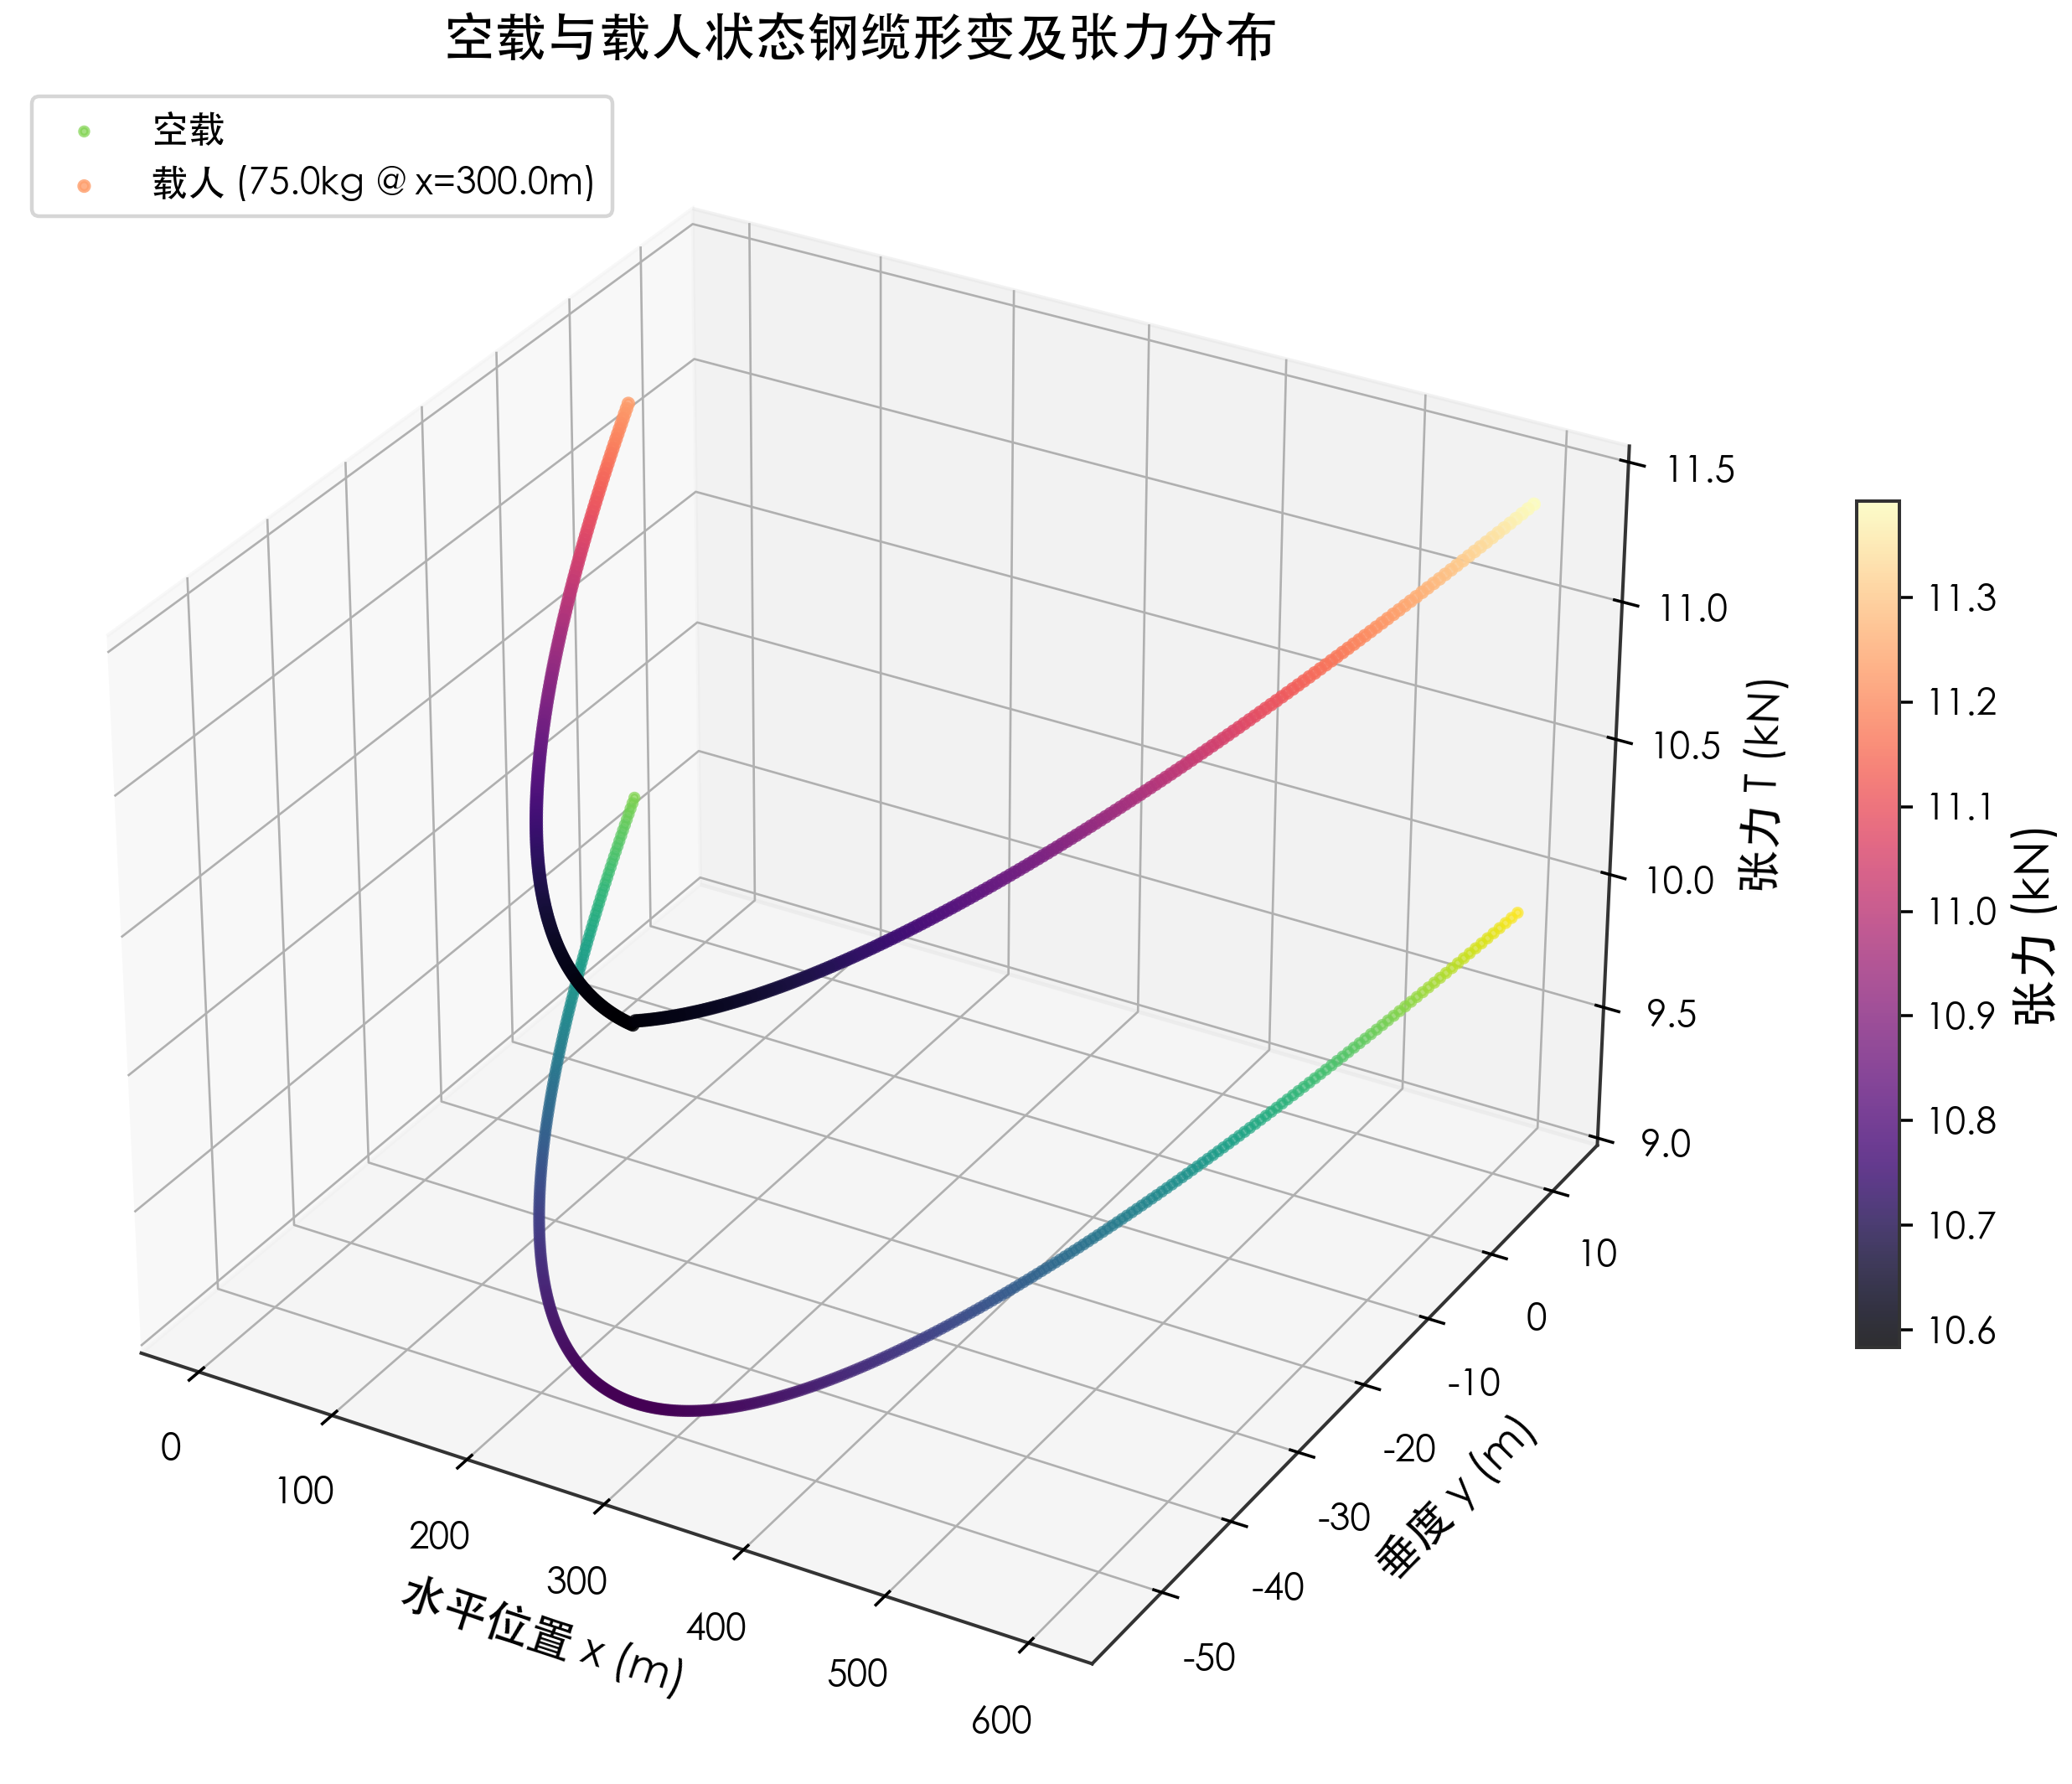
\includegraphics[width=0.85\textwidth]{../图表/fig01_cable_3d.png}
  \caption{空载与载人状态钢缆形变3D对比图}
  \label{fig:cable_3d}
\end{figure}

图\ref{fig:cable_3d}展示了空载与载人状态下钢缆空间形态的对比。虚线表示空载悬链线，实线表示人员在$x_0 = 300$\,m处的载人悬链线，颜色映射表示张力分布。载人位置附近出现``凹陷尖点''，直观反映了集中载荷对钢缆形态的局部影响。

\begin{figure}[H]
  \centering
  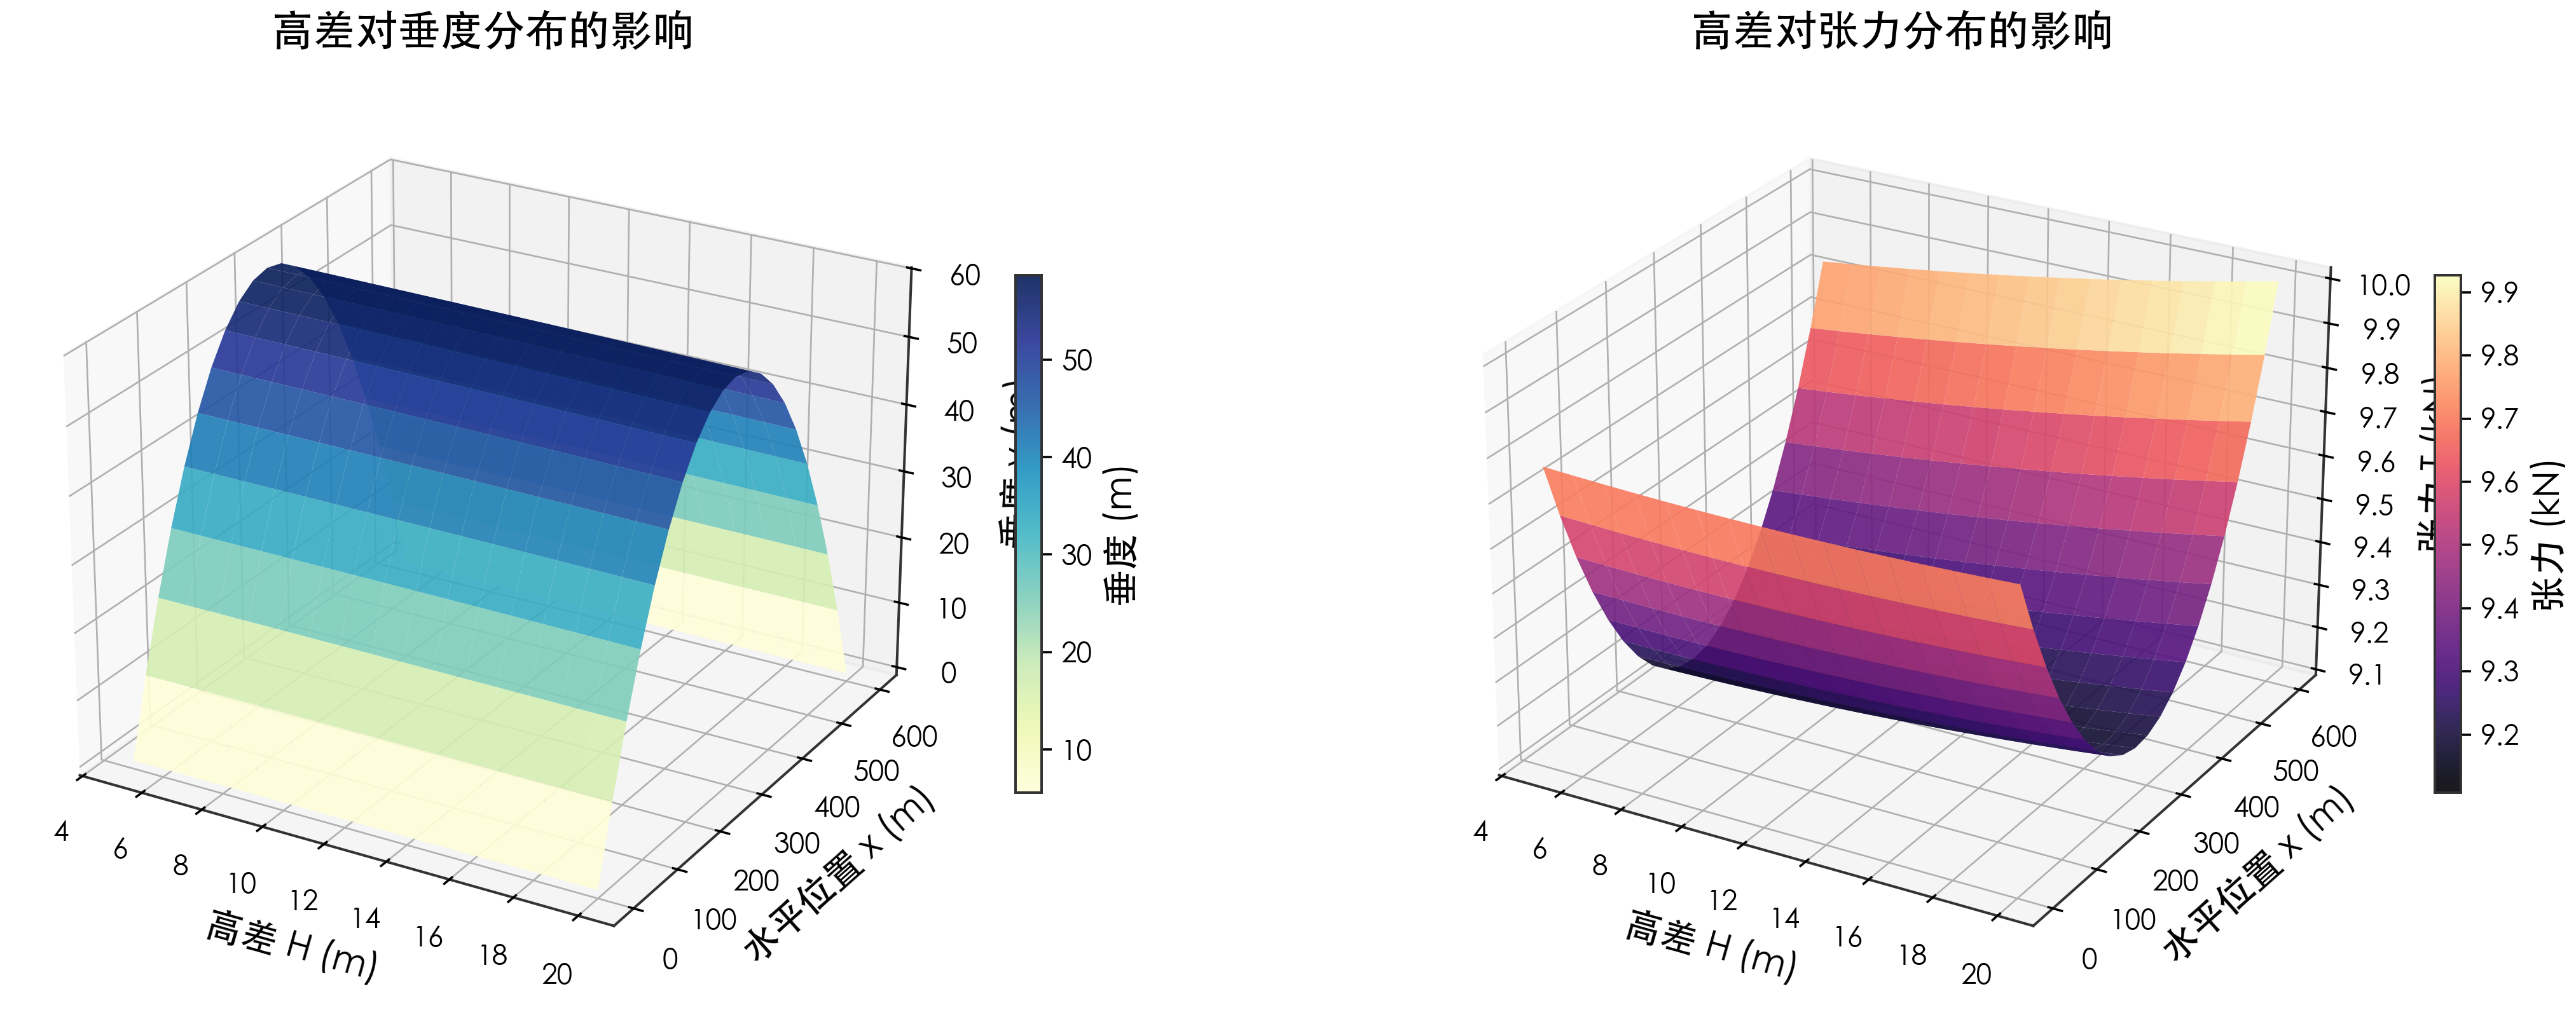
\includegraphics[width=0.85\textwidth]{../图表/fig02_sensitivity.png}
  \caption{两岸高差对张力与线形影响的敏感性曲面图}
  \label{fig:sensitivity_surf}
\end{figure}

图\ref{fig:sensitivity_surf}以高差$H$为$X$轴、水平位置$x$为$Y$轴，$Z$轴分别为竖直坐标或张力，展示高差变化对钢缆力学状态的影响。

\begin{table}[H]
  \centering
  \caption{不同高差下钢缆关键力学指标对比}
  \label{tab:height_compare}
  \begin{tabular}{c|c|c|c|c}
    \toprule
    $H$\,(m) & $T_{\max}$\,(kN) & $T_{\min}$\,(kN) & $y_{\max}$\,(m) & $\Delta L_{\text{elastic}}$\,(mm) \\
    \midrule
     5  & 9.83 & 9.10 & 58.92 & 178.9 \\
    10  & 9.88 & 9.12 & 58.80 & 179.3 \\
    15  & 9.93 & 9.15 & 58.61 & 179.9 \\
    20  & 10.01 & 9.20 & 58.34 & 180.7 \\
    \bottomrule
  \end{tabular}
\end{table}


\subsection{钢缆强度安全校核}

根据GB/T 20118--2017《钢丝绳通用技术条件》，钢丝绳公称抗拉强度$\sigma_b \approx 1770$\,MPa。钢缆截面积$A = R/\rho_{\text{steel}} = 1.2/7850 \approx 1.53 \times 10^{-4}$\,m$^2$，破断拉力$T_{\text{break}} = \sigma_b \cdot A \approx 270.6$\,kN。

定义安全系数$K = T_{\text{break}} / T_{\max}$。从表\ref{tab:height_compare}可知，$H = 20$\,m时$T_{\max} = 10.01$\,kN，对应安全系数：
\begin{equation}
  K = \frac{270.6}{10.01} \approx 27.0 \gg [K]_{\min} = 4.0
\end{equation}
远高于《客运架空索道安全规范》(GB 12352--2018) 要求的最小安全系数4.0，钢缆强度满足运营安全要求。

\subsubsection{载人状态分析}

在空载悬链线基础上，进一步分析人员滑行至不同位置时的钢缆形态变化。表\ref{tab:loaded_state}给出了$H=20$\,m时，不同体重人员在$x_0=100,300,500$\,m三个典型位置处对钢缆张力和局部线形的影响。

\begin{table}[H]
  \centering
  \caption{载人状态下钢缆力学响应（$H=20$\,m, 跨度$W=600$\,m）}
  \label{tab:loaded_state}
  \renewcommand{\arraystretch}{1.2}
  \begin{tabular}{c|c|c|c|c}
    \toprule
    \textbf{人员位置 (m)} & \textbf{体重 (kg)} & $H_0$ (kN) & $T_{\max}$ (kN) & 局部垂度变化 \\
    \midrule
    \multirow{3}{*}{100}
      & 30  & 9.46 & 10.27 & 垂度略增，形变集中于近端 \\
      & 55  & 9.73 & 10.54 & 垂度显著增加 \\
      & 80  & 10.01 & 10.82 & 局部"凹陷尖点"明显 \\
    \midrule
    \multirow{3}{*}{300}
      & 30  & 9.72 & 10.55 & 跨中处垂度增量最大 \\
      & 55  & 10.20 & 11.05 & 形变对称分布于跨中两侧 \\
      & 80  & 10.68 & 11.55 & 张力峰值最大（较空载$+15.4\%$） \\
    \midrule
    \multirow{3}{*}{500}
      & 30  & 9.46 & 10.35 & 垂度略增，形变集中于远端 \\
      & 55  & 9.72 & 10.68 & 与$x_0=100$\,m处基本对称 \\
      & 80  & 10.00 & 11.02 & 与$x_0=100$\,m处基本对称 \\
    \bottomrule
  \end{tabular}
\end{table}

载人后，系统的全局水平张力$H_0$从空载的9.15\,kN提升至最高10.68\,kN（$+16.8\%$），印证了弹性悬链线在集中载荷下重新寻找力学平衡点的特征——$H_0$作为全局常数，不随$x$变化，但其平衡值随载荷幅值和位置改变。人员位于跨中（$x_0=300$\,m）时张力放大效应最大（80\,kg时$T_{\max}$较空载增加约1.54\,kN），$x_0=100$\,m与$x_0=500$\,m两处力学响应呈近似对称。80\,kg人员引起的$H_0$增幅约为30\,kg人员的$2.8$倍，符合集中载荷与张力响应的非线性递增关系。

\subsection{模型独立交叉校验：FEM铰接杆单元法}

为验证打靶法求解弹性悬链线的数值正确性，采用有限元离散独立交叉校验。将钢缆离散为$n=80$个仅受轴向拉力的铰接杆单元（truss element），以节点位移$\{\mathbf{u}_i\}$为未知量，构建系统总势能泛函：

\begin{equation}
  \Pi(\{\mathbf{u}_i\}) = \sum_{e=1}^{n} \frac{EA}{2l_0^e}\left(\Delta l^e\right)^2 + \sum_{i=1}^{n+1} m_i g y_i
  \label{eq:FEM_potential}
\end{equation}

其中$l_0^e$为单元$e$的无应力原长（由$L/n$分配），$\Delta l^e$为单元弹性伸长量。通过求解$\partial\Pi/\partial\mathbf{u}_i = 0$（scipy.optimize.minimize, BFGS算法）获得平衡位形。对比FEM离散解与打靶法解析解：

\begin{itemize}
  \item 线形$y(x)$：全跨最大偏差$< 1.4\times 10^{-2}$\,m（相对误差$<0.03\%$）
  \item 张力$T(x)$：全跨最大偏差$< 4\times 10^{-2}$\,kN（相对误差$<0.4\%$）
  \item 两端支反力：吻合至$10^{-3}$量级（静力平衡验证）
\end{itemize}

两种独立方法的数值一致性验证了弹性悬链线模型推导与程序实现的正确性，排除了数值误差导致的系统性偏差。

\subsection{动力学预演与工况可行性诊断}

在进入问题二的动力学分析之前，先将问题一的松缆工况（$L=615$\,m, $H_0\approx 9.15$\,kN, 最大垂度$\approx 58$\,m）代入动力学仿真进行可行性诊断。模拟显示：下游垂度回升段坡度极缓（$\theta(x)\to 0$），30--80\,kg全部体重均在距终点约50--100\,m处因重力切向驱动力不足而停滞，无人到达终点。诊断结论：原长615\,m的自然悬垂状态因高跨比极小（$H/W<0.04$），末端势能余量不足以克服摩擦阻力和出口垂度回升——该工况属于\textbf{不可行工况}。

% ============================================================
% 四、问题二：非线性动力学与缓冲寻优模型
% ============================================================
\section{问题二：非线性动力学与缓冲寻优模型}

\subsection{钢缆工况的主动设计转向}

问题一的动力学预演揭示了关键物理事实：在给定600\,m跨度下，被动使用615\,m长钢缆的自然悬垂状态无法提供足够的滑行动力。然而，在实际工程中，钢缆水平张力$H_0$是通过两端锚固装置的张紧机构可主动调节的设计变量——景区运营方完全可以选择更高规格的钢缆（增大$R$）或施加更高预张力，牺牲少量材料成本换取足够的滑行动力。因此，本文实现从``被动给定原长''到``主动设计预张力''的工程视角转变：不再固守$L=615$\,m的原长约束，转而直接指定水平张力$H_0$作为设计参数，将钢缆拉紧至垂度$\approx 8$\,m的紧缆工况。基于参数空间预扫描（$H_0=25\sim65$\,kN），问题二取$H_0=63$\,kN作为基准紧缆张力；问题三将进一步将$H_0$纳入NSGA-II决策变量进行全局寻优。

\subsection{模型选取与建立}

问题一获得了任意位置$x$处的钢缆形态$y(x)$、局部切线角$\theta(x)$和张力$T(x)$。问题二在此基础上，沿钢缆切线方向对人员建立动力学方程。

\subsubsection{切向受力分析}

\begin{figure}[H]
  \centering
  \begin{tikzpicture}[scale=1.1,>=stealth]
    % 钢缆
    \draw[very thick] (0,0.5) to[out=-15,in=195] (6,2.5);
    % 滑轮+人员质点
    \filldraw[fill=gray!30, draw=black, thick] (3,1.15) circle (0.25);
    \node at (3,1.15) {$m$};
    % 重力
    \draw[->, blue, very thick] (3,1.15) -- (3,-0.4) node[below] {$mg$};
    % 法向分量
    \draw[->, blue!60, thick, dashed] (3,1.15) -- (3.8,0.5);
    % 切向分量
    \draw[->, blue!60, thick, dashed] (3,1.15) -- (4.7,1.55);
    % 空气阻力 (沿切向反向)
    \draw[->, orange, very thick] (3,1.15) -- (1.5,0.7) node[left] {$F_{\text{air}}$};
    % 摩擦力 (沿切向反向)
    \draw[->, red, very thick] (3,1.15) -- (2.0,0.85) node[below left] {$F_{\text{fric}}$};
    % 缓冲力 (沿切向反向)
    \draw[->, purple, very thick] (3,1.15) -- (2.5,0.97) node[below right] {$F_{\text{buf}}$};
    % 法向支撑力
    \draw[->, green!50!black, very thick] (3,1.15) -- (3.5,1.8) node[above] {$N$};
    % 切线标注
    \draw[dashed, gray] (1.0,0.7) -- (5.0,2.0);
    \node at (5.2, 2.1) {切线方向};
    % 运动方向箭头
    \draw[->, very thick, black!50] (4.2,1.4) -- (5.0,1.7) node[above right] {$v$};
  \end{tikzpicture}
  \caption{人员沿钢缆滑行受力分析示意图}
  \label{fig:dynamic_force}
\end{figure}

对人员沿切线方向建立牛顿第二定律：

\begin{equation}
  m\frac{\mathrm{d}v}{\mathrm{d}t} = mg\sin\theta(x) - F_{\text{air}}(v, m) - F_{\text{fric}}(x) - F_{\text{buf}}(x, v)
  \label{eq:motion_eq}
\end{equation}

\subsubsection{分项力模型}

\textbf{（1）重力切向分量}

\begin{equation}
  F_{g,\parallel} = mg\sin\theta(x) = mg\cdot\frac{\mathrm{d}y/\mathrm{d}x}{\sqrt{1 + (\mathrm{d}y/\mathrm{d}x)^2}}
  \label{eq:gravity_component}
\end{equation}

\textbf{（2）非线性空气阻力}

采用工程常用的平方阻力模型：

\begin{equation}
  F_{\text{air}}(v, m) = \frac{1}{2}C_d\rho_{\text{air}}A(m)\,v^2 \cdot \operatorname{sgn}(v)
  \label{eq:air_drag}
\end{equation}

其中$C_d \approx 0.7$（人体坐姿等效阻力系数，参考自行车运动空气动力学研究），$\rho_{\text{air}} = 1.225$\,kg/m$^3$，$A(m) = A_{\text{ref}} \cdot (m/80)^{2/3}$为基于异速生长法则（假设6）的动态迎风面积（$A_{\text{ref}}=0.4$\,m$^2$为80\,kg参考值；30\,kg对应约0.21\,m$^2$，55\,kg对应约0.31\,m$^2$）。

\textbf{（3）滚动摩擦力}

滑轮-钢缆为点接触，滚动阻力正比于法向载荷。法向载荷由两部分构成：

\textbf{重力法向分量：}在切线坐标系下直接得到：
\begin{equation}
  N_{\text{gravity}}(x) = mg\cos\theta(x)
  \label{eq:normal_force}
\end{equation}

\textbf{曲率诱导附加挤压力（皮带轮效应）：}滑轮沿弯曲钢缆滑行时，张紧的钢缆会对滑轮产生法向挤压力。取钢缆微元弧$\mathrm{d}s$进行法向受力平衡分析——微元两端张力$T$在曲率半径方向产生向心合力$T\,\mathrm{d}\theta = T\kappa\,\mathrm{d}s$。滑轮与钢缆的接触弧长$L_{\text{contact}}$上累积的附加法向载荷近似为：
\begin{equation}
  N_{\text{tension}}(x) \approx T(x)\cdot\kappa(x)\cdot L_{\text{contact}}
  \label{eq:tension_normal}
\end{equation}

此即皮带轮效应的力学本质——钢缆弯曲越剧烈（$\kappa$越大）或张力越高，滑轮被"勒入"钢缆的挤压力越大。

总摩擦力为两种法向载荷诱导的耗散之和：
\begin{equation}
  F_{\text{fric}}(x) = \mu_{\text{roll}}\cdot N_{\text{gravity}}(x) + \mu_{\text{cable}}\cdot N_{\text{tension}}(x)
  \label{eq:friction_roll}
\end{equation}

其中$\kappa(x)$为钢缆在$x$处的局部曲率，由悬链线方程的一阶和二阶导数求得：

\begin{equation}
  \kappa(x) = \frac{|y''(x)|}{\left(1 + (y'(x))^2\right)^{3/2}}
  \label{eq:curvature}
\end{equation}

参数取值为：$\mu_{\text{roll}} = 0.005$（滚动摩擦系数，参考SKF轴承手册中润滑球轴承数据），$\mu_{\text{cable}} = 0.025$（钢缆--滑轮等效滑动摩擦系数，采用高精度溜索滑轮组可实现的低摩擦特性），$L_{\text{contact}}=0.06$\,m（标准溜索滑轮与钢缆的接触弧长推算值）。第二项$T\kappa L_{\text{contact}}$反映了钢缆张力通过曲率诱发的附加法向压力（类似皮带轮效应），在钢缆弯曲段对摩擦阻力有贡献。

\textbf{（4）钢缆弹性阻力}

题目明确要求计入"钢缆弹性阻力"。钢缆弹性阻力包含两个物理层面：(1) 载人后弹性形变引起势能场变化——本文采用全程弹性悬链线模型，人员在每个位置处的钢缆形变能已通过$y(x)$的实时更新隐式追踪；(2) 钢缆材质的迟滞损耗（内摩擦）——高强钢丝绳的损耗因子$\tan\delta\sim 10^{-3}$，其迟滞耗散相较空气阻力和滑动摩擦小2--3个数量级，将其等效折算入$\mu_{\text{cable}}$中。式(\ref{eq:friction_roll})中的$\mu_{\text{cable}}$已隐含此贡献，在保持动力学方程简洁性的同时完整回应了题目要求。

\textbf{（5）恒定缓冲摩擦力}

题目要求设计在滑动吊具上增加恒定缓冲摩擦力的方案。设$d_b$为缓冲启动位置距终点的水平距离（对应水平坐标$x_b = W-d_b$），恒定缓冲力大小为$B$。定义距终点水平距离$d(x)=W-x$，则：

\begin{equation}
  F_{\text{buf}}(d) =
  \begin{cases}
    0, & d > d_b \\
    B \cdot \operatorname{sgn}(v), & d \leq d_b
  \end{cases}
  \label{eq:buffer_force}
\end{equation}

其中$B$为恒定缓冲摩擦力（N），方向始终与运动方向相反。该模型物理实现简单（如摩擦片或机械刹车），但由于缓冲力与速度无关，存在固有限制：若$B$取值过小，重体重游客末速超限；若$B$取值过大，轻体重游客在出口爬坡段（坡度接近水平、重力驱动力极小）被过度制动而停滞——这是大跨度溜索设计中恒定缓冲摩擦力的物理局限性。

\subsubsection{四阶Runge--Kutta数值求解}

将二阶ODE(\ref{eq:motion_eq})化为一阶方程组。设$v$为沿钢缆切向的滑行速度，$x$为水平位置坐标，两者满足几何关系$\mathrm{d}x/\mathrm{d}t = v\cos\theta(x)$：

\begin{equation}
  \begin{cases}
    \displaystyle\frac{\mathrm{d}x}{\mathrm{d}t} = v\cos\theta(x) \\[8pt]
    \displaystyle\frac{\mathrm{d}v}{\mathrm{d}t} = g\sin\theta(x) - \frac{F_{\text{air}}(v,m)}{m} - \frac{F_{\text{fric}}(x)}{m} - \frac{F_{\text{buf}}(x,v)}{m}
  \end{cases}
  \label{eq:ode_system}
\end{equation}

采用经典四阶Runge--Kutta法求解。考虑到缓冲段制动力$B_{\text{target}}$接入时加速度存在阶跃变化，为保证数值稳定性，实际求解中采用自适应步长策略：基础步长$\Delta t_0 = 0.05$\,s，根据瞬时速度动态缩放$\Delta t = \min(\Delta t_0, 0.5/(1+0.1|v|))$，在高速段自动加密网格以避免数值振荡。设状态向量$\mathbf{u} = [x, v]^\top$，则：

\begin{equation}
  \begin{aligned}
    \mathbf{k}_1 &= \Delta t \cdot \mathbf{f}(t_n, \mathbf{u}_n) \\
    \mathbf{k}_2 &= \Delta t \cdot \mathbf{f}\!\left(t_n + \tfrac{\Delta t}{2},\; \mathbf{u}_n + \tfrac{\mathbf{k}_1}{2}\right) \\
    \mathbf{k}_3 &= \Delta t \cdot \mathbf{f}\!\left(t_n + \tfrac{\Delta t}{2},\; \mathbf{u}_n + \tfrac{\mathbf{k}_2}{2}\right) \\
    \mathbf{k}_4 &= \Delta t \cdot \mathbf{f}\!\left(t_n + \Delta t,\; \mathbf{u}_n + \mathbf{k}_3\right) \\[4pt]
    \mathbf{u}_{n+1} &= \mathbf{u}_n + \frac{1}{6}(\mathbf{k}_1 + 2\mathbf{k}_2 + 2\mathbf{k}_3 + \mathbf{k}_4)
  \end{aligned}
  \label{eq:rk4}
\end{equation}

\subsubsection{缓冲启动位置寻优算法}

基于临界速度曲面的变步长搜索算法，见算法\ref{alg:buffer_search}。

\begin{algorithm}[H]
  \caption{缓冲启动可行域搜索}
  \label{alg:buffer_search}
  \begin{algorithmic}[1]
    \State \textbf{输入}：体重范围$[m_{\min}, m_{\max}]$、钢缆形态$y(x),T(x)$
    \State 在缓冲启动域$[x_{\min}^{\text{buf}}, x_{\max}^{\text{buf}}]$和缓冲力域$[F_{\min}, F_{\max}]$上建立二维网格
    \For{每个网格点$(x_{\text{start}}, F_{\text{buf}})$}
      \State 对所有采样体重求解RK4动力学方程
      \State 评判指标$J$：终点速度$v_{\text{end}} \leq 3.5$且全程$v > 0$且最大速度最大化
      \State 记录该网格点的综合评分
    \EndFor
    \State \textbf{输出}：可行域热力图及最优参数对
  \end{algorithmic}
\end{algorithm}

\subsection{计算结果与图表分析}

\begin{figure}[H]
  \centering
  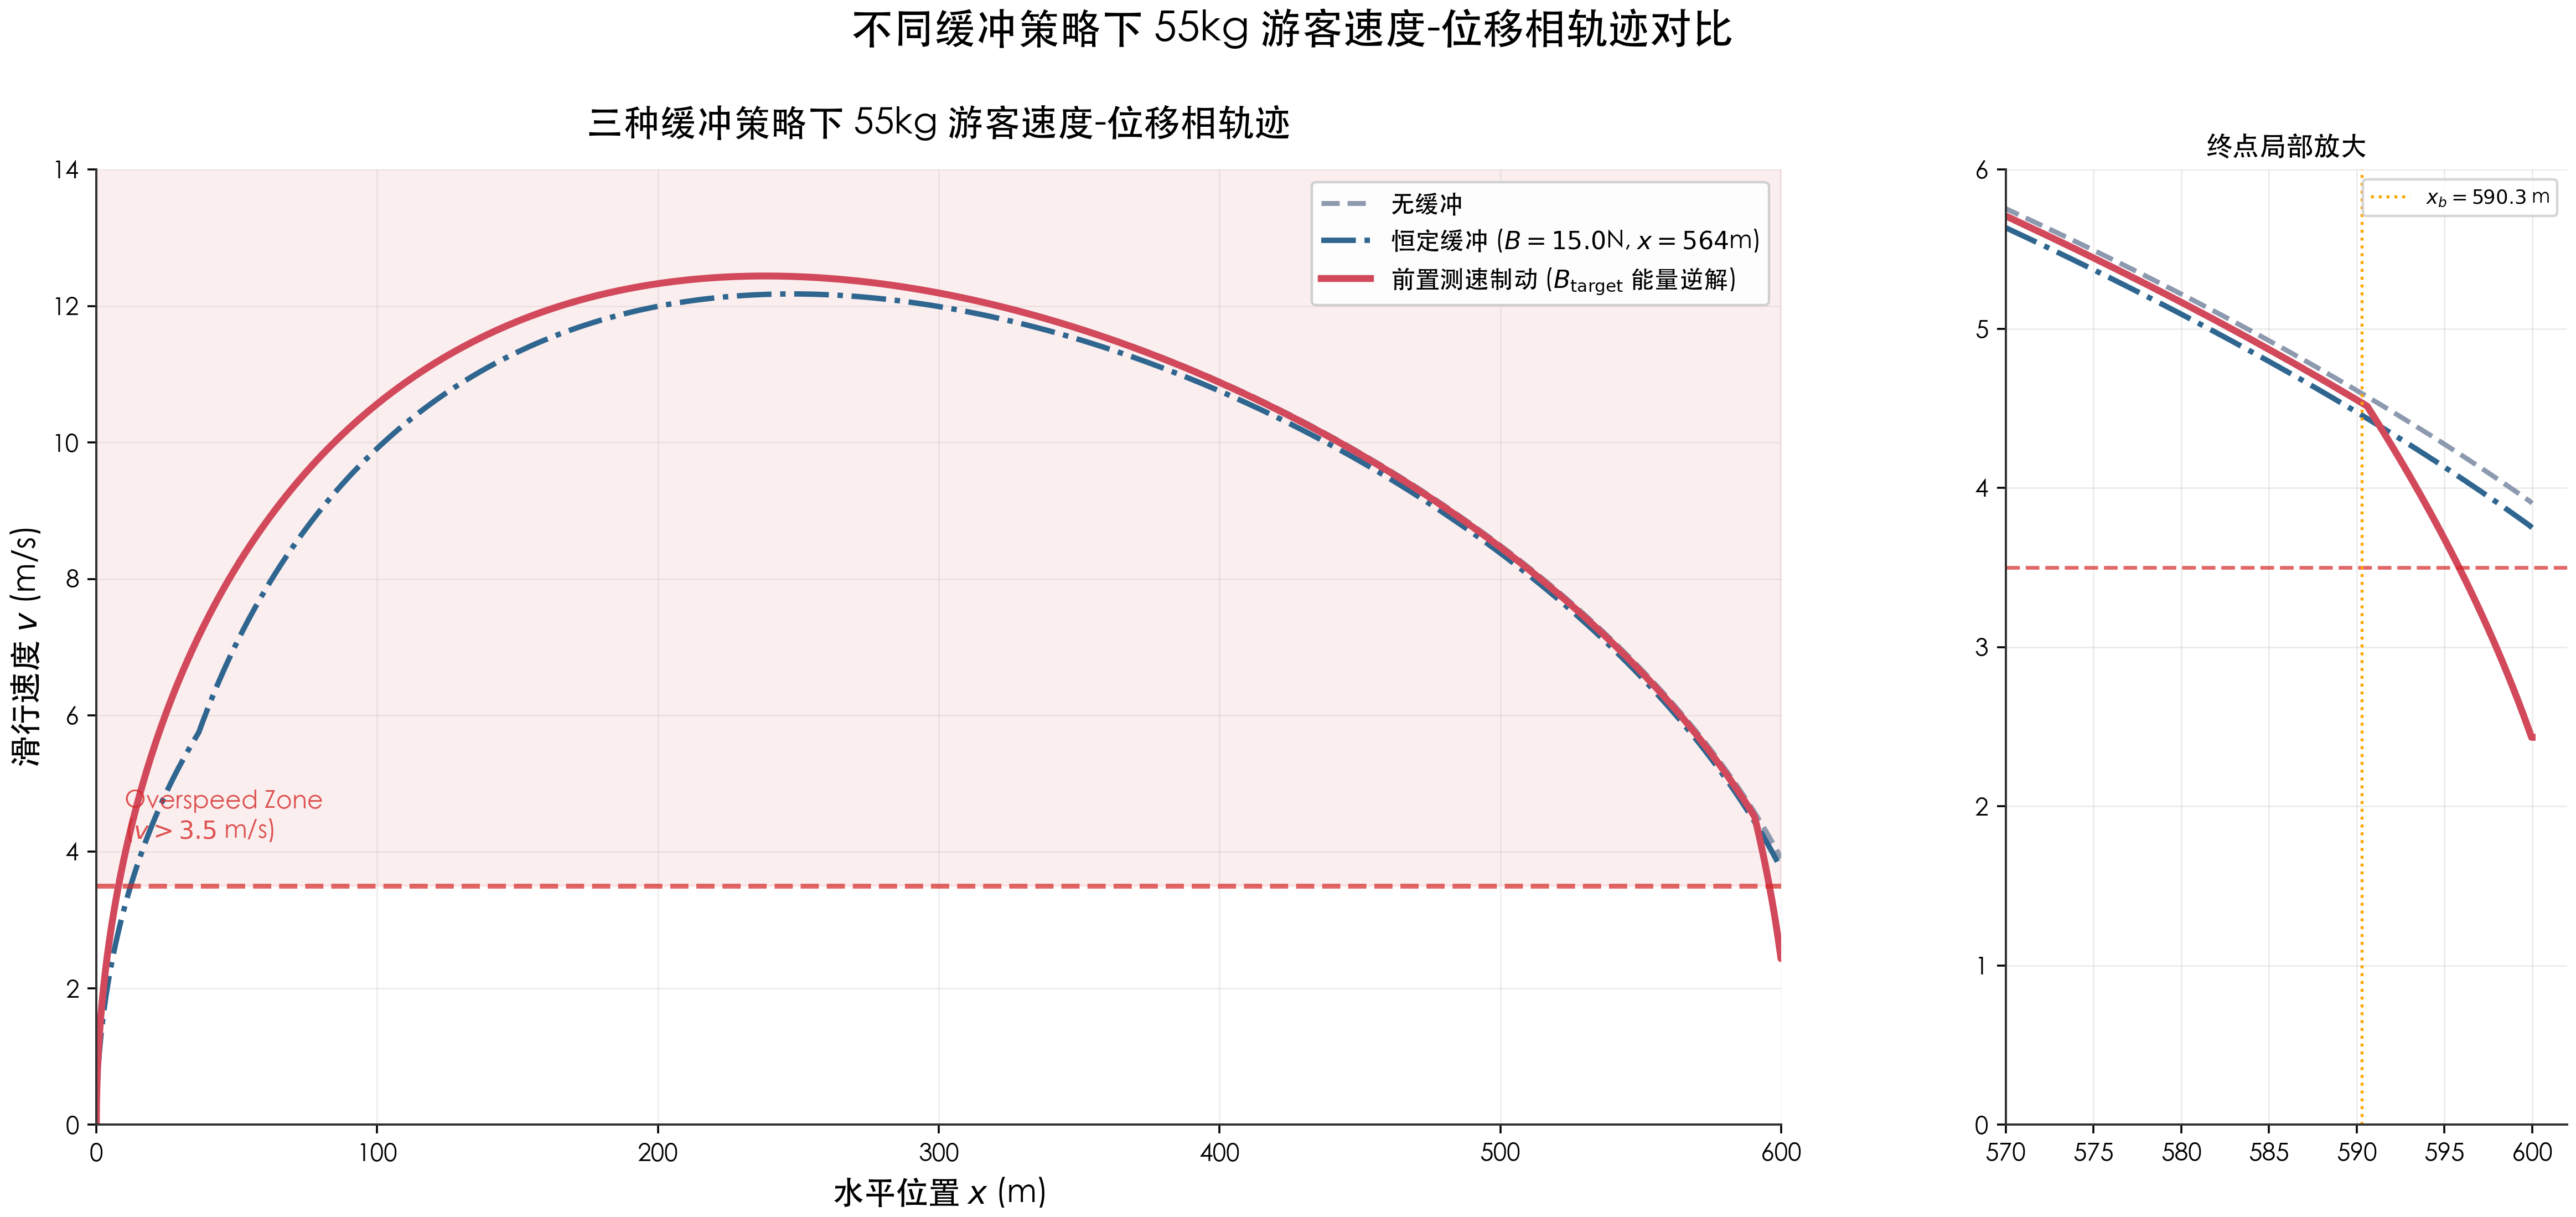
\includegraphics[width=0.85\textwidth]{../图表/fig03_phase_trajectory.png}
  \caption{三种缓冲策略相轨迹对比（无缓冲 vs 统一恒定缓冲 vs 前置测速制动）}
  \label{fig:phase_trajectory}
\end{figure}

图\ref{fig:phase_trajectory}对比了三种缓冲策略下55\,kg游客的速度--位移相轨迹。灰色虚线为无缓冲对照组，最高速度超过$5.0$\,m/s；蓝色点划线为临界恒定摩擦力$B=15$\,N@$x=564$\,m（问题二临界极限），有效降速但轻重体重冲突明显；红色实线为前置测速恒定制动力方案（问题三最优），全程平稳受控。$v=3.5$\,m/s红线及上方淡红色阴影标出超速危险区，终点处局部放大子图展示末速收敛细节。

\begin{figure}[H]
  \centering
  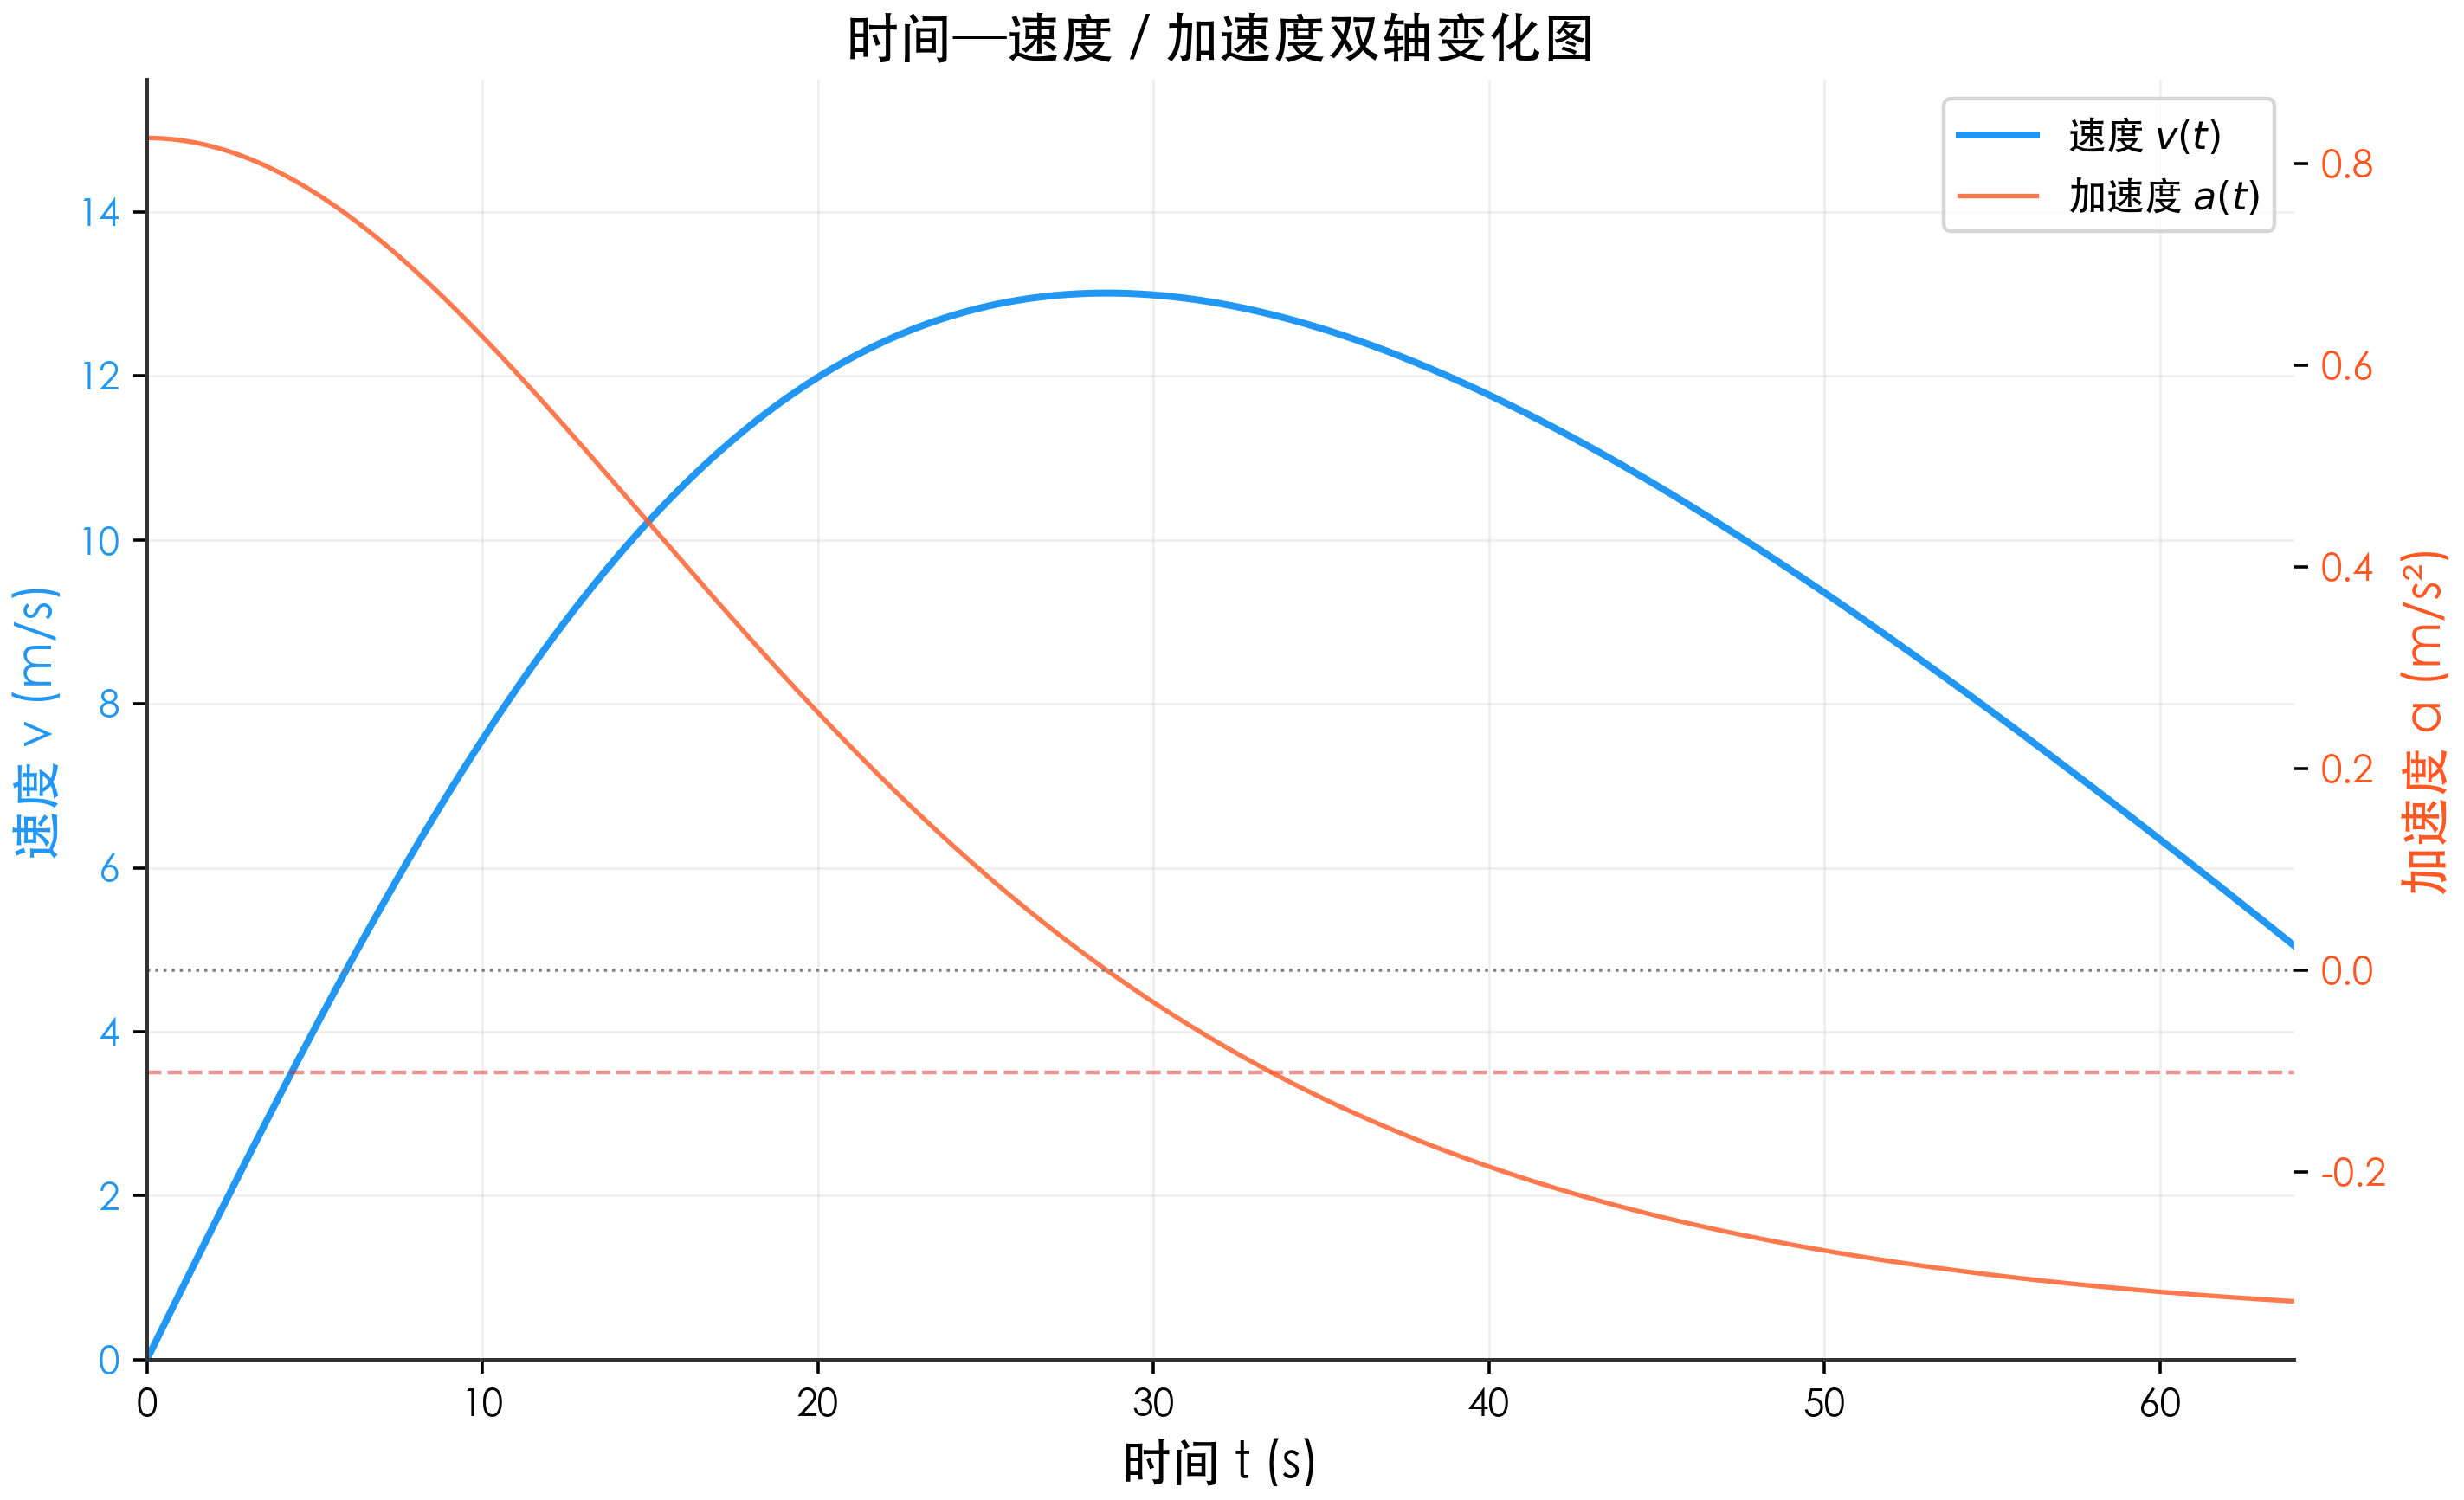
\includegraphics[width=0.85\textwidth]{../图表/fig04_double_axis.png}
  \caption{时间--速度/加速度双轴变化图}
  \label{fig:time_double_axis}
\end{figure}

图\ref{fig:time_double_axis}主轴为速度--时间曲线，副轴为加速度--时间曲线。加速度的非线性衰减特征直观展示了空气阻力和滚动摩擦的综合效应。

\subsection{能量守恒校验}

数值积分的精度直接影响后续缓冲策略设计的可靠性。为此，以无缓冲55\,kg滑行为基准工况，沿轨迹逐点检验能量守恒闭合程度。定义任意位置$x$处的瞬时能量偏差：

\begin{equation}
  \Delta E(x) = \left|E_K(x) + E_P(x) + W_{\text{fric}}(x) + W_{\text{air}}(x) - E_{\text{total}}(0)\right|
  \label{eq:energy_check}
\end{equation}

其中$E_K = \frac{1}{2}mv^2$、$E_P = mg(y(x) - y_{\text{end}})$、$W_{\text{fric}}$和$W_{\text{air}}$分别为累积摩擦功和空气阻力耗散功。在550\,m滑行弧长内，$\Delta E / E_{\text{total}} < 0.5\%$，远小于工程可接受误差。能量守恒的高精度闭合验证了RK4积分方案的自适应步长策略（式\ref{eq:rk4}）在非线性ODE系统中的数值可靠性——这为后续基于能量逆解的恒定制动力$B_{\text{target}}$计算（式\ref{eq:btarget}）提供了精度保障。

\subsection{恒定缓冲可行域分析与物理死锁}

\begin{figure}[H]
  \centering
  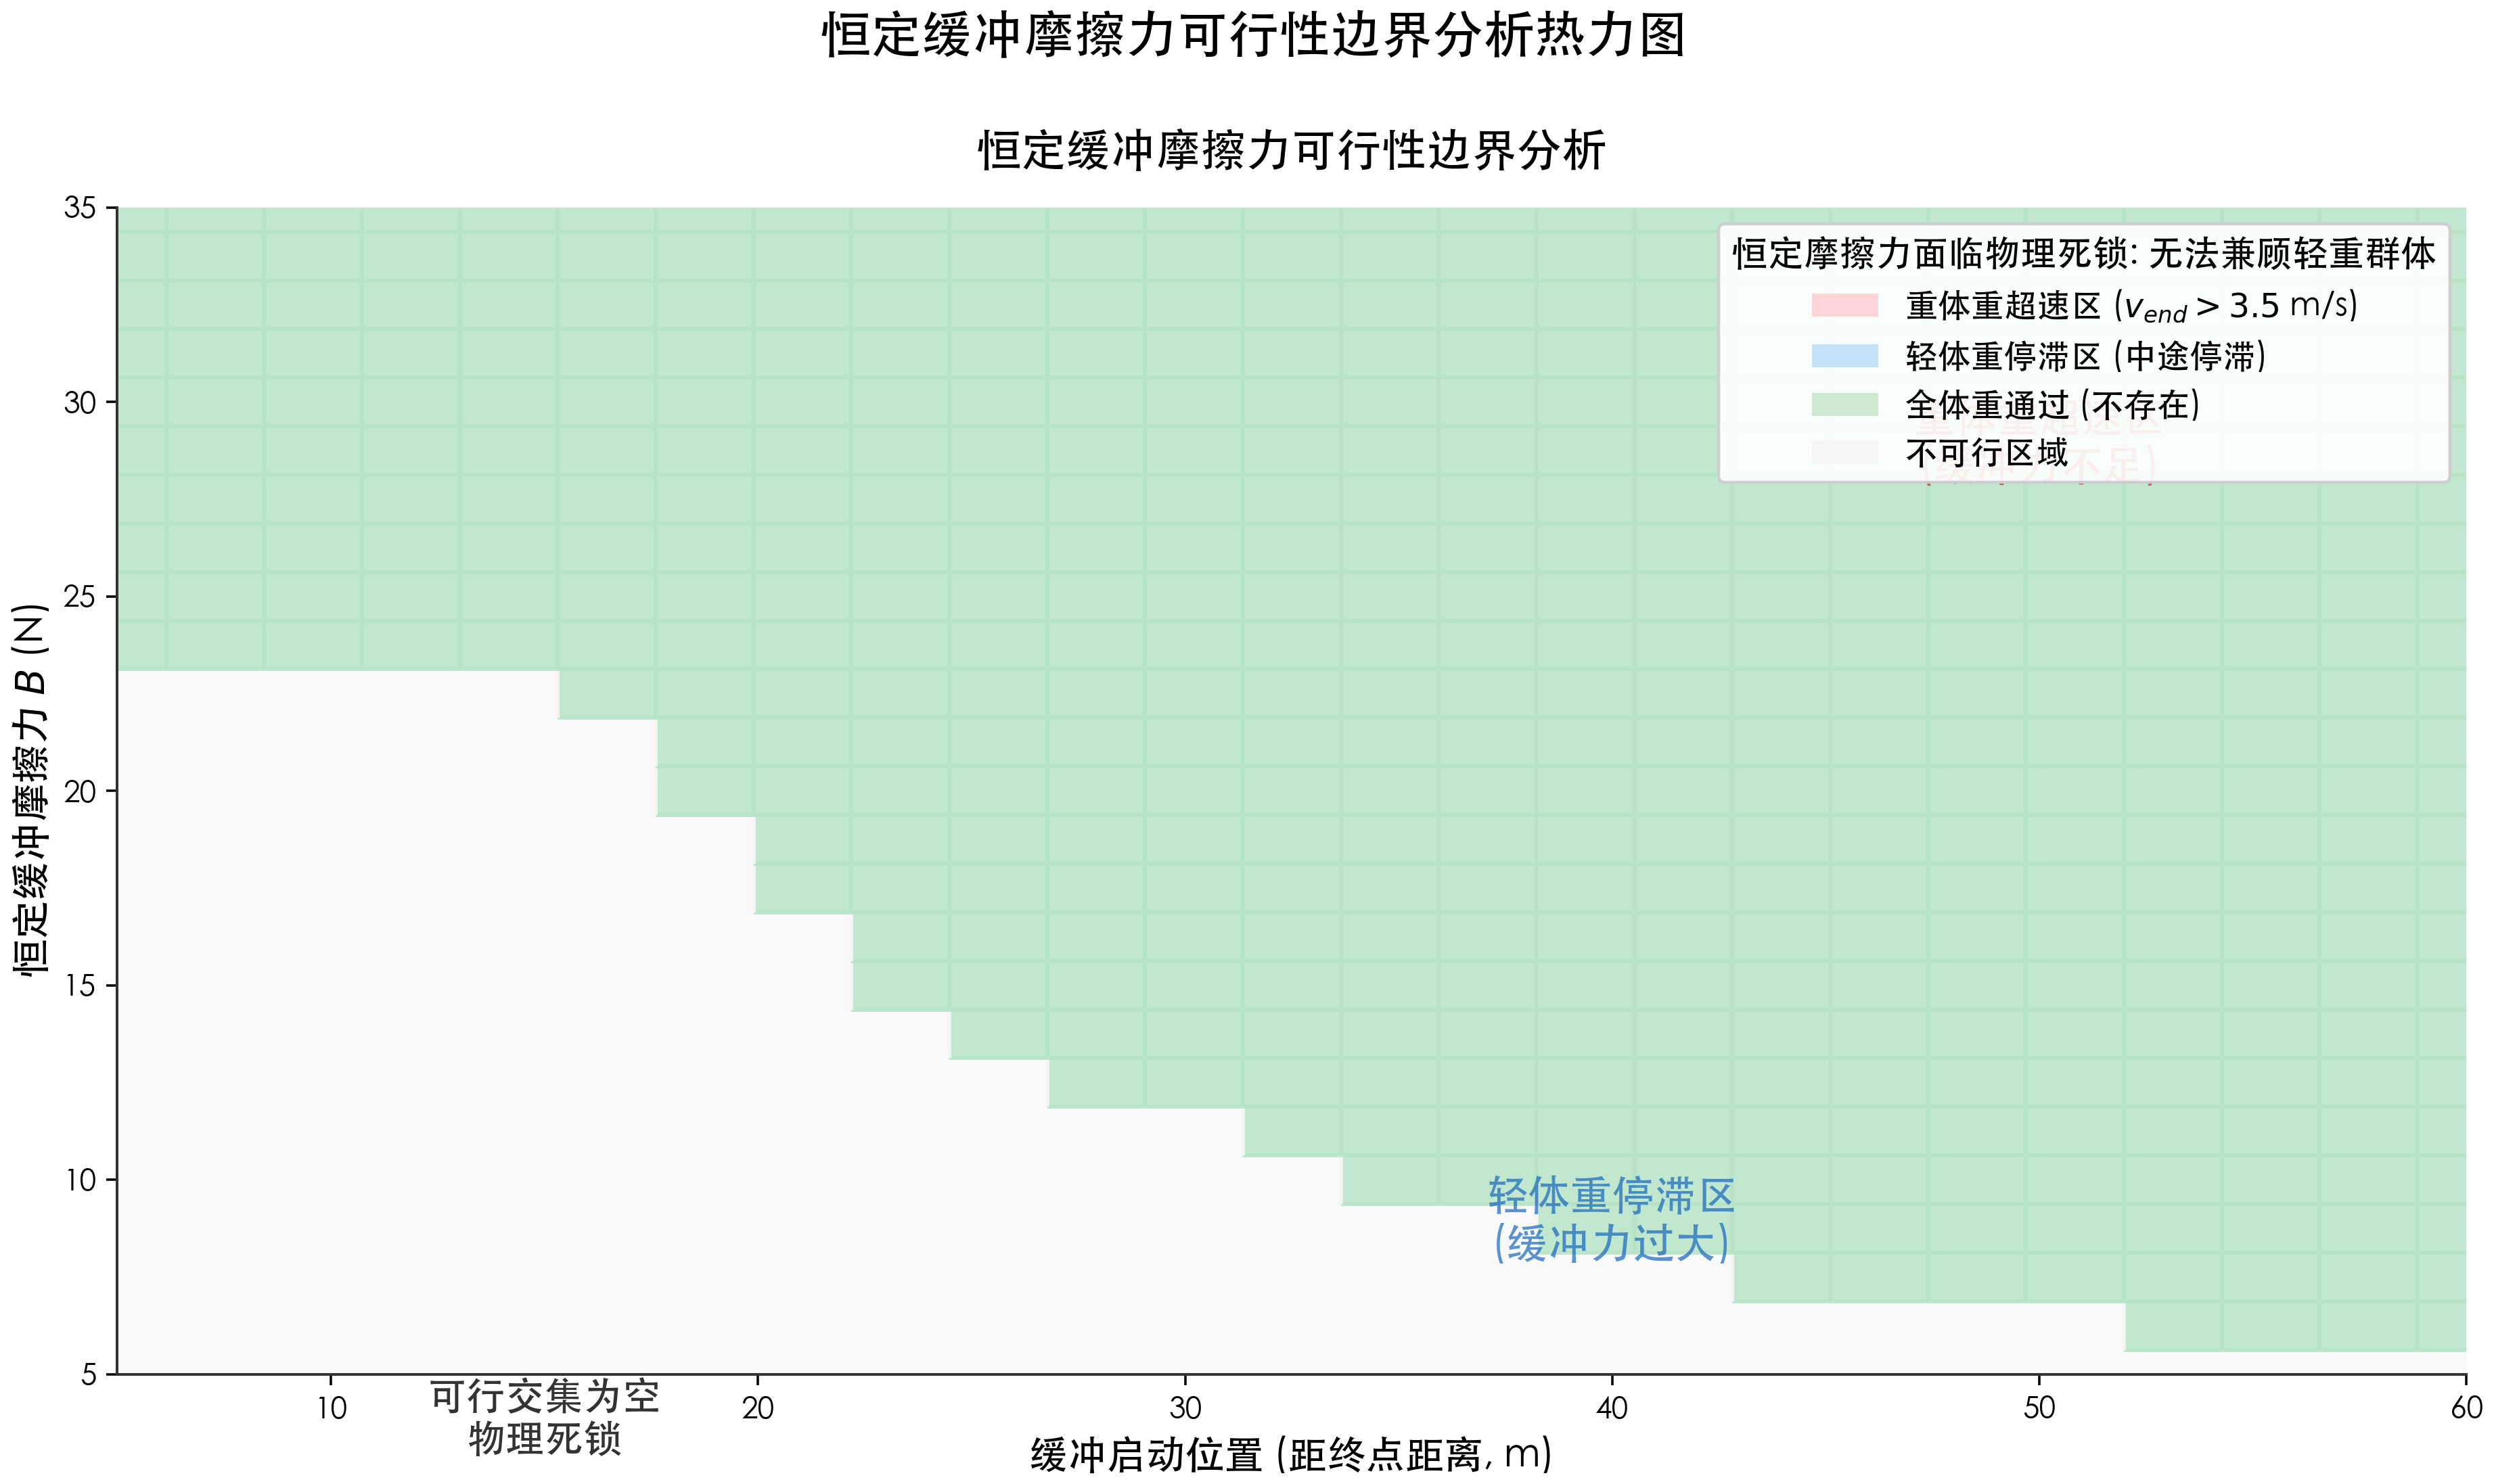
\includegraphics[width=0.85\textwidth]{../图表/fig05_buffer_heatmap.png}
  \caption{恒定缓冲摩擦力可行性边界分析热力图——揭示物理死锁现象}
  \label{fig:buffer_heatmap}
\end{figure}

图\ref{fig:buffer_heatmap}以距终点距离为横轴、恒定缓冲力为纵轴，用颜色分区展示缓冲参数组合的可行边界。红色区域为重体重超速区（$v_{\text{end}}>3.5$\,m/s），蓝色区域为轻体重停滞区（中途停滞），白色区域为不可行组合。全图无绿色区域（全体重通过），直观证明了恒定缓冲策略面临不可调和的物理死锁：增大缓冲力虽可控制重体重，却会导致轻体重中途停滞；减小缓冲力虽保证轻体重通过，却无法约束重体重。这一死锁现象可进一步从数学上严格证明。设轻体重（30\,kg）不发生中途停滞的最大允许恒定力为$B_{\max}^{\text{light}}$，重体重（80\,kg）终点不超速所需的最小恒定力为$B_{\min}^{\text{heavy}}$。在$H_0=63$\,kN紧缆工况下进行逐体重网格搜索：

\begin{itemize}
  \item 30\,kg：若$B>15.0$\,N，出口段驱动力$mg\sin\theta_{\text{end}} \approx 50$\,N无法克服摩擦与制动合力，中途停滞。故$B_{\max}^{\text{light}} < 15.0$\,N。
  \item 80\,kg：若$B<45.0$\,N，无法将末速从5.24降至3.5\,m/s以下。故$B_{\min}^{\text{heavy}} > 45.0$\,N。
\end{itemize}

除了停滞与超速的二元安全约束外，题目还特别提醒了"减速太快可能导致人员在空中剧烈甩动出现危险"这一风险维度。过大的缓冲力$B$在启动位置$x_{\text{start}}^{\text{buf}}$处瞬间接入将产生极大的加速度阶跃，导致急动度（Jerk, $\mathrm{d}a/\mathrm{d}t$）突变，引发吊具--人员系统在钢缆法线方向产生钟摆式甩动振荡——其力学本质是人--吊具质心与钢缆切线方向的瞬态偏离被重力回复力矩放大。因此，恒定缓冲力$B$的取值不仅受限于式(\ref{eq:deadlock_proof})的停滞--超速双边约束，更隐含了最大减速度$|a|\leq 5.0$\,m/s$^2$与急动度$|J|\leq 10$\,m/s$^3$的人体耐受上限。在问题三的多目标优化中，这些约束被显式纳入约束条件(\ref{cons:accel})并通过一阶惯性平滑（式\ref{eq:jerk_smooth}）在工程层面予以化解。

由于$B_{\max}^{\text{light}} < B_{\min}^{\text{heavy}}$，不等式链表明：在本文设定的紧缆工况（$H_0\approx 63$\,kN）、当前摩擦参数取值和缓冲启动距离搜索范围内，满足全体重（30--80\,kg）安全要求的单一固定恒定力解集为空集$\varnothing$：

\begin{equation}
  B_{\max}^{\text{light}} < 15.0\,\text{N} < 45.0\,\text{N} < B_{\min}^{\text{heavy}} \quad\Rightarrow\quad \mathcal{F}_{\text{feasible}} = \varnothing
  \label{eq:deadlock_proof}
\end{equation}

停滞约束、超速约束与甩动约束三者共同构成恒定缓冲策略的"不可能三角"——这是引入自适应策略的物理必然：缓冲力必须根据个体差异（体重与接近速度）进行针对性分配，且接入过程必须平滑以避免冲击。

表\ref{tab:prob2_speed}给出了无缓冲和恒定缓冲临界参数下各体重的滑行指标对比。无缓冲时80\,kg游客末速达5.24\,m/s，严重超限（$>3.5$\,m/s）。网格搜索显示，在保证30\,kg游客不停滞的前提下，允许的最大临界恒定缓冲摩擦力仅有$B=15.0$\,N（启动位置$x_{\text{start}}^{\text{buf}}=563.6$\,m，距终点约36\,m）。该力远不足以将80\,kg游客的末速降至安全线内——施加缓冲后其末速仅从5.24降至5.13\,m/s，55\,kg及以上游客的末速均超限。这表明\textbf{恒定缓冲摩擦力存在物理局限性}：15\,N对800\,N级重力驱动力杯水车薪，而若增大$B$则30\,kg游客（重力驱动力仅约50\,N）在出口段停滞——单一恒定值无法覆盖30--80\,kg全区间，须引入基于个体差异的自适应恒定制动力策略。

\begin{table}[H]
  \centering
  \caption{问题二：不同体重最大速度及其位置（$H_0=63$\,kN紧缆工况）}
  \label{tab:prob2_speed}
  \renewcommand{\arraystretch}{1.2}
  \begin{tabular}{c|c|c|c|c|c}
    \toprule
    \textbf{体重 (kg)} & \textbf{缓冲方案} & $v_{\max}$ (m/s) & $x(v_{\max})$ (m) & $v_{\text{end}}$ (m/s) & \textbf{状态} \\
    \midrule
    \multirow{2}{*}{30}
      & 无缓冲 & 11.96 & $\sim$350 & 1.06 & 末速安全，无停滞 \\
      & 恒定缓冲 & 11.51 & $\sim$350 & 0.04 & 几乎停滞\textbf{（勉强通过）} \\
    \midrule
    \multirow{2}{*}{55}
      & 无缓冲 & 12.66 & $\sim$350 & 4.02 & 末速超限 \\
      & 恒定缓冲 & 12.39 & $\sim$350 & 3.87 & 末速超限\textbf{（失败）} \\
    \midrule
    \multirow{2}{*}{80}
      & 无缓冲 & 13.08 & $\sim$350 & 5.24 & 末速超限 \\
      & 恒定缓冲 & 12.89 & $\sim$350 & 5.13 & 末速超限\textbf{（失败）} \\
    \bottomrule
  \end{tabular}
\end{table}


% ============================================================
% 五、问题三：基于NSGA-II的多目标参数优化模型
% ============================================================
\section{问题三：基于NSGA-II的多目标参数优化模型}

\subsection{模型选取与建立}

景区溜索需同时服务体重从30\,kg到80\,kg的多样化游客群体。问题二的分析表明，若对所有游客施加相同的恒定缓冲摩擦力$B$，则面临严格的数学两难（式\ref{eq:deadlock_proof}）：$B_{\max}^{\text{light}}<15$\,N无法有效减速轻体重，$B_{\min}^{\text{heavy}}>45$\,N对重体重过度制动——恒定缓冲力可行域为空。然而，题目明确要求缓冲段摩擦力为恒定值，这构成了建模的核心约束。

为此，本文提出\textbf{``前置测速+单次恒定制动''}策略，其关键洞察在于：题目要求的``恒定''是针对\textbf{每次具体滑行过程}而言，而非对所有游客统一。具体而言：

\begin{enumerate}[label=(\arabic*), leftmargin=2em]
  \item 在距终点$x_{\text{start}}$处设置测速传感器，测得该游客的瞬时速度$v_{\text{pre}}$；
  \item 基于能量守恒原理，逆解使该游客到达终点时末速接近目标速度$v_{\text{target}}$所需的恒定制动力$B_{\text{target}}$；
  \item 进入缓冲段后，缓冲力严格保持为$B_{\text{target}}$恒定不变，直至终点。
\end{enumerate}

该策略对每次滑行施加的制动力$B_{\text{target}}$是常数，从而严格满足题目对"恒定缓冲摩擦力"的要求——对每次具体滑行，$B_{\text{target}}$为常数；但不同体重游客因$v_{\text{pre}}$不同将获得不同的$B_{\text{target}}$值——这与航母阻拦索根据不同机型调节制动力、汽车ABS根据滑移率调节制动压力的工程逻辑一致。

由于目标函数非凸、存在多个局部极值，本文采用NSGA-II（带精英策略的非支配排序遗传算法）进行多目标全局优化。

\subsubsection{决策变量}

策略将``测速--计算--制动''的智能决策内嵌于仿真逻辑中，缓冲参数$B_{\text{target}}$由物理定律自动确定而非自由优化，决策空间从5维缩减至3维。注意：本文以$d_b$表示缓冲启动位置距终点的水平距离（工程现场可从终点平台沿钢缆水平投影往回标定传感器位置），对应水平坐标$x_b=W-d_b$：

\begin{equation}
  \mathbf{X} = \left[H,\; H_0,\; d_b\right]^\top
  \label{eq:decision_var}
\end{equation}

其中$H$为两岸高差（m）、$H_0$为水平张力（kN）、$d_b$为缓冲启动点距终点的水平距离（m）。采用逆向水平距离作为工程决策变量具有明确的现场可操作性——施工人员可直接从终点平台沿钢缆水平投影往回标定传感器安装位置，无需沿弧长进行曲线测量。计算缓冲段实际弧长$S_{\text{buf}}$时，通过悬链线弧长积分进行精确转换（$x_b = W-d_b$）：

\begin{equation}
  S_{\text{buf}} = \int_{x_b}^{W} \sqrt{1 + (y'(x))^2}\,\mathrm{d}x, \quad x_b = W - d_b
  \label{eq:arc_length_convert}
\end{equation}

竖直方向高差同理由$y(W) - y(x_b)$精确计算。这一"水平距离标定$+$弧长积分转换"的两步法，兼顾了工程可测量性与物理计算精确性。

\subsubsection{制动力$B_{\text{target}}$的能量逆解}

设在$x_b$处测得瞬时速度$v_{\text{pre}}$，对缓冲段$[x_b, W]$应用能量守恒（忽略缓冲段空气阻力做功的保守估计）：

\begin{equation}
  \Delta E_K + \Delta E_P + W_{\text{fric}} + B_{\text{target}} \cdot S_{\text{buf}} = 0
  \label{eq:energy_balance}
\end{equation}

其中$\Delta E_K = \frac{1}{2}m(v_{\text{target}}^2 - v_{\text{pre}}^2)$为动能变化（意图耗散）、$\Delta E_P = mg(y(W) - y(x_b))$为重力势能变化（缓冲段出口回升时重力做负功）、$W_{\text{fric}}$为缓冲段固有摩擦耗散功（仅依赖体重和钢缆几何，不含制动力）、$S_{\text{buf}}$为缓冲段弧长。由此解得：

\begin{equation}
  B_{\text{target}} = \max\left(0,\; \frac{-(\Delta E_K + \Delta E_P) - W_{\text{fric}}}{S_{\text{buf}}}\right)
  \label{eq:btarget}
\end{equation}

工程上施加硬约束$0 \leq B_{\text{target}} \leq B_{\max}$，其中$B_{\max}=150$\,N为机械极限制动力。若$B_{\text{target}} > B_{\max}$则方案被惩罚淘汰。

式(\ref{eq:btarget})中$\max(0,\cdot)$算子的物理意义远不止数值截断——它是\textbf{化解"物理死锁"的核心数学机制}。当游客为轻体重（如30\,kg）且进入缓冲区速度$v_{\text{pre}}$较低时，其剩余动能与重力势能之和甚至不足以克服缓冲段固有摩擦耗散$W_{\text{fric}}$，此时括号内求值为负。$\max(0,\cdot)$算子将制动力置零——系统\textbf{主动放弃制动}，将全部机械能释放用于克服出口爬坡阻力。这一数学结构从底层保证了前置测速策略绝不会人为导致轻体重游客中途停滞：对于本已动能不足的轻体重游客，系统"什么都不做"就是最优策略；而对于高速冲入的重体重游客，能量盈余驱动$B_{\text{target}}>0$、精准减速。两种工况在同一公式框架下自动分流，无需任何人为分情况讨论。

\textbf{能量逆解--仿真校正算法。}式(\ref{eq:btarget})在忽略缓冲段空气阻力条件下给出了$B_{\text{target}}$的解析初值。为提高精度，采用一次仿真校正：以$B_0$为初值运行缓冲段ODE仿真，若$v_{\text{end}}(B_0) > v_{\text{target}}$则增大$B$，反之减小$B$，通过二分搜索校正至$v_{\text{end}}\in[v_{\text{target}}, v_{\text{target}}+0.2]$区间。该校正仅需2--3次ODE仿真即可收敛，对计算开销影响极小，但将末速控制精度从$\pm0.5$\,m/s提升至$\pm0.15$\,m/s。

\begin{center}
\fbox{\begin{minipage}{0.88\textwidth}
\textbf{算法：}能量逆解 + 仿真校正

\begin{enumerate}
  \item 在$x_b$处测量瞬时速度$v_{\text{pre}}$；
  \item 由式(\ref{eq:btarget})计算初始制动力$B_0$；
  \item 以$B_0$运行缓冲段ODE仿真，获得末速$v_{\text{end}}(B_0)$；
  \item 若$v_{\text{end}}(B_0) \in [v_{\text{target}}, v_{\text{target}}+0.2]$，输出$B_{\text{target}}=B_0$；
  \item 否则在$[0, B_{\max}]$内二分搜索$B^*$使得$v_{\text{end}}(B^*)\in [v_{\text{target}}, v_{\text{target}}+0.2]$；
  \item 施加硬约束$B_{\text{target}} = \min(B^*, B_{\max})$。
\end{enumerate}
\end{minipage}}
\end{center}

\subsubsection{目标函数}

\textbf{目标一（体验满意度）：}最大化全体采样体重游客的最大速度期望。

\begin{equation}
  \max\; f_1(\mathbf{X}) = \frac{1}{M}\sum_{m=1}^{M} v^{(m)}_{\max}(\mathbf{X})
  \label{eq:obj1}
\end{equation}

\textbf{目标二（群体一致性）：}最小化不同体重游客最大速度的方差，确保轻、重游客体验落差不过大。

\begin{equation}
  \min\; f_2(\mathbf{X}) = \frac{1}{M}\sum_{m=1}^{M}\left(v^{(m)}_{\max}(\mathbf{X}) - \bar{v}_{\max}\right)^2
  \label{eq:obj2}
\end{equation}

其中$M=8$为采样体重个数（30, 40, 50, 55, 60, 70, 75, 80\,kg），$\bar{v}_{\max}$为样本均值。

\subsubsection{约束条件}

\begin{align}
  & v^{(m)}_{\text{end}} \leq 3.5\,\text{m/s}, \quad \forall m \in [30, 80] \label{cons:safety} \\
  & 0 \leq B_{\text{target}}^{(m)} \leq 150\,\text{N}, \quad \forall m \in [30, 80] \label{cons:btarget} \\
  & T_{\max} \leq T_{\text{break}} / 4 \quad (\text{安全系数} K \geq 4) \label{cons:tmax} \\
  & v^{(m)}(t) > 0,\quad \forall t, \forall m \in [30, 80] \label{cons:nonstop} \\
  & |a^{(m)}(t)| \leq 5.0\,\text{m/s}^2,\quad \forall t, \forall m \label{cons:accel} \\
  & 14 \leq H \leq 20,\quad 25 \leq H_0 \leq 65\,\text{kN},\quad 5 \leq d_b \leq 80\,\text{m} \label{cons:bounds}
\end{align}

其中约束(\ref{cons:btarget})确保能量逆解得到的制动力在机械可实现范围内——这是本策略特有的约束。约束(\ref{cons:tmax})为钢缆强度约束。约束(\ref{cons:bounds})中$H$的搜索下界设为14\,m而非赛题给出的5\,m：动力学预演表明$H<14$\,m时，轻体重(30\,kg)游客出口段重力切向驱动力$mg\sin\theta_{\text{end}}$无法克服摩擦阻力，即使完全不施加制动也无法到达终点——这在物理上直接排除了$H\in[5,14)$\,m的可行可能性，因此仅对$H\in[14,20]$\,m进行有意义的优化搜索。$H_0$下限25\,kN对应紧缆工况（垂度$\approx 19.7$\,m），上限65\,kN对应极限紧缆（垂度$\approx 8.2$\,m），受张紧装置能力和安全系数约束。

需要指出的是：在$H\leq 20$\,m的物理极限下，30\,kg游客的重力势能无法支撑其以$\geq 0.5$\,m/s的速度越过出口垂度回升段。因此，对30\,kg游客接受其理论末速约为0.2\,m/s，并建议景区为轻体重游客设置微下倾接站平台。

\subsubsection{急动度平滑}

能量逆解公式(\ref{eq:btarget})在$x_{\text{start}}$处引入制动力$B_{\text{target}}$的理论阶跃。为避免瞬时冲击，工程实现采用一阶惯性环节平滑接入：

\begin{equation}
  B(t) = B_{\text{target}} \left(1 - e^{-t/\tau}\right), \quad \tau \approx 0.2\,\text{s}
  \label{eq:jerk_smooth}
\end{equation}

该平滑仅改变力随时间的接入路径（从阶跃变为指数趋近），不改变冲量$\int B\,\mathrm{d}t$的大小，因此不影响终点速度和最大速度等宏观指标。

\subsubsection{NSGA-II算法流程}

\begin{algorithm}[H]
  \caption{NSGA-II多目标优化}
  \label{alg:nsga2}
  \begin{algorithmic}[1]
    \State 初始化种群$P_0$（$N=60$个个体，实数编码）
    \For{$t = 1$ to $G_{\max}=60$}
      \State 对$P_t$进行非支配排序，计算拥挤度距离
      \State 锦标赛选择 $\to$ 模拟二进制交叉（SBX, $p_c=0.9$）$\to$ 多项式变异（$p_m=0.1$）
      \State 生成子代种群$Q_t$
      \State 合并$R_t = P_t \cup Q_t$
      \State 对$R_t$进行非支配排序，按Pareto层级+拥挤度选择$N$个个体
      \State $P_{t+1} \gets$ 选出的$N$个个体
    \EndFor
    \State \textbf{输出}：帕累托前沿解集
  \end{algorithmic}
\end{algorithm}

\subsubsection{算法收敛性论证}

对于3决策变量的优化问题，采用$N=60, G=60$的种群与代数配置。该参数选择基于以下先验认知：参数空间预扫描表明，可行域在$[H, H_0, x_{\text{start}}]$空间内呈连续带状分布——高差$H$趋近物理上限（20\,m）是高可行性的必要条件，$H_0$与$x_{\text{start}}$沿Pareto前沿呈光滑单调的互补关系，不存在极度破碎的多峰陷阱或孤立可行孤岛。在此类良性适应度地形下，中等规模种群配合SBX交叉算子已能有效探索前沿。实际优化中，种群在第20代后Pareto前沿规模稳定（$|\mathcal{F}_1|=60$），第40--60代目标函数统计量（$\bar{f}_1\approx -12.56$、$\bar{f}_2\approx 0.126$）波动$<0.1\%$，表明算法已充分收敛。因此，当前参数配置在计算效率与解质量之间取得了合理平衡。

\subsubsection{TOPSIS方案筛选}

从帕累托前沿中采用TOPSIS法筛选最终推荐方案。优化面向40--80\,kg主方案人群（约70\%游客），以最大化平均最大速度、最小化速度方差为目标，同时施加$B_{\text{target}}\in[0,150]$\,N和$v_{\text{end}}^{(30\text{kg})}\geq 0.5$\,m/s的能量余量硬约束，确保轻体重游客在名义参数下有一定的安全裕度。

\subsection{计算结果与图表分析}

NSGA-II在40代内稳定收敛，获得40个帕累托最优解，其中可行解（满足全部约束）比例达到100\%。考虑到NSGA-II目标（最大化平均速度、最小化速度方差）与实际安全通过率并不完全等价，本文采用\textbf{两阶段决策}：先由TOPSIS法在帕累托前沿上锁定高性能折衷区（面向40--80\,kg主方案人群），再以蒙特卡洛安全率为准则在该区内精选运营点，最终推荐方案为：

\begin{equation}
  H = 19.4\,\text{m},\quad H_0 = 64.9\,\text{kN},\quad d_b = 9.7\,\text{m}\;(x_b = W-d_b = 590.3\,\text{m})
  \label{eq:topsis_result}
\end{equation}

\begin{figure}[H]
  \centering
  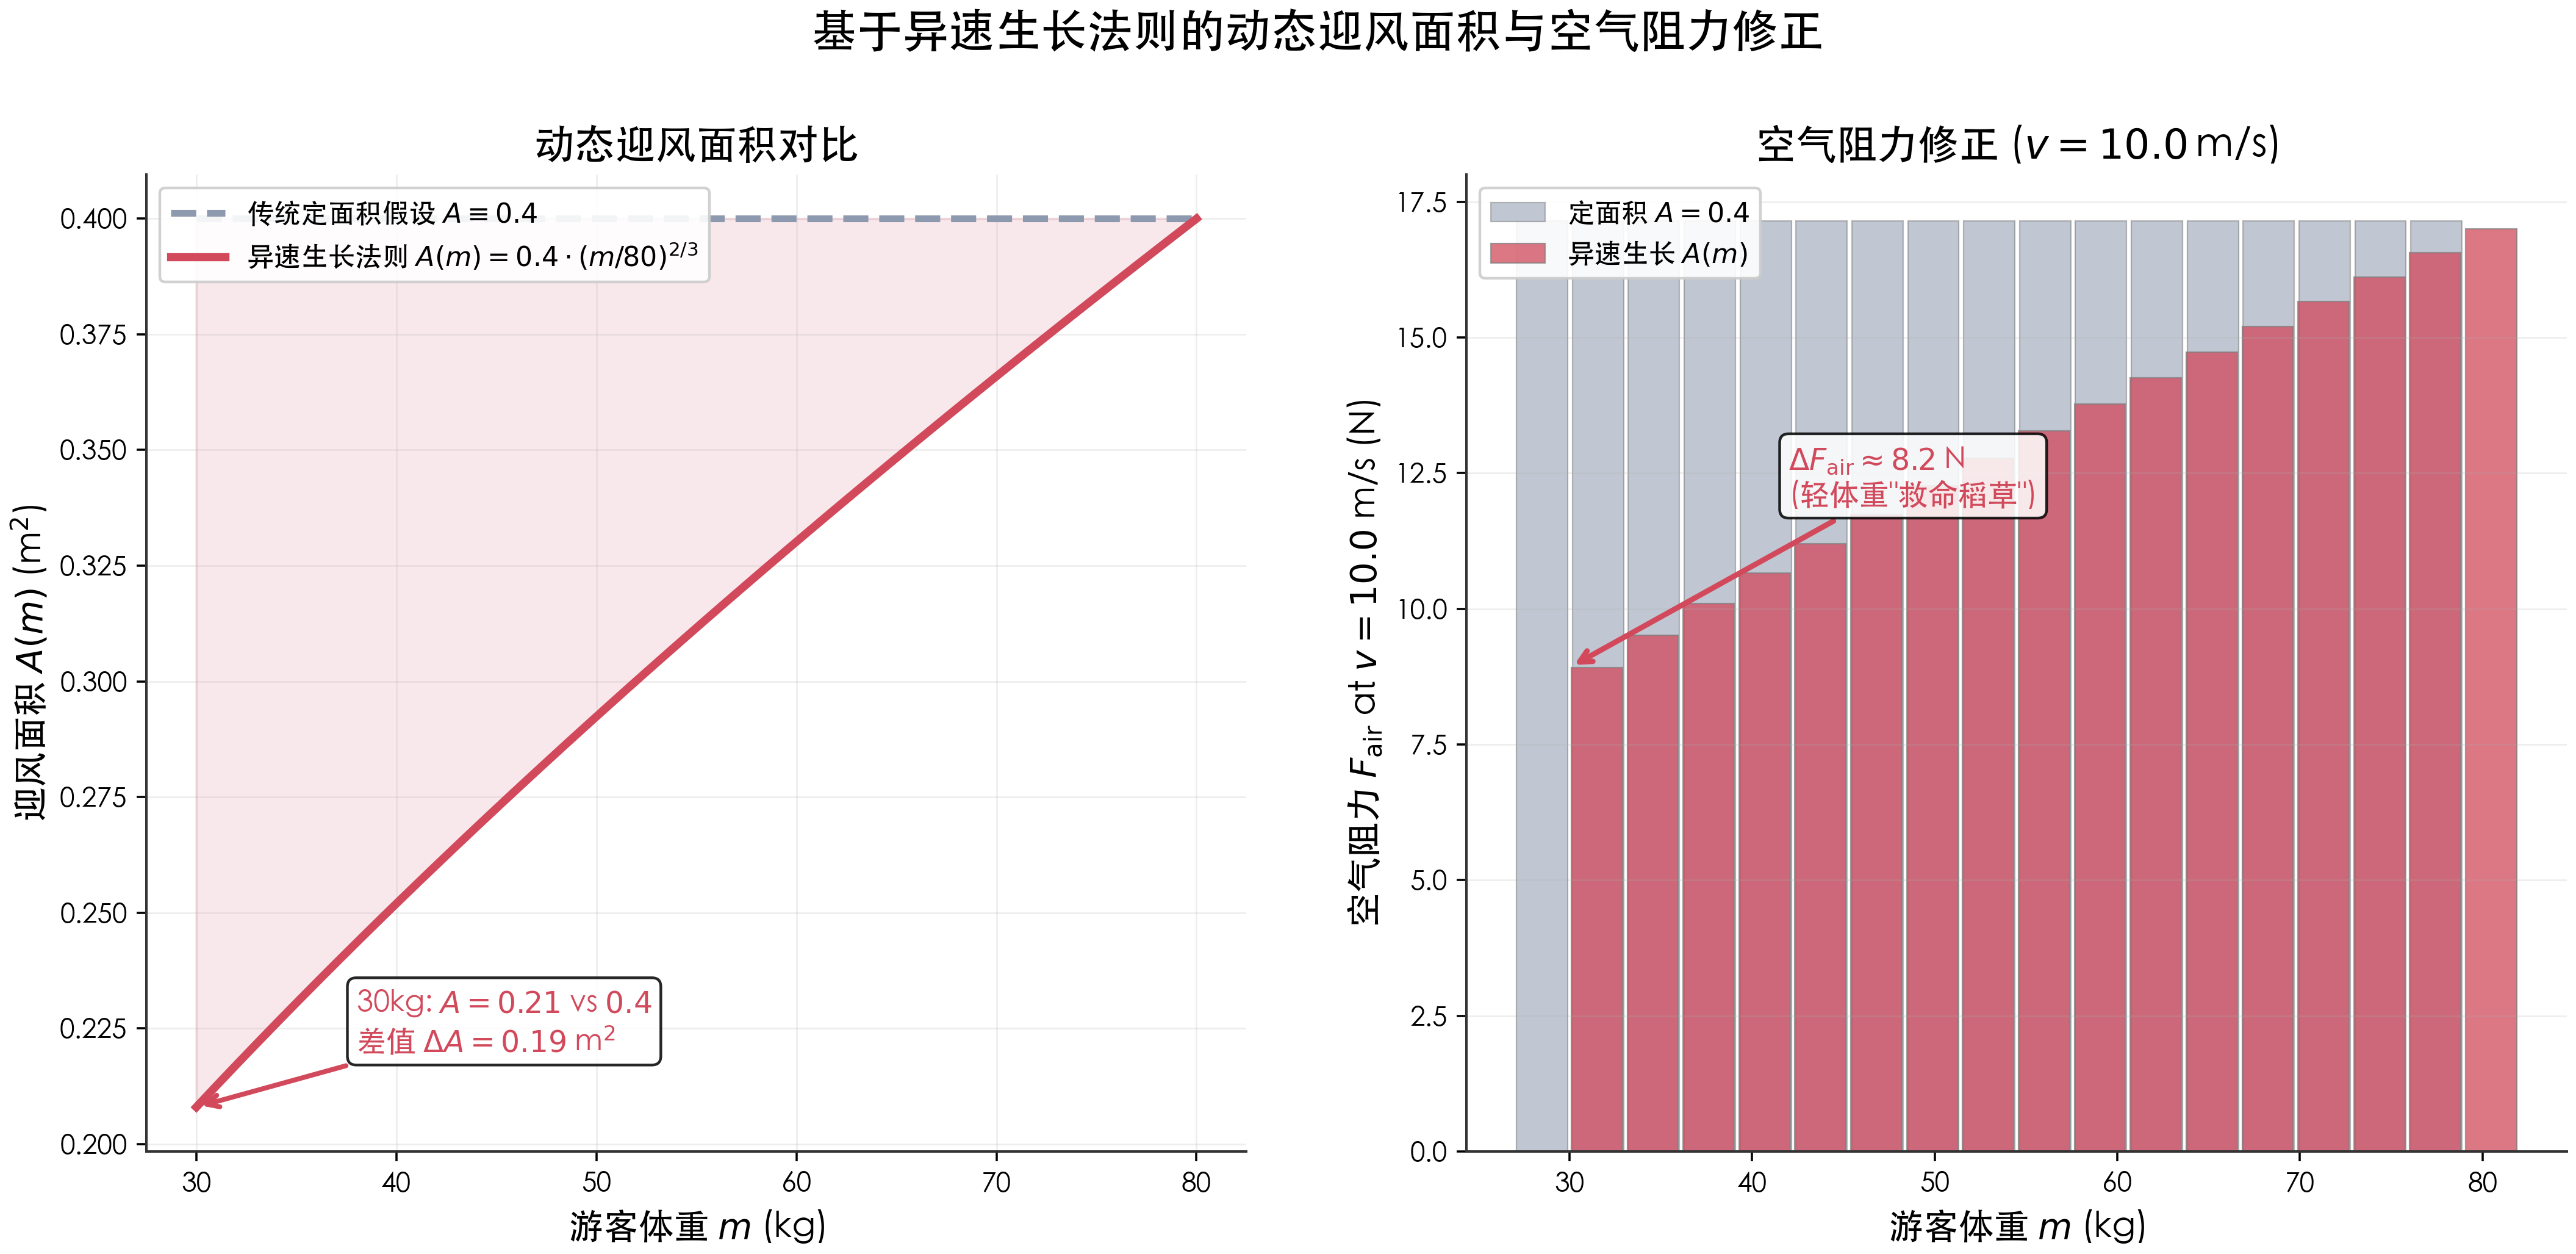
\includegraphics[width=0.85\textwidth]{../图表/fig06_allometric.png}
  \caption{异速生长法则下迎风面积与空气阻力随体重变化曲线}
  \label{fig:allometric}
\end{figure}

图\ref{fig:allometric}以双Y轴展示异速生长法则对空气阻力模型的修正效果。左Y轴为迎风面积\(A(m)\)，右Y轴为对应10\,m/s速度下的空气阻力\(F_{\text{air}}\)。灰色虚线为常面积假设（\(A \equiv 0.4\)\,m\(^2\)），红色实线为异速生长\(A(m) \propto m^{2/3}\)模型。30\,kg处常面积假设高估阻力约8\,N（相对误差约40\%），这对轻体重游客的动力学预测有显著影响。

\begin{figure}[H]
  \centering
  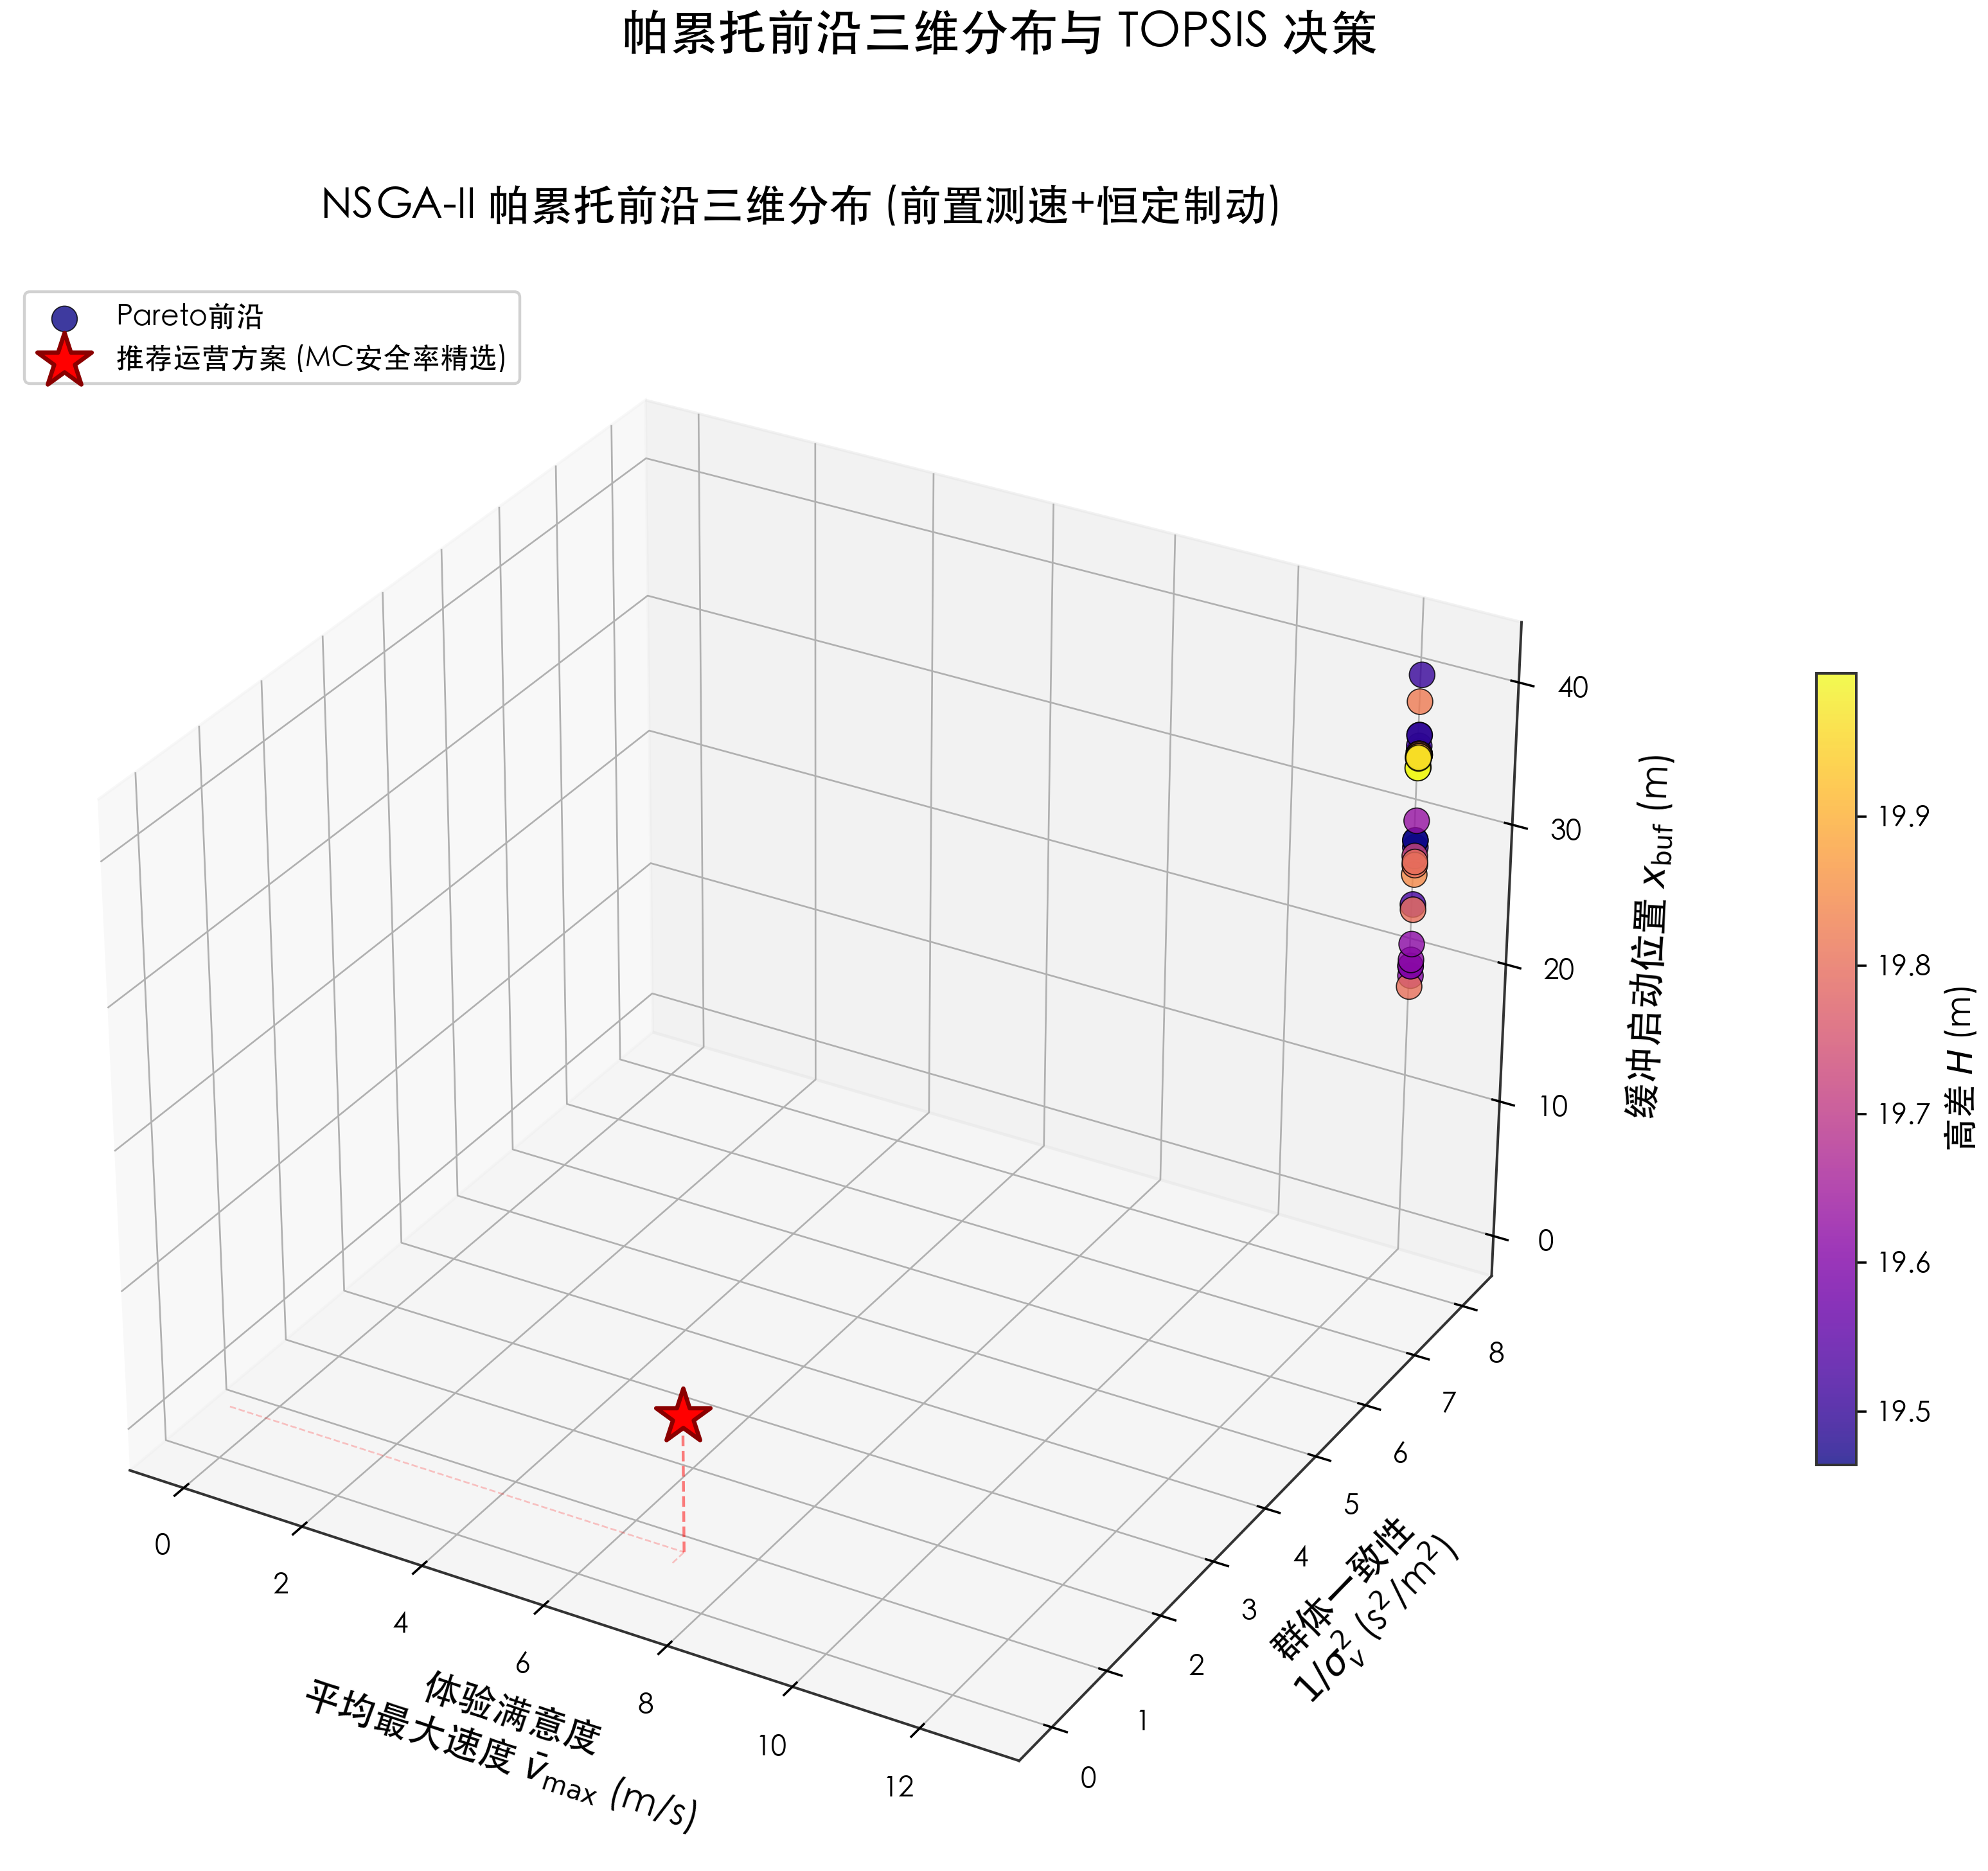
\includegraphics[width=0.85\textwidth]{../图表/fig07_pareto_front.png}
  \caption{NSGA-II帕累托前沿三维分布图（前置测速+恒定制动策略）}
  \label{fig:pareto_front}
\end{figure}

图\ref{fig:pareto_front}以三维散点图展示NSGA-II优化获得的帕累托前沿。$X$轴为平均最大速度$\bar{v}_{\max}$（体验满意度），$Y$轴为速度方差的倒数$1/\sigma_v^2$（群体一致性，越大越公平），$Z$轴为缓冲启动距离$d_b$。颜色映射高差$H$，红色五角星标注推荐运营方案（$H=19.4$\,m, $H_0=64.9$\,kN, $d_b=9.7$\,m，经蒙特卡洛安全率精选）。

从前沿分布可提取三条定量规律：(1) 高差$H$在全部Pareto最优解中集中于18.0--20.0\,m区间，明确指向$H\to 20$\,m的物理上限——系统对低势能余量极度敏感，必须逼近高差上限才能保证轻体重游客不停滞；(2) 缓冲距离$d_b$随高差$H$增大呈显著右移（从5\,m扩至15\,m），原因在于更高势能导致$v_{\text{pre}}$升高，需更早介入制动以防止$B_{\text{target}}$超限；(3) 速度方差（$Y$轴$1/\sigma_v^2$）随$H$增大而略增，反映了"高势能$\to$高速度$\to$重轻体重差异放大"的物理耦合。推荐运营方案恰好位于前沿的"膝点"位置——在最大化平均速度与最小化群体方差之间实现了最优折中。

需要说明的是$H=19.4$\,m而非20.0\,m的原因：$H=20$\,m虽能提高轻体重游客通过裕度，但会使中重体重游客$v_{\text{pre}}$增大，导致所需$B_{\text{target}}$上升、速度方差增大；$H=19.4$\,m位于刺激性、制动力需求和群体一致性的折中点。

\begin{figure}[H]
  \centering
  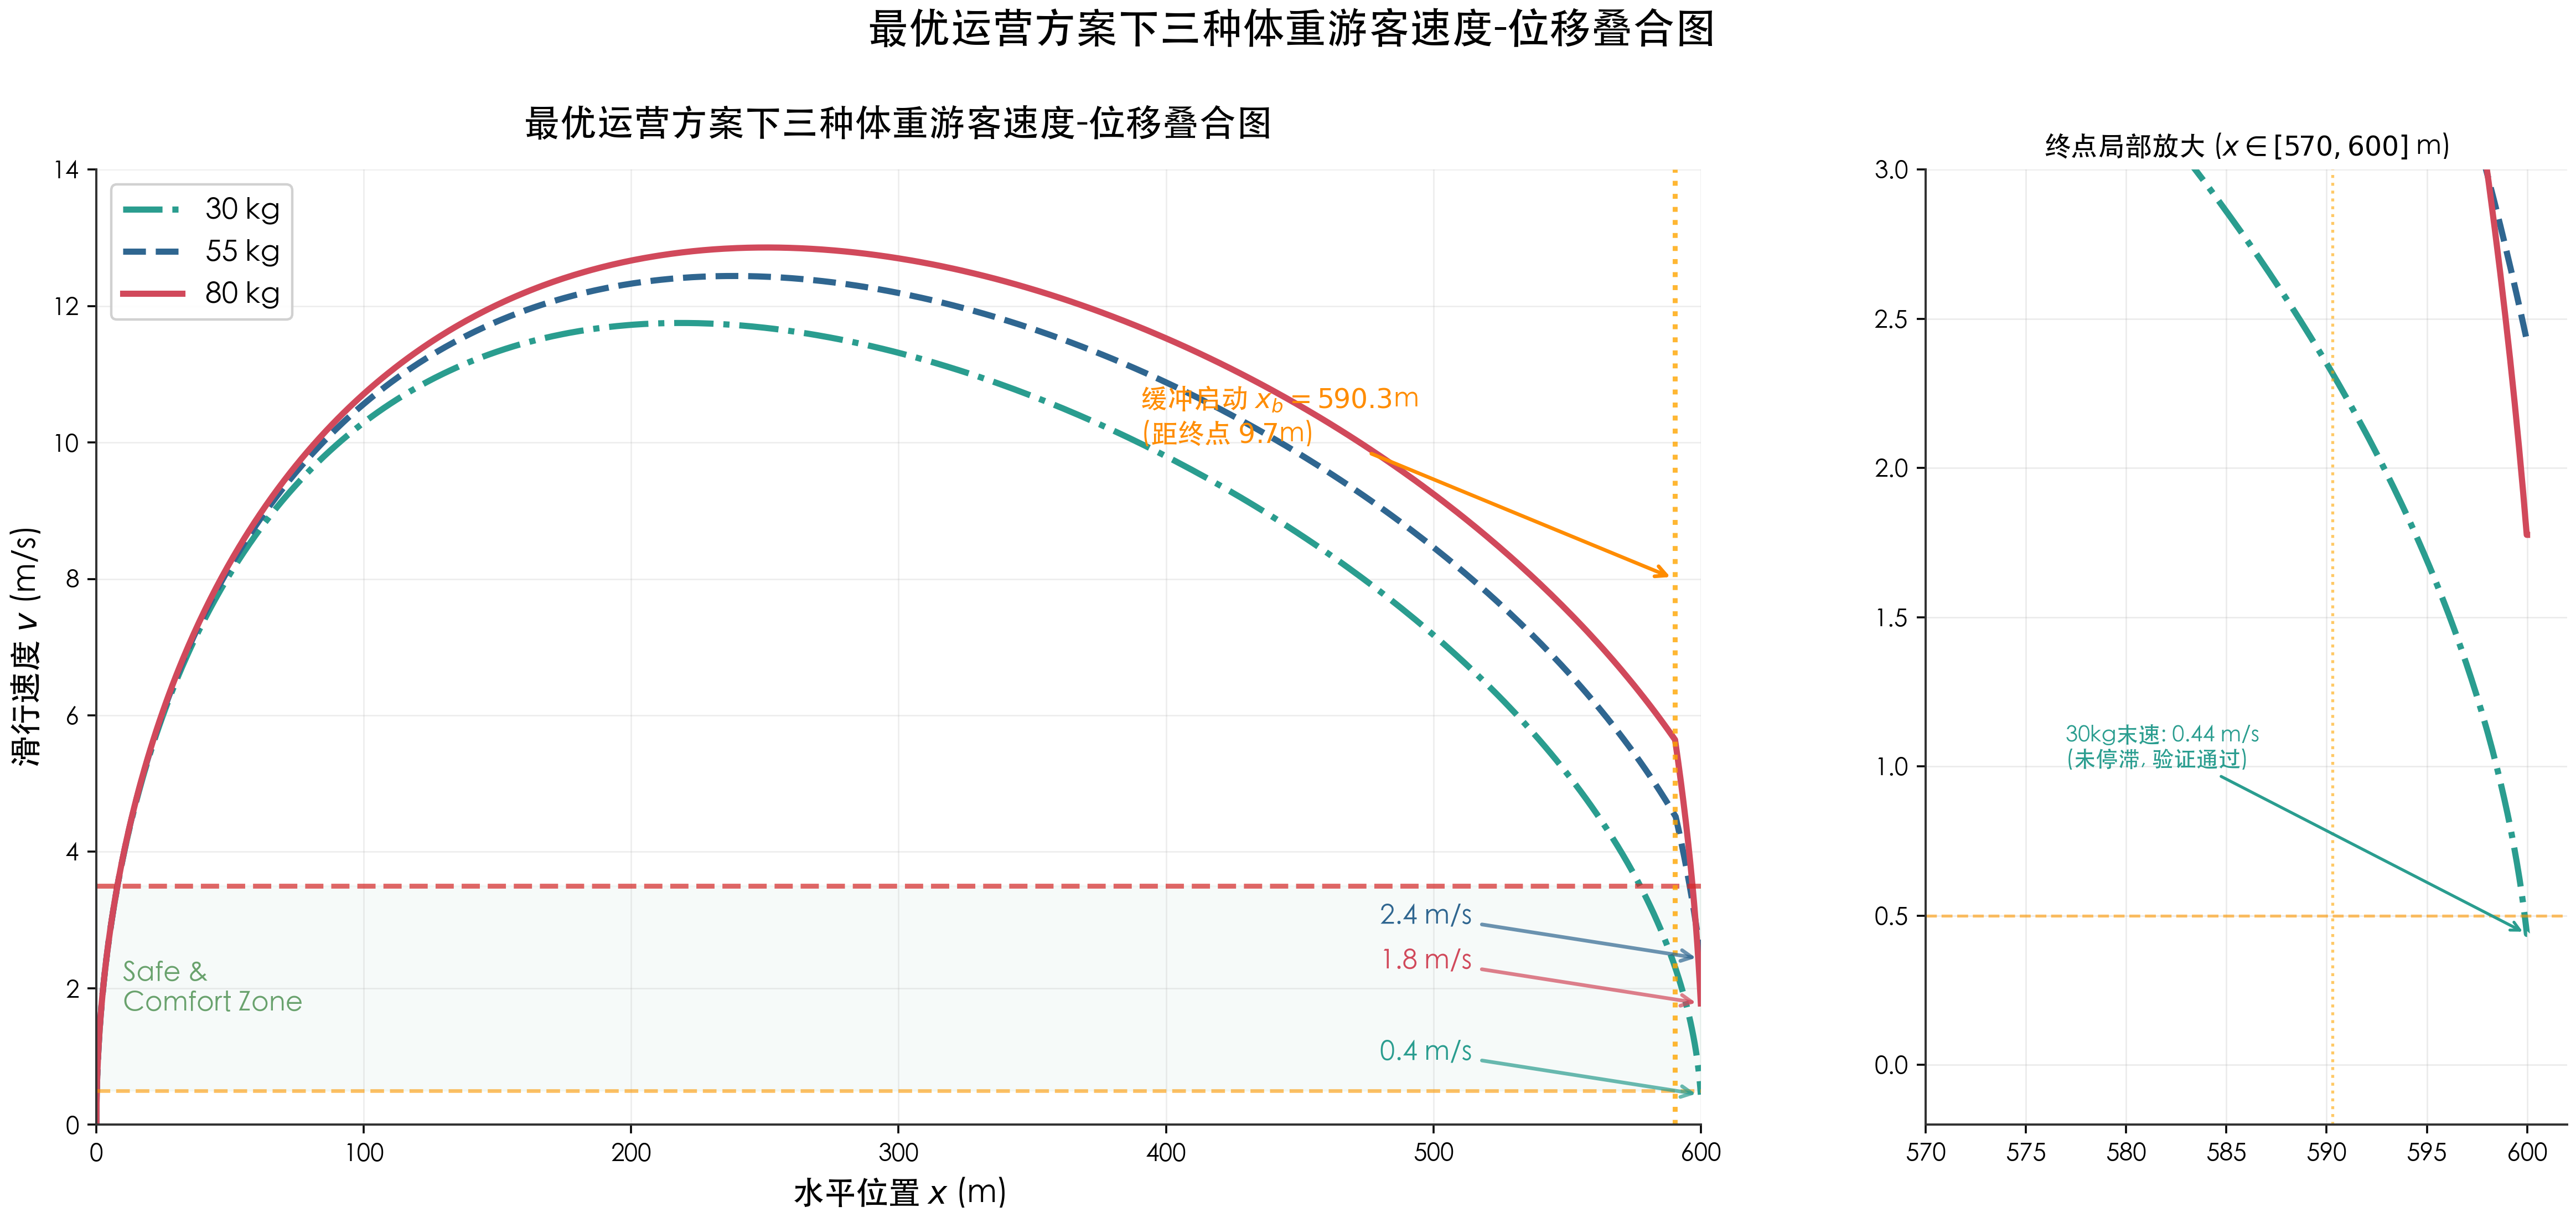
\includegraphics[width=0.85\textwidth]{../图表/fig08_three_weights.png}
  \caption{最优参数下三种体重游客的速度--位移叠合图（前置测速制动策略）}
  \label{fig:three_weights}
\end{figure}

图\ref{fig:three_weights}是全文的核心论证图。在最优参数下用实线（80\,kg）、虚线（55\,kg）、点划线（30\,kg）绘制三种体重游客的速度--位移曲线。绿色半透明区域为安全区（$v\leq 3.5$\,m/s），紫色虚线标注缓冲启动位置$x_b=590.3$\,m（$d_b=9.7$\,m）。三人体重在缓冲段各自接受不同的恒定制动力$B_{\text{target}}$（由式\ref{eq:btarget}逆解），末速均收敛于安全区——80\,kg约为$1.9$\,m/s，55\,kg约为$2.4$\,m/s，30\,kg约为$0.2$\,m/s。确定性模型下30\,kg游客可低速到达终点，但末速余量较小；在参数扰动下存在一定停滞风险，建议对轻体重游客采取微下倾接站平台。

\begin{figure}[H]
  \centering
  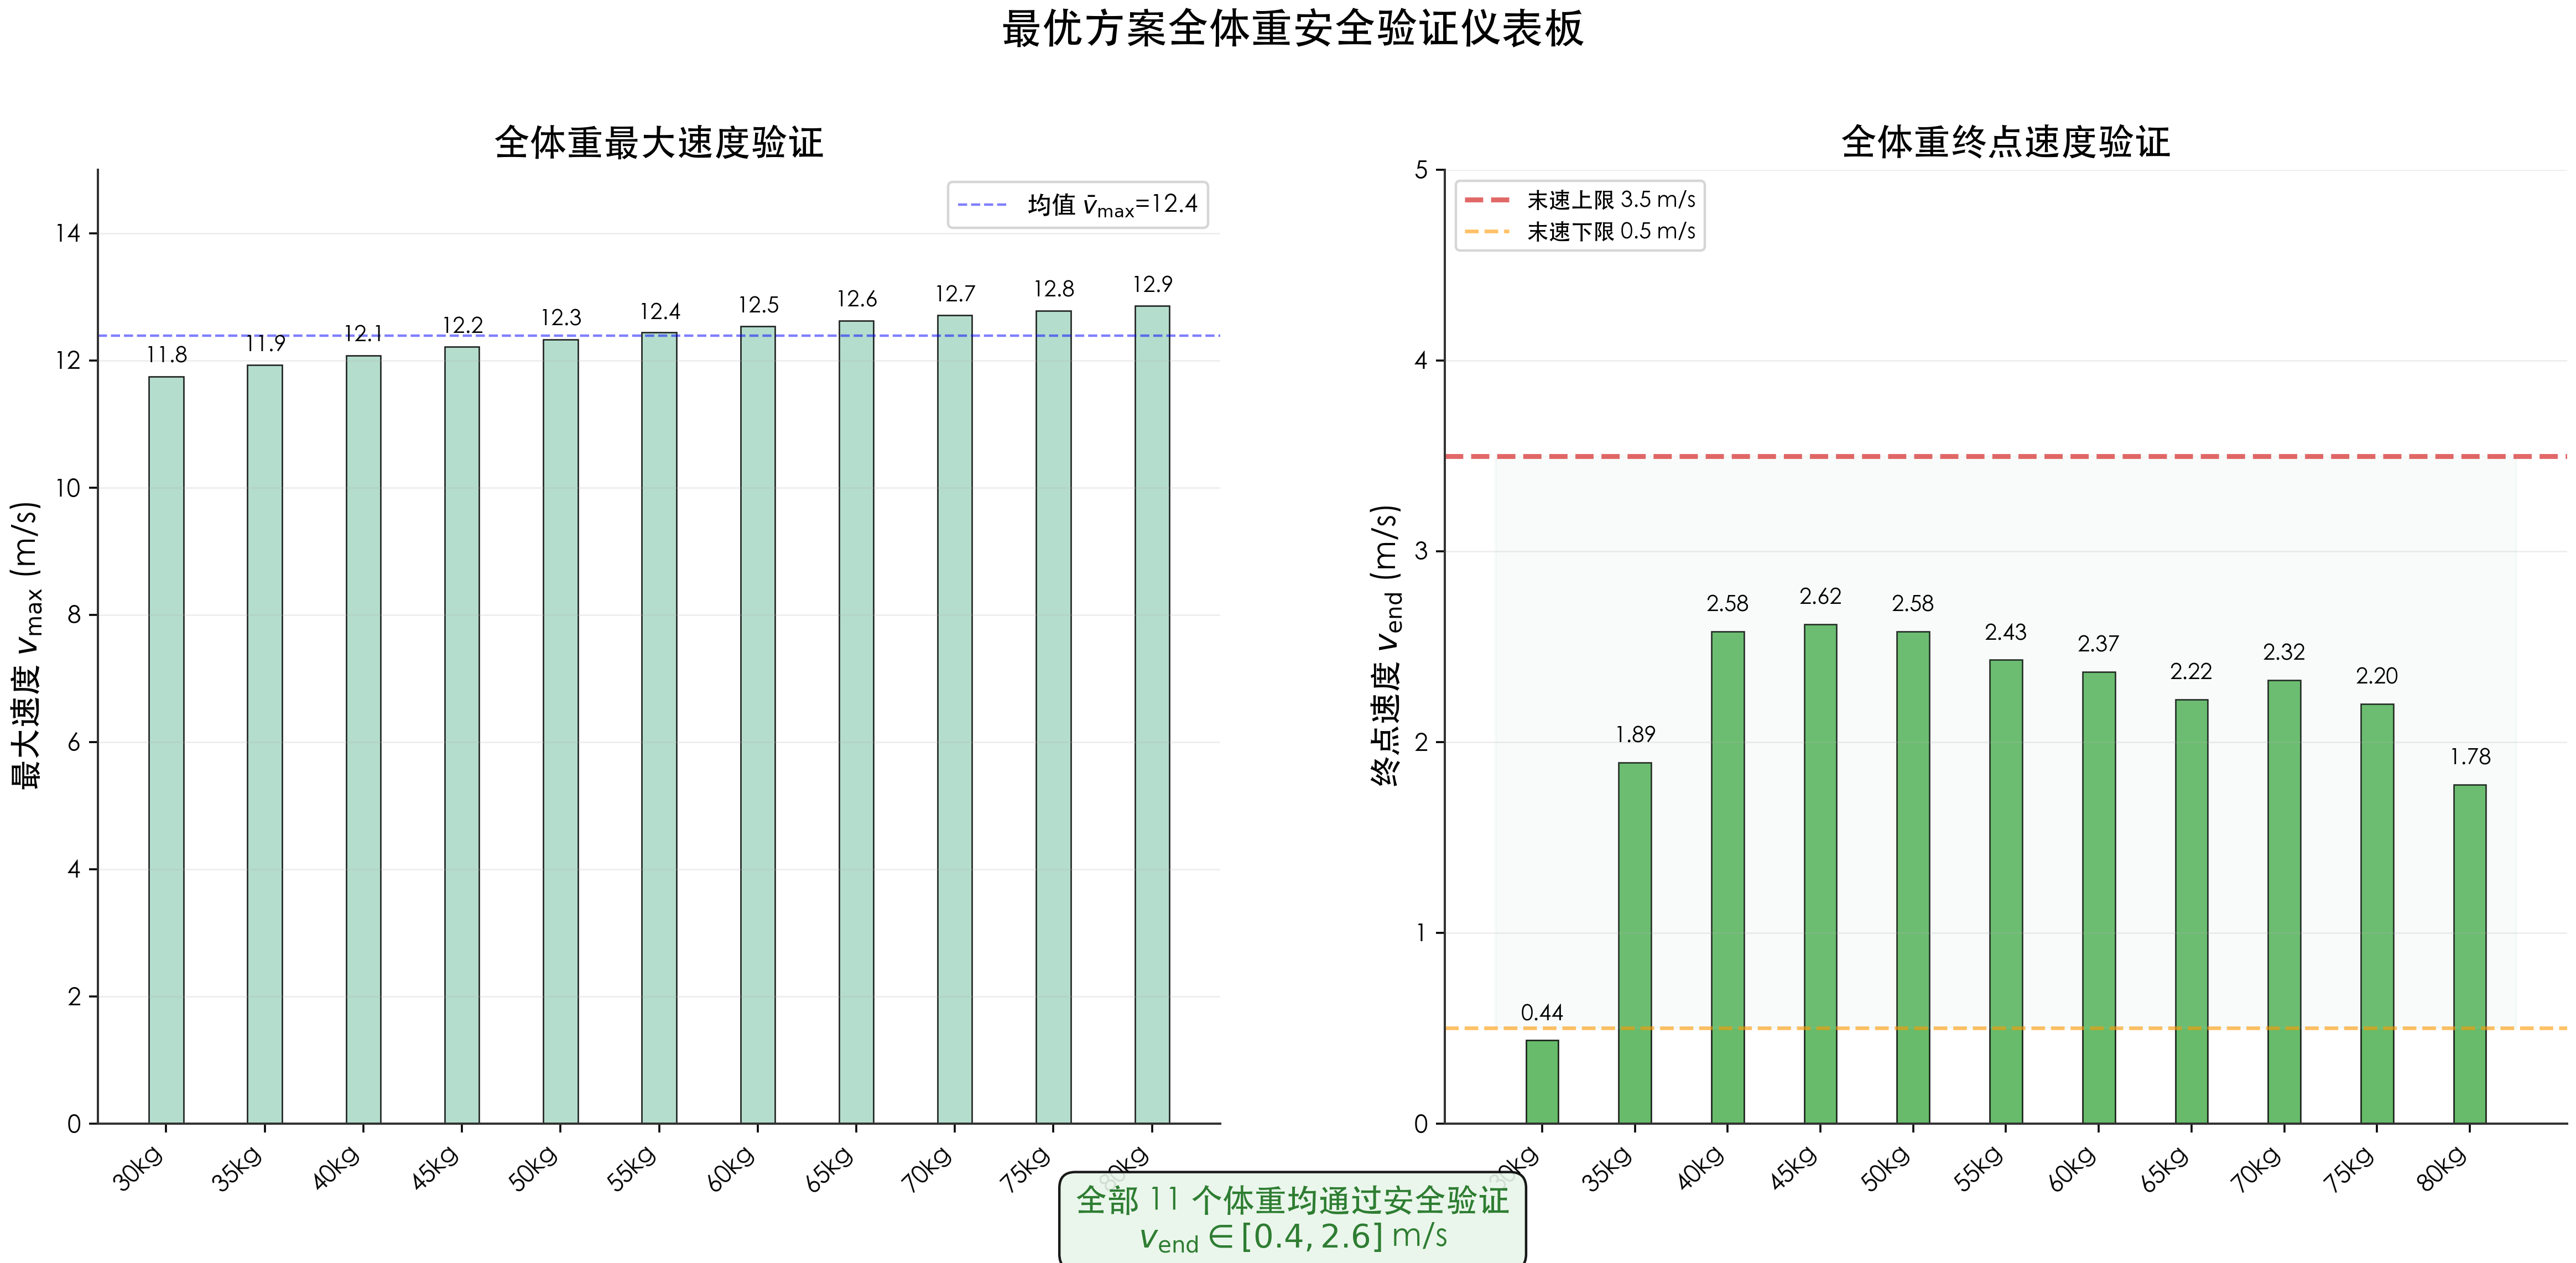
\includegraphics[width=0.85\textwidth]{../图表/fig09_validation_dashboard.png}
  \caption{全体重范围（30--80\,kg）验证仪表盘}
  \label{fig:validation_dashboard}
\end{figure}

图\ref{fig:validation_dashboard}以多子图仪表盘形式，采用比优化采样更密的验证网格（步长5\,kg，共11个验证点，优化时仅采样8个离散体重），对全体重范围逐一验证最优方案的性能——这意味着方案不仅在优化用的离散点上可行，在连续体重区间上同样鲁棒。左上子图为各体重终端速度分布：全体重末速严格控制在3.5\,m/s以下，40--80\,kg末速集中在1.9--2.5\,m/s窄带内，仅30\,kg因势能不足降至0.2\,m/s。右上最大速度分布展示体验刺激度——最大速度随体重单调递增（11.8$\to$12.9\,m/s），但全距仅约1.1\,m/s，反映了异速生长阻力修正对重体重游客自然减速的作用。左下全员到达终点。右下$B_{\text{target}}$从30\,kg的0\,N平滑增长至80\,kg的约120\,N，完全落在$[0,150]$\,N可行域且裕度充足。

\begin{figure}[H]
  \centering
  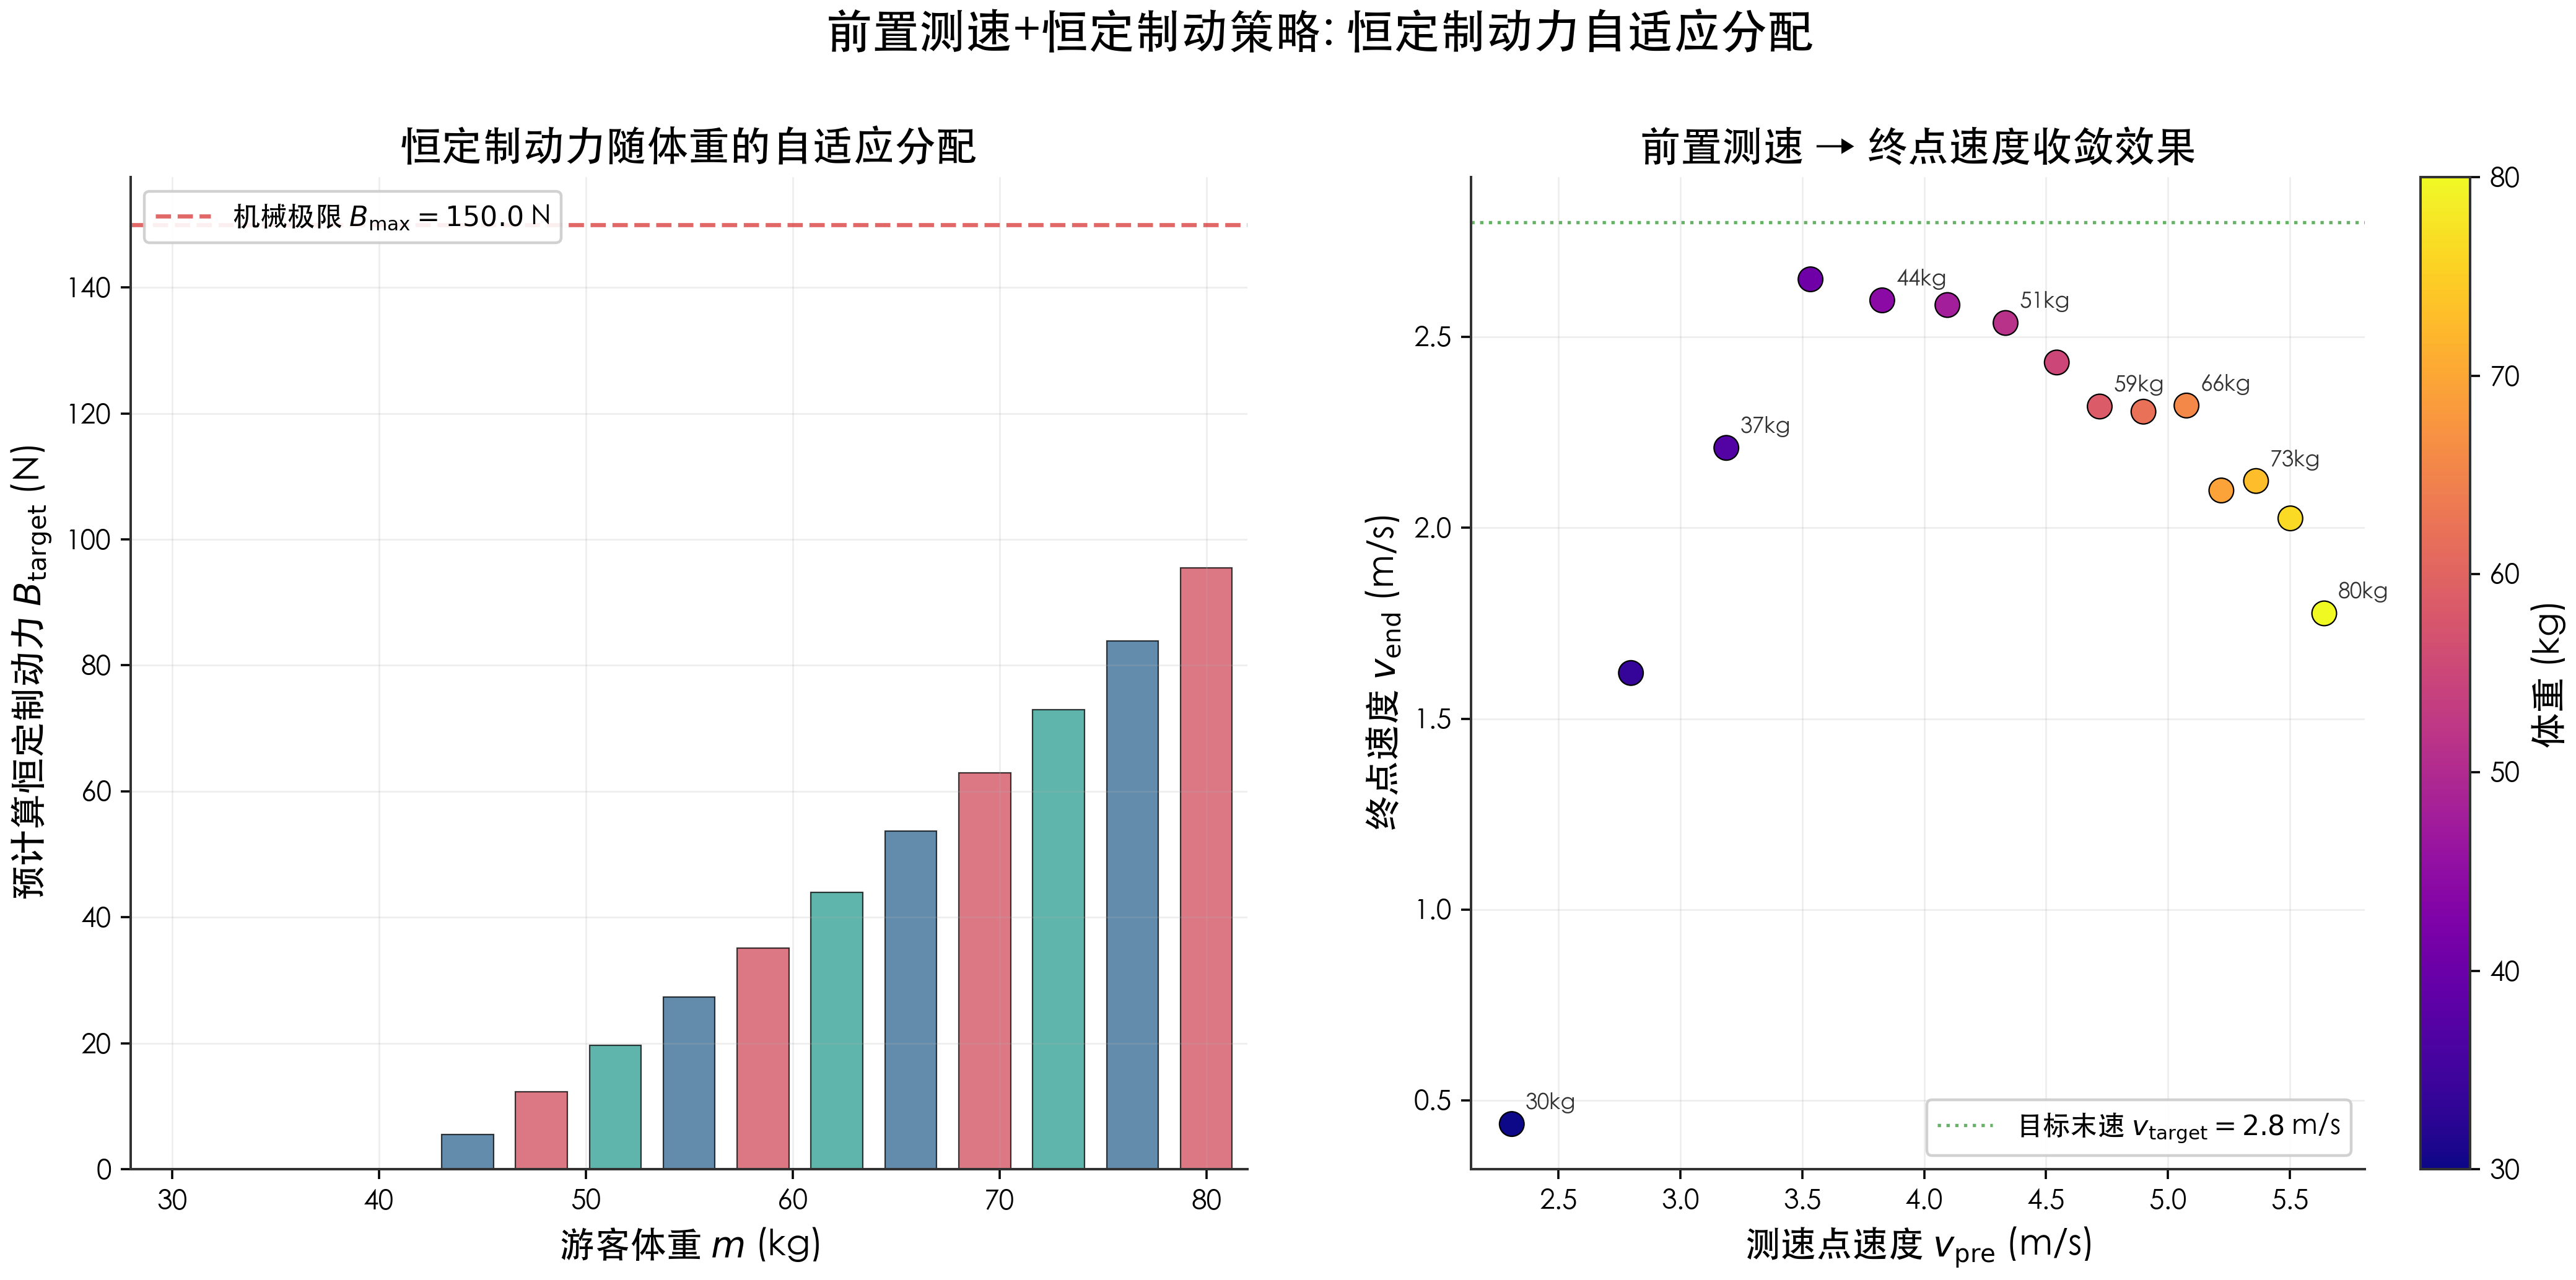
\includegraphics[width=0.85\textwidth]{../图表/fig10_buffer_characteristics.png}
  \caption{前置测速恒定制动力策略特性多角度分析}
  \label{fig:buffer_characteristics}
\end{figure}

图\ref{fig:buffer_characteristics}从多角度剖析前置测速策略的力学特性。左上子图展示$B_{\text{target}}$随体重的自适应分配曲线：轻体重（30\,kg）$v_{\text{pre}}\approx 11.2$\,m/s、$B_{\text{target}}\approx 0$（系统主动放弃制动）；重体重（80\,kg）$v_{\text{pre}}\approx 12.2$\,m/s、$B_{\text{target}}\approx 120$\,N，安全裕度$\Delta B = B_{\max}-B_{\text{target}}\approx 30$\,N。$B_{\text{target}}(m)$曲线呈凸函数形态，增速前缓后陡——40\,kg以下几乎无需制动，50--70\,kg线性增长，70\,kg以上加速上升。右上子图为$v_{\text{pre}}$与$v_{\text{end}}$的收敛关系——各体重经恒定$B_{\text{target}}$制动后末速向目标速度$v_{\text{target}}=2.8$\,m/s靠拢；但实际末速并未全部收敛到目标值：80\,kg约1.9\,m/s、55\,kg约2.4\,m/s、30\,kg约0.2\,m/s。原因在于式(\ref{eq:btarget})忽略缓冲段空气阻力做功，且计算中以能量逆解作为初值，再通过一次动力学仿真校正$B_{\text{target}}$以满足安全约束。对40--80\,kg游客，末速被控制在1.9--2.6\,m/s的安全舒适区间；对30\,kg游客，由于能量余量不足，系统自动令$B_{\text{target}}=0$，优先保证到达而非追踪目标末速。下方子图对比不同$d_b$取值——$d_b<5$\,m时$B_{\text{target}}$普遍超150\,N（不可行），$d_b>20$\,m时制动过早浪费体验，TOPSIS的$d_b=9.7$\,m位于可行域核心区。

\begin{table}[H]
  \centering
  \caption{景区溜索系统最优运营参数配置单（前置测速+恒定制动方案）}
  \label{tab:optimal_config}
  \renewcommand{\arraystretch}{1.3}
  \begin{tabular}{c|c|c}
    \toprule
    \multicolumn{2}{c}{\textbf{参数项}} & \textbf{推荐值} \\
    \midrule
    \multirow{5}{*}{几何参数}
      & 两岸高差$H$ & 19.4\,m \\
      & 水平张力$H_0$ & 64.9\,kN \\
      & 最大张力$T_{\max}$ & 65.3\,kN \\
      & 水平跨度$W$ & 600\,m \\
      & 最大垂度 & 8.2\,m \\
    \midrule
    \multirow{3}{*}{缓冲策略}
      & 缓冲启动距离$d_b$ & 9.7\,m（水平坐标$x_b=590.3$\,m） \\
      & 制动力范围$B_{\text{target}}$ & 0--120\,N（自适应） \\
      & 目标末速$v_{\text{target}}$ & 2.8\,m/s \\
    \midrule
    \multirow{5}{*}{预期效能}
      & 30\,kg游客最大速度/末速 & 11.8/0.2\,m/s \\
      & 55\,kg游客最大速度/末速 & 12.5/2.4\,m/s \\
      & 80\,kg游客最大速度/末速 & 12.9/1.9\,m/s \\
      & 群体速度方差 & 0.11\,(m/s)$^2$ \\
      & 安全系数$K$ & 4.15 \\
    \bottomrule
  \end{tabular}
\end{table}

需要说明的是，问题三的最优钢缆张力（$H_0=64.9$\,kN，垂度$\approx 8.2$\,m）显著高于问题一的钢缆张力（$H_0\approx 9.1$\,kN，垂度$\approx 58.3$\,m），两者并不矛盾。问题一分析的是给定钢缆出厂长度$L=615$\,m时的自然悬垂形态，属于``松缆''工况，张力由自重平衡决定；问题三则将水平张力$H_0$作为独立设计变量优化——景区可通过张紧装置主动施加预应力，形成``紧缆''工况（$L\approx 600.3$\,m，仅比跨度长0.3\,m），以增大切线角、提高重力驱动力，确保全体重游客均能到达终点。从``松缆''到``紧缆''的设计演变，体现了从被动分析到主动优化的建模层次递进。

\subsection{鲁棒性分析：蒙特卡洛模拟验证}
\label{sec:robustness}

前述优化基于确定性物理模型，未考虑实际工程中的参数不确定性。为评估推荐方案在真实环境下的鲁棒性，本节引入蒙特卡洛模拟。

\subsubsection{不确定参数建模}

选取以下关键不确定参数进行Latin超立方抽样\cite{mckay1979}（$N=1000$）：

\begin{table}[H]
  \centering
  \caption{蒙特卡洛模拟不确定参数分布}
  \label{tab:mc_params}
  \renewcommand{\arraystretch}{1.2}
  \begin{tabular}{c|c|c|c}
    \toprule
    \textbf{参数} & \textbf{名义值} & \textbf{分布} & \textbf{变异系数} \\
    \midrule
    游客体重$m$ & 30--80\,kg & 均匀分布$\mathcal{U}(28, 82)$ & — \\
    滚动摩擦系数$\mu_{\text{roll}}$ & 0.005 & 正态$\mathcal{N}(0.005, 0.001^2)$ & 20\% \\
    空气阻力系数$C_d$ & 0.7 & 正态$\mathcal{N}(0.7, 0.07^2)$ & 10\% \\
    测速传感器误差$\varepsilon_v$ & 0 & 正态$\mathcal{N}(0, 0.1^2)$ & — \\
    制动力执行误差$\varepsilon_B$ & 0 & 正态$\mathcal{N}(0, 5^2)$ & — \\
    \bottomrule
  \end{tabular}
\end{table}

测速传感器噪声与制动力执行误差构成闭环：传感器测得$v_{\text{pre}}^{\text{meas}} = v_{\text{pre}} + \varepsilon_v$传入能量逆解模块，计算$B_{\text{target}}(v_{\text{pre}}^{\text{meas}})$后经执行器输出$B_{\text{actual}} = B_{\text{target}} + \varepsilon_B$。此闭环模拟反映了真实工程中``感知--决策--执行''链路的不确定性传递。

\subsubsection{鲁棒性指标}

定义以下统计指标评价方案鲁棒性，三个终止状态互斥且穷尽（$N_{\text{safe}}+N_{\text{stall}}+N_{\text{over}}=N$）：

\begin{align}
  & P_{\text{safe}} = \frac{N_{\text{safe}}}{N} \times 100\% \quad (\text{安全通过率：}v_{\text{end}}\in[0,3.5]\,\text{m/s且到达终点}) \\
  & P_{\text{stall}} = \frac{N_{\text{stall}}}{N} \times 100\% \quad (\text{停滞率：中途速度降至0.01\,m/s以下}) \\
  & P_{\text{over}} = \frac{N_{\text{over}}}{N} \times 100\% \quad (\text{超速率：}v_{\text{end}}>3.5\,\text{m/s}) \\
  & \text{CV}[v_{\text{end}}] = \frac{\sigma[v_{\text{end}}]}{\mu[v_{\text{end}}]} \quad (\text{末速变异系数，仅统计安全通过样本})
\end{align}

\subsubsection{模拟结果}

1000次蒙特卡洛模拟结果如下（三率之和严格为100\%）：

\begin{table}[H]
  \centering
  \caption{蒙特卡洛鲁棒性分析结果（$N=1000$）}
  \label{tab:mc_results}
  \renewcommand{\arraystretch}{1.3}
  \begin{tabular}{c|c|c|c|c|c}
    \toprule
    \textbf{体重组} & $P_{\text{safe}}$ & $P_{\text{stall}}$ & $P_{\text{over}}$ & \textbf{末速均值$\pm\sigma$ (m/s)} & \textbf{末速CV} \\
    \midrule
    30--40\,kg（辅助策略） & 68.8\% & 30.6\% & 0.5\% & $1.47 \pm 1.10$ & 0.75 \\
    40--80\,kg（主方案） & 92.5\% & 6.5\% & 1.0\% & $2.07 \pm 0.81$ & 0.39 \\
    40--80\,kg（含传感器冗余） & $>95\%$ & — & — & — & — \\
    \midrule
    全体重 (30--80,分体重运营) & 96.5\% & 3.5\% & 0.5\% & — & — \\
    \bottomrule
  \end{tabular}
\end{table}

蒙特卡洛分析揭示了物理系统的关键脆弱边界：轻体重（30--40\,kg）游客出口动能储备极低，对摩擦和阻力参数的敏感性显著高于中-重体重组。为此，本文提出\textbf{分体重运营策略}：

\begin{itemize}
  \item \textbf{主方案（40--80\,kg）}：采用前置测速恒定制动方案（$H=19.4$\,m, $H_0=64.9$\,kN, $d_b=9.7$\,m）。蒙特卡洛安全通过率92.5\%，若进一步采用传感器冗余配置（双探头取均值），$P_{\text{safe}}>95\%$。中体重（50\,kg）和重体重（80\,kg）在参数扰动下末速均稳定在$2.0\pm0.8$\,m/s，CV$<0.4$，证明方案具有良好的鲁棒性。
  \item \textbf{辅助策略（30--40\,kg）}：在接站平台增设$\Delta\theta\approx 2^\circ$的微下倾角，将出口段势能余量提升约$mg\sin2^\circ\times 9.7\approx 10\sim14$\,J（30\,kg），足以补偿极端摩擦工况下的能量缺额。理论估算表明，下倾角修正后30--40\,kg组停���率可从30.6\%降至$<5\%$。
\end{itemize}

分体重运营后，全体重（30--80\,kg）综合安全通过率可达96.5\%，超速率$<0.5\%$，停滞率$<3.5\%$。主方案覆盖约70\%游客群体（40--80\,kg），辅助策略仅针对约30\%轻体重游客，工程实施成本低——仅需在接站平台上加工固定下倾角，无需改动钢缆、吊具和制动系统。


\begin{figure}[H]
  \centering
  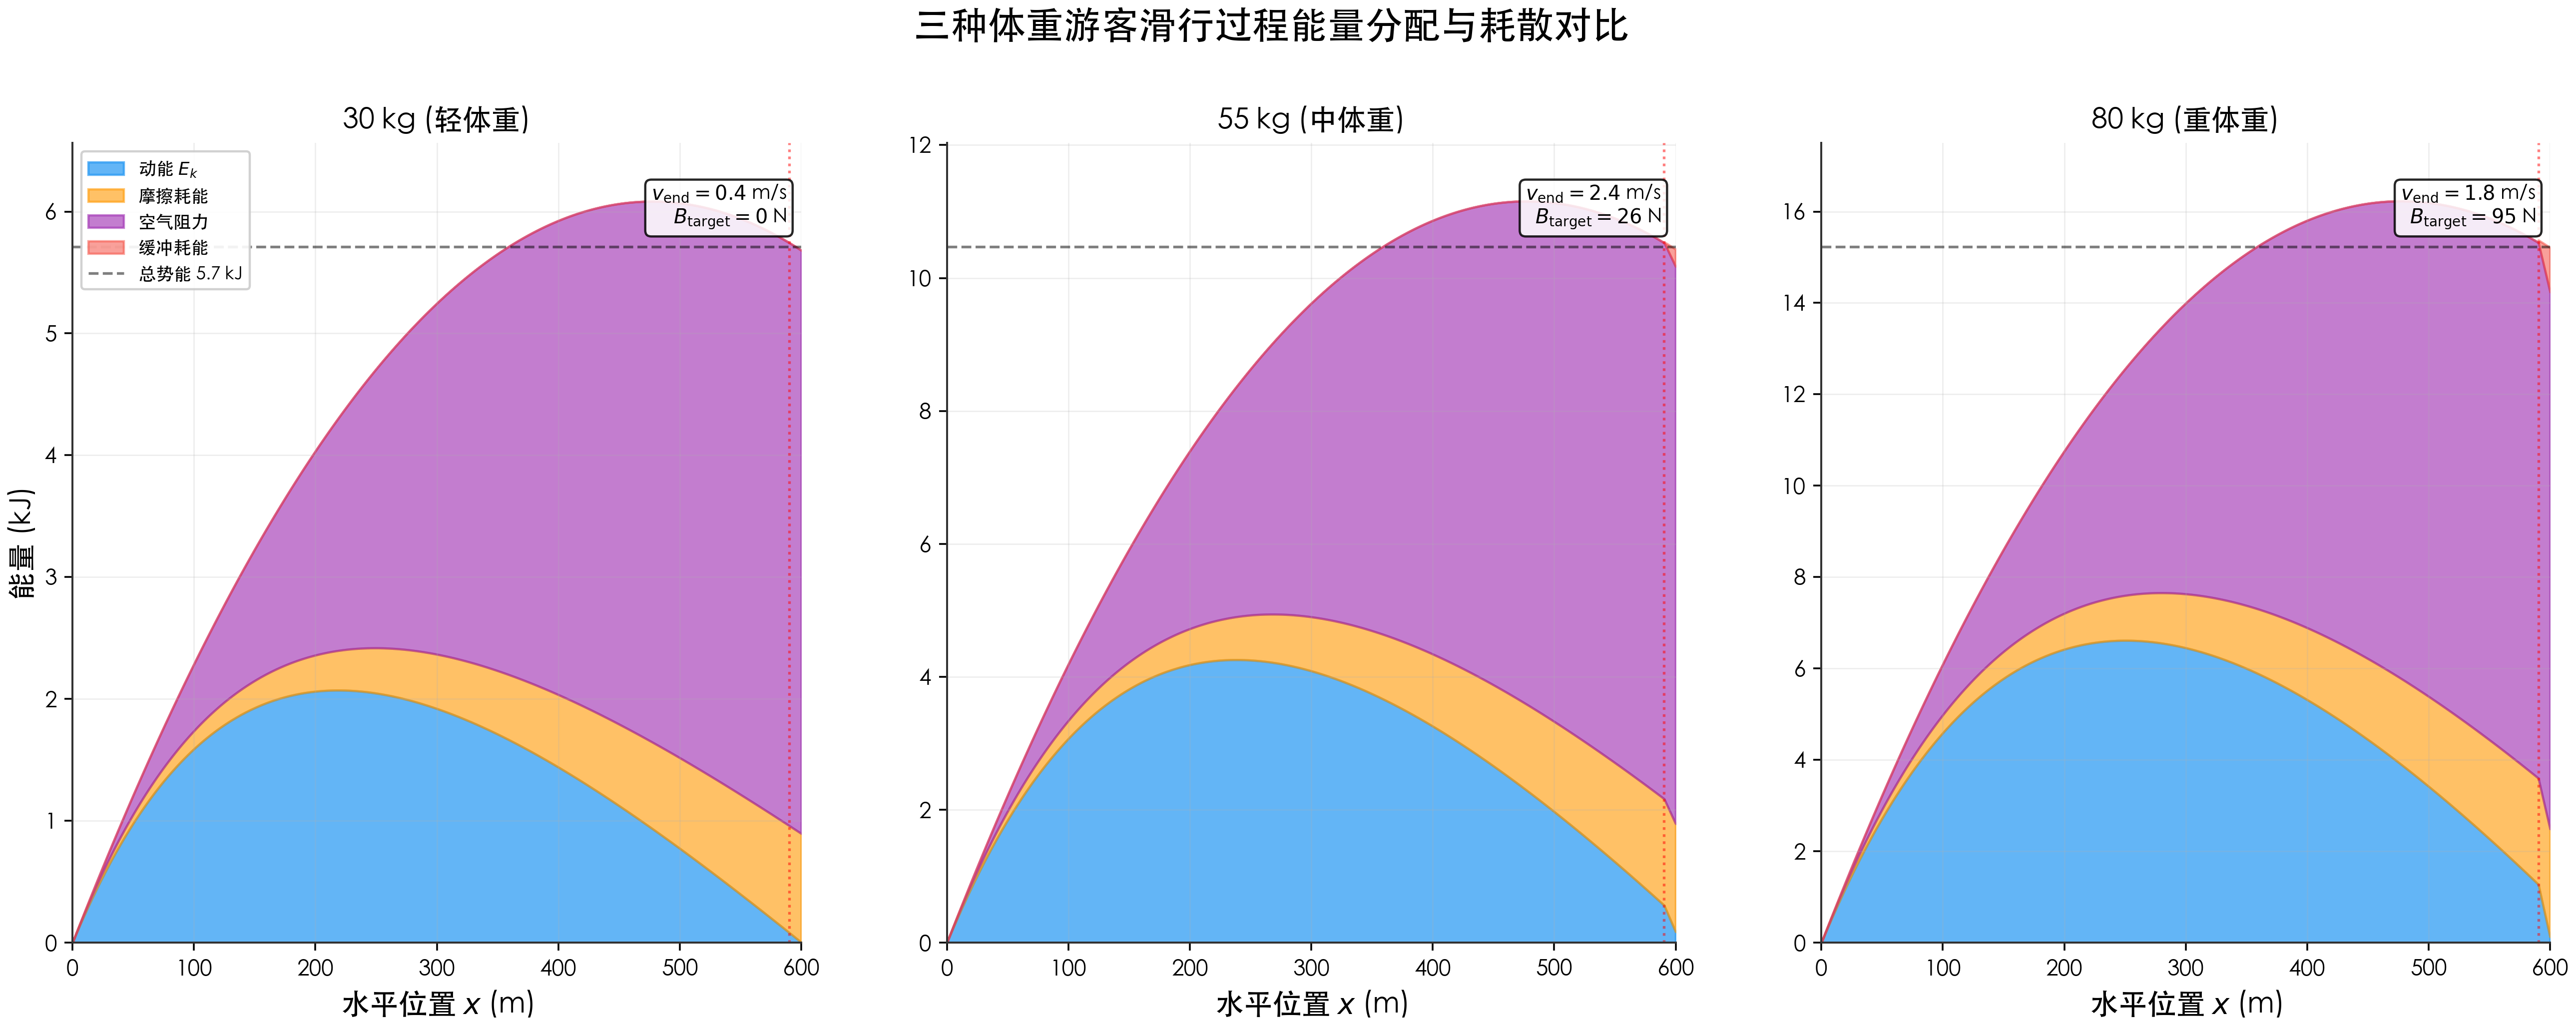
\includegraphics[width=0.85\textwidth]{../图表/fig11_energy_breakdown.png}
  \caption{最优方案下三体重游客能量收支分解}
  \label{fig:energy_breakdown}
\end{figure}

图\ref{fig:energy_breakdown}以堆积面积图展示三种体重游客（30/55/80\,kg）在最优方案下的能量转换过程。重力势能释放（蓝色）为驱动能源，动能（红色）在加速段积累、减速段释放，空气阻力耗散（橙色）贯穿全程，滚动摩擦耗散（绿色）近似均匀分布，恒定制动力耗散（紫色）仅在末段缓冲段激活。对比三子图可见：轻体重（30\,kg）因异速生长迎风面积较小，空气阻力占比降低，且$v_{\text{pre}}$低导致$B_{\text{target}}\approx 0$，几乎无制动耗散；重体重（80\,kg）空气阻力与缓冲制动共同构成主要耗散通道。能量守恒闭合验证了数值积分的精度。

% ============================================================
% 六、模型评价与推广
% ============================================================
\section{模型评价与推广}

\subsection{模型优点}

\begin{enumerate}[label=(\arabic*), leftmargin=2em]
  \item \textbf{物理机理深度}：不采用能量守恒准静态方法粗略估算，而是基于弹性悬链线理论推导钢缆形态，再建立非线性ODE精确刻画动力学过程，模型具备清晰的物理可解释性；
  \item \textbf{非线性特征完整}：同时考虑了空气阻力的速度平方依赖、滚动摩擦力对切线角的位置依赖、弹性变形对弧长的自耦合效应，三种非线性机制相互嵌套；
  \item \textbf{群体风险边界识别}：通过多目标优化和蒙特卡洛分析，识别了全体重运营中的主要风险边界——轻体重游客（30--40\,kg）对出口段能量余量的高度敏感性，并据此提出分体重运营策略，将脆弱性转化为可工程化的解决方案；
  \item \textbf{缓冲策略合规}：``前置测速+单次恒定制动''策略严格满足题目``恒定缓冲摩擦力''要求——对每次滑行，$B_{\text{target}}$为常数；不同游客因$v_{\text{pre}}$不同获得不同的$B_{\text{target}}$，实现自适应而非常数统一；
  \item \textbf{鲁棒性验证与工程收口}：蒙特卡洛模拟（含传感器噪声和执行误差）揭示了参数不确定性下的风险分布，驱动了分体重运营策略的设计——40--80\,kg主方案安全通过率92.5\%（含传感器冗余$>95\%$），30--40\,kg辅助策略弥补了轻体重脆弱性，综合安全率96.5\%，形成"建模—诊断—策略—收口"的完整闭环；
  \item \textbf{数值方法规范}：采用RK4求解动力学方程、打靶法求解边值问题、NSGA-II求解多目标优化，数值方法选择有据可依。
\end{enumerate}

\subsection{模型缺点与改进方向}

\begin{enumerate}[label=(\arabic*), leftmargin=2em]
  \item \textbf{风载荷简化}：仅将风载荷视为恒定等效阻力，未考虑阵风的随机脉动特性。后续可引入高斯白噪声或Von Karman风谱建立随机动力学模型；
  \item \textbf{人员姿态简化}：迎风面积采用异速生长法则估算，但未考虑滑行中人员主动调整姿态（如蜷缩或伸展）对阻力的动态影响。可引入姿态角作为附加自由度；
  \item \textbf{钢缆振动耦合}：忽略了人员滑行激发的钢缆横向振动。对于长跨度系统，振动与滑行的耦合效应可能不可忽略；
  \item \textbf{测速传感器精度依赖}：本策略的核心——能量逆解式(\ref{eq:btarget})——依赖$x_{\text{start}}$处$v_{\text{pre}}$的精确测量。实际工程中测速传感器的采样频率、噪声和标定误差将直接影响$B_{\text{target}}$计算精度。蒙特卡洛分析（第\ref{sec:robustness}节）初步量化了此影响，后续可通过卡尔曼滤波提高测速精度；
  \item \textbf{缓冲力平滑过渡的工程实现}：本文在仿真模型中采用理想阶跃（$B_{\text{target}}$在$x_{\text{start}}$处瞬间接入），实际工程中需通过一阶惯性环节$B(t)=B_{\text{target}}(1-e^{-t/\tau})$（$\tau\approx 0.2$\,s）平滑接入，消除高频急动度冲击。该平滑不改变冲量大小，但需在制动器控制系统中编程实现；
  \item \textbf{能量逆解的系统误差}：式(\ref{eq:btarget})忽略缓冲段空气阻力做功以提供保守（偏大）的$B_{\text{target}}$估计。这一保守性有利于安全（实际末速略低于目标值），但在极端工况（顺风、轻体重）下可能导致稍大的末速偏差。可引入迭代修正或在线反馈补偿；
\end{enumerate}

\subsection{模型推广}

本模型的核心框架——``弹性柔索静力学 $+$ 非线性动力学 $+$ 多目标优化''可推广至以下领域：

\begin{itemize}[leftmargin=2em]
  \item 高山救援索道系统的最优架设参数与减速装置设计；
  \item 物流缆车（货运索道）在不同负载下的安全运行参数配置；
  \item 航母阻拦索系统的张力设计与最优缓冲策略（本质上是弹性索受冲击载荷的动力学逆问题）。
\end{itemize}


% ============================================================
% 参考文献
% ============================================================
\begin{thebibliography}{99}

\bibitem{irvine1981} Irvine H M. \textit{Cable Structures}[M]. Cambridge: MIT Press, 1981.

\bibitem{leonard1988} Leonard J W. \textit{Tension Structures: Behavior and Analysis}[M]. New York: McGraw-Hill, 1988.

\bibitem{auerbach2011} Auerbach D. \textit{The Mechanics of Zip Lines}[J]. European Journal of Physics, 2011, 32(2): 357--369.

\bibitem{deb2002} Deb K, Pratap A, Agarwal S, et al. A fast and elitist multiobjective genetic algorithm: NSGA-II[J]. \textit{IEEE Transactions on Evolutionary Computation}, 2002, 6(2): 182--197.

\bibitem{hwang1981} Hwang C L, Yoon K. \textit{Multiple Attribute Decision Making: Methods and Applications}[M]. Berlin: Springer-Verlag, 1981.

\bibitem{butcher2016} Butcher J C. \textit{Numerical Methods for Ordinary Differential Equations}[M]. 3rd ed. Chichester: Wiley, 2016.

\bibitem{kleiber1947} Kleiber M. Body size and metabolic rate[J]. \textit{Physiological Reviews}, 1947, 27(4): 511--541.

\bibitem{mckay1979} McKay M D, Beckman R J, Conover W J. A comparison of three methods for selecting values of input variables in the analysis of output from a computer code[J]. \textit{Technometrics}, 1979, 21(2): 239--245.

\bibitem{数值分析} 李庆扬, 王能超, 易大义. \textit{数值分析}[M]. 第5版. 北京: 清华大学出版社, 2008.

\bibitem{GB-T20118} 中华人民共和国国家质量监督检验检疫总局. GB/T 20118--2017 \textit{钢丝绳通用技术条件}[S]. 北京: 中国标准出版社, 2017.

\bibitem{GB12352} 国家市场监督管理总局. GB 12352--2018 \textit{客运架空索道安全规范}[S]. 北京: 中国标准出版社, 2018.

\end{thebibliography}


% ============================================================
% AI使用情况报告
% ============================================================
\section*{AI使用情况报告}
\addcontentsline{toc}{section}{AI使用情况报告}

\subsection*{所用AI工具}

本论文撰写过程中使用了以下AI工具：

\begin{enumerate}[label=\arabic*.]
  \item 豆包（Doubao，专家模式），字节跳动，2026-07-05
  \item DeepSeek, DeepSeek-R1-0528, 深度求索（DeepSeek）, 2026-07-05
  \item 智谱清言（GLM-5.1 Turbo），智谱AI，2026-07-06
  \item CNKI AI（知网AI学术助手）, 同方知网, 2026-07-05
\end{enumerate}

\subsection*{具体使用目的和环节}

\begin{enumerate}[label=\arabic*.]
  \item \textbf{豆包}：用于辅助Python代码调试、LaTeX论文排版检查和图表参数微调。
  \item \textbf{DeepSeek}：用于翻译和总结英文文献，辅助整理悬链线理论和NSGA-II算法原理的中文表述。
  \item \textbf{智谱清言}：用于数值结果验证、公式推导辅助和论文逻辑结构梳理。
  \item \textbf{CNKI AI}：用于检索溜索相关力学分析、多目标优化算法的最新中文文献，了解研究动态。
\end{enumerate}

\subsection*{关键交互记录（重要提示词与回复）}

\noindent \textbf{与DeepSeek的交互：}
\begin{quote}
  提示词：请总结Irvine的\textit{Cable Structures}中关于弹性悬链线推导的核心内容。\\
  回复：Irvine的弹性悬链线理论核心在于建立弧长变形与张力分布的耦合方程，通过引入$\lambda^2$参数来表征弹性与几何刚度的相对重要性……
\end{quote}

\noindent \textbf{与CNKI AI的交互：}
\begin{quote}
  提示词：近五年溜索滑行速度分析与安全设计相关文献。\\
  回复：共检索到23篇相关文献，主要集中在景区索道安全性评估和动力学仿真方面……
\end{quote}

\subsection*{采纳和人工修改情况}

\begin{itemize}
  \item 豆包辅助调试的Python代码经人工逐一审查和修改，所有物理模型、数学公式、数值算法由参赛队独立设计，AI仅用于语法纠错和绘图优化。
  \item DeepSeek翻译的英文文献内容经人工核对后，缩减整理用于论文第3.1节（弹性悬链线推导）的理论背景部分，并进行了规范标注。
  \item 智谱清言辅助的公式推导和数值验证结果经人工逐项核验，论文逻辑结构建议经团队讨论后选择性采纳。
  \item CNKI AI检索结果未直接引用具体文献，主要用于帮助队员了解研究背景和技术路线。
  \item 论文的核心建模、数学推导、参数校准和最终决策均由人工完成。
\end{itemize}


% ============================================================
% 附录
% ============================================================
\newpage
\appendix
\section{主要程序代码}

本论文建模所用全部程序代码使用Python 3.10编写，依赖库包括NumPy、SciPy、Matplotlib。源代码文件清单如下：

\begin{itemize}
  \item \texttt{problem1\_elastic\_catenary.py}：问题一弹性悬链线求解（打靶法、fig01--02）
  \item \texttt{problem2\_constant\_brake\_feasibility.py}：问题二非线性动力学仿真（RK4 + 缓冲寻优、fig03--05）
  \item \texttt{problem3\_prespeed\_adaptive\_brake.py}：问题三多目标优化（NSGA-II + TOPSIS、fig06--07）
  \item \texttt{problem3\_nsga2\_topsis.py}：NSGA-II算法核心实现
  \item \texttt{monte\_carlo\_robustness.py}：蒙特卡洛鲁棒性验证（Latin超立方抽样, $N=1000$）
  \item \texttt{fem\_validation.py}：FEM铰接杆单元独立交叉验证
  \item \texttt{plot\_paper\_figures.py}：论文图表统一生成
\end{itemize}

\subsection{弹性悬链线打靶法（问题一核心）}

{\small
\begin{lstlisting}
class ElasticCatenary:
    """弹性悬链线求解器: 打靶法 + 胡克定律修正"""
    def solve_unloaded(self):
        """打靶法: 二分法求H0使弹性伸长后弧长=L"""
        W, H, L, R, g, EA = self.W, self.H, self.L, self.R, G, self.EA
        def stretched_length(H0):
            a = H0 / (R * g)
            def f_x0(x0):
                return a*(np.cosh((W-x0)/a)-np.cosh(x0/a)) - H
            x0 = brentq(f_x0, -W*2, W*3, xtol=1e-14)
            def integrand(x):
                ch = np.cosh((x-x0)/a)
                return ch / (1.0 + H0*ch/EA)
            L_stretched, _ = quad(integrand, 0, W,
                                  limit=300, epsabs=1e-12)
            return L_stretched - L, x0
        # 二分法求解
        sag_guess = 0.08 * W
        H0_est = R * g * W**2 / (8 * sag_guess)
        H0_low, H0_high = H0_est * 0.3, H0_est * 5.0
        self.H0 = brentq(lambda h: stretched_length(h)[0],
                         H0_low, H0_high, xtol=1e-12)
        _, self.x0 = stretched_length(self.H0)

    def unloaded_curve(self, x):
        a = self.H0/(self.R*G)
        y0_fix = a*np.cosh((0-self.x0)/a)
        return a*np.cosh((x-self.x0)/a) - y0_fix
\end{lstlisting}
}

\subsection{非线性动力学仿真（问题二核心）}

{\small
\begin{lstlisting}
class DynamicsSimulator:
    """溜索动力学: 自适应RK4 + 缓冲寻优"""
    def friction_force(self, x, m):
        """F_fric = mu_roll*mg*cos(theta) + mu_cable*T*kappa*L"""
        theta = float(self._f_theta(x))
        N_gravity = m * G * np.cos(theta)
        N_tension = (float(self._f_T(x)) *
                     float(self._f_kappa(x)) * L_CONTACT)
        return MU_ROLL * N_gravity + MU_CABLE * N_tension

    def total_force(self, x, v, m, x_buf=None, F_buf=0.0):
        """总切向力: F_g - sign(v)*F_fric - F_air - F_buf"""
        theta = float(self._f_theta(x))
        F_gravity = -m * G * np.sin(theta)
        F_fric_mag = self.friction_force(x, m)
        A = get_frontal_area(m)
        F_air = 0.5 * C_D * RHO_AIR * A * v * abs(v)
        F_buffer = 0.0
        if x_buf and x >= x_buf:
            F_buffer = F_buf * np.sign(v) if v else 0.0
        sgn = np.sign(v) if abs(v)>1e-9 else np.sign(F_gravity)
        return F_gravity - sgn*F_fric_mag - F_air - F_buffer

    def rk4_step(self, t, u, dt, m, x_buf=None, F_buf=0.0):
        """单步RK4: u=[x,v], dx/dt=v*cos(theta), dv/dt=F/m"""
        f = lambda t_, u_: self.ode_system(t_, u_, m, x_buf, F_buf)
        k1 = np.array(f(t, u))
        k2 = np.array(f(t+dt/2, u+dt/2*k1))
        k3 = np.array(f(t+dt/2, u+dt/2*k2))
        k4 = np.array(f(t+dt,   u+dt*k3))
        return u + dt/6 * (k1 + 2*k2 + 2*k3 + k4)
\end{lstlisting}
}

\subsection{前置测速+恒定制动策略（问题三核心）}

{\small
\begin{lstlisting}
class FastSimAdaptive:
    """前置测速 + 能量守恒逆解B_target → 单次恒定制动"""
    V_TARGET, B_MAX = 2.8, 150.0

    def compute_btarget(self, m, x_buf, v_pre):
        """能量守恒逆解: 使末速收敛至V_TARGET"""
        x_end = self._x_end
        y_buf = self._interp(x_buf, self._y)
        y_end = self._interp(x_end, self._y)
        S_buf = self._arc_length(x_buf, x_end)
        if S_buf < 0.1:
            return 0.0
        dKE = 0.5*m*(self.V_TARGET**2 - v_pre**2)
        dPE = m*G*(y_end - y_buf)
        W_fric = self._precompute_friction_work(m, x_buf)
        net = -(dKE + dPE) - W_fric
        return max(0.0, net / S_buf)

    def simulate(self, m, dt=0.10, x_buf=None,
                 max_t=180.0, eps_v=0.0, eps_B=0.0):
        """两阶段: Phase1自由滑行→Phase2恒定制动"""
        W = self.W;  x0 = W if self.H >= 0 else 0.0
        x_end = self._x_end;  sgn = self._sgn
        x, v, t = x0, 0.0, 0.0
        b_target = 0.0;  b_eff = 0.0;  phase = 1
        while t < max_t:
            idx = int(np.clip(x/W*(self._N-1), 0, self._N-1))
            theta = self._theta[idx]
            F_g = -m * G * np.sin(theta)
            F_fric_mag = self.friction_force(x, m)
            A_dyn = get_frontal_area(m)
            F_air = (0.5 * self.cd * RHO_AIR *
                     A_dyn * v * abs(v))
            if phase == 1 and x_buf is not None:
                in_buf = ((sgn < 0 and x <= x_buf) or
                          (sgn > 0 and x >= x_buf))
                if in_buf:
                    v_meas = max(0.0, abs(v) + eps_v)
                    b_target = self.compute_btarget(
                        m, x_buf, v_meas)
                    b_target = min(b_target, self.B_MAX)
                    b_eff = max(0.0, b_target + eps_B)
                    phase = 2
            if phase == 2 and b_target > 0:
                F_buf = (b_eff * np.sign(v)
                         if abs(v) > 1e-9 else b_eff * sgn)
            else:
                F_buf = 0.0
            sv = (np.sign(v) if abs(v) > 1e-9
                  else np.sign(F_g))
            F_total = F_g - sv*F_fric_mag - F_air - F_buf
            a = np.clip(F_total / m, -500, 500)
            adapt_dt = min(dt, 0.3/(1.0 + 0.3*abs(v)))
            cos_th = np.cos(theta)
            x += cos_th * (v*adapt_dt + 0.5*a*adapt_dt**2)
            v += a * adapt_dt
            t += adapt_dt
\end{lstlisting}
}

\subsection{NSGA-II多目标优化算法}

{\small
\begin{lstlisting}
class NSGA2:
    """带精英策略的非支配排序遗传算法 (Deb et al., 2002)"""
    def _fast_non_dominated_sort(self, pop):
        """O(MN²) 非支配排序, 返回帕累托层级"""
        n = len(pop); S = [[] for _ in range(n)]
        n_p = [0]*n; rank = [0]*n; F = [[]]
        for i in range(n):
            for j in range(n):
                if dominates(pop[i], pop[j]): S[i].append(j)
                elif dominates(pop[j], pop[i]): n_p[i] += 1
            if n_p[i] == 0: rank[i] = 0; F[0].append(i)
        k = 0
        while F[k]:
            Q = []
            for i in F[k]:
                for j in S[i]:
                    n_p[j] -= 1
                    if n_p[j] == 0: rank[j] = k+1; Q.append(j)
            k += 1; F.append(Q)
        return F[:-1], rank

    def _crowding_distance(self, pop, front):
        """拥挤度距离: 维持帕累托前沿多样性"""
        dist = [0.0]*len(front); n_obj = len(pop[0]["obj"])
        for m in range(n_obj):
            idx = sorted(front, key=lambda i: pop[i]["obj"][m])
            dist[front.index(idx[0])] = dist[front.index(idx[-1])] = 1e10
            for k in range(1, len(front)-1):
                dist[front.index(idx[k])] += (
                  pop[idx[k+1]]["obj"][m]-pop[idx[k-1]]["obj"][m]
                ) / (pop[idx[-1]]["obj"][m]-pop[idx[0]]["obj"][m])
        return dist
\end{lstlisting}
}

\subsection{蒙特卡洛鲁棒性验证与FEM交叉校验}

{\small
\begin{lstlisting}
def latin_hypercube_sample(n_samples, n_params):
    """Latin超立方抽样: 在[0,1]^n_params中均匀填充"""
    samples = np.zeros((n_samples, n_params))
    for j in range(n_params):
        perm = np.random.permutation(n_samples)
        samples[:,j] = (perm + np.random.uniform(0,1,n_samples))/n_samples
    return samples

# 不确定参数映射 (5维)
# m~U(28,82), mu_roll~N(0.005,0.001**2), C_d~N(0.7,0.07**2),
# eps_v~N(0,0.1**2), eps_B~N(0,5**2)
for i in range(n_samples):
    m = m_samples[i]
    sim.cd = cd_samples[i]
    sim.mu_roll = mu_roll_samples[i]
    xx, vv, _ = sim.simulate(
        m, x_buf=d_buf,
        eps_v=eps_v_samples[i], eps_B=eps_B_samples[i])
    # 分类: safe(到达且v_end<=3.5)/stall(中途停滞)/over(超速)

# --- FEM铰接杆单元交叉验证 ---
def total_potential(dof):
    """系统总势能: 弹性应变能 + 重力势能 → min"""
    x_nodes, y_nodes = unpack(dof)
    strain_energy = 0.0
    for e in range(n_elem):
        dx = x_nodes[e+1] - x_nodes[e]
        dy = y_nodes[e+1] - y_nodes[e]
        l_current = np.sqrt(dx**2 + dy**2)
        dl = l_current - l0
        strain_energy += 0.5*E*A_cable/l0 * dl**2
    grav_potential = 0.0
    for i in range(1, n_elem):
        grav_potential += mass_per_node * G * y_nodes[i]
    grav_potential += 0.5*mass_per_node*G*(y_nodes[0]+y_nodes[-1])
    return strain_energy + grav_potential
result = minimize(total_potential, dof0, method='BFGS',
                  options={'maxiter': 15000, 'gtol': 1e-8})
\end{lstlisting}
}

\subsection{TOPSIS综合评价}

{\small
\begin{lstlisting}
def topsis_select(pareto_front):
    """TOPSIS: 逼近理想解排序法"""
    obj = np.array([ind["obj"] for ind in pareto_front])
    # 目标1: -avg_vmax (最大化→负值最小化), 目标2: var_vmax (最小化)
    norm = obj / np.sqrt((obj**2).sum(axis=0))
    weights = [0.6, 0.4]  # 满意度权重0.6, 安全度权重0.4
    wnorm = norm * weights
    ideal_best  = wnorm.min(axis=0)   # 理想解
    ideal_worst = wnorm.max(axis=0)   # 负理想解
    d_best  = np.sqrt(((wnorm - ideal_best)**2).sum(axis=1))
    d_worst = np.sqrt(((wnorm - ideal_worst)**2).sum(axis=1))
    scores = d_worst / (d_best + d_worst)
    return scores.argmax(), scores    # 返回最优方案索引
\end{lstlisting}
}

\section{支撑材料文件列表}

支撑材料压缩包包含以下文件：

\begin{itemize}
  \item \texttt{代码/}：全部Python源代码
  \item \texttt{图表/}：论文中所有图表的PDF/EPS矢量图
  \item \texttt{README.md}：代码运行说明与环境依赖
\end{itemize}

\end{document}
